%% LyX 2.3.6.2 created this file.  For more info, see http://www.lyx.org/.
%% Do not edit unless you really know what you are doing.
\documentclass[english]{article}
\usepackage[latin9]{inputenc}
\usepackage{float}
\usepackage{graphicx}

\makeatletter

%%%%%%%%%%%%%%%%%%%%%%%%%%%%%% LyX specific LaTeX commands.
\DeclareFontEncoding{LGR}{}{}
\DeclareRobustCommand{\greektext}{%
  \fontencoding{LGR}\selectfont\def\encodingdefault{LGR}}
\DeclareRobustCommand{\textgreek}[1]{\leavevmode{\greektext #1}}
\ProvideTextCommand{\~}{LGR}[1]{\char126#1}


%%%%%%%%%%%%%%%%%%%%%%%%%%%%%% Textclass specific LaTeX commands.
\newcommand{\lyxaddress}[1]{
	\par {\raggedright #1
	\vspace{1.4em}
	\noindent\par}
}

\makeatother

\usepackage{babel}
\begin{document}
\title{SHV coaxial feedthrough RCR filter}
\author{Eric L. Martin}
\maketitle

\lyxaddress{Triangle Universities Nuclear Laboratory, Durham, NC 27708, USA}
\begin{abstract}
This filter is intended for use biasing germanium detectors for the
LEGEND experiment, where the load current is expected to be \textless{}
1 nA and a large series resistance is acceptable. The final filter
characteristics are 100 M\textgreek{W} input resistance, 100 M\textgreek{W}
output resistance, and 16 nF capacitance to ground. The expected capacitance
between input and output is 0.13 pF. The filter is constructed to
minimize radiation power transfer by keeping the input on the same
axis as the output and keeping the ground current symmetric about
the output axis so capacitor radiation is emitted perpendicular to
the output axis and cancels. The entire filter is contained in a sealed
tube that can be filled with oil and mounts on a front-side nut SHV
bulkhead jack. The SHV jack uses a gasket seal and is suitable for
use in an oil filled application. The final diameter is 3/4 inches
with a length behind the bulkhead of 3-1/2 inches to the output cable.
The mounting hole is a common 1/2 inch D shaped standard.
\end{abstract}

\part*{\protect\pagebreak Parts:}
\begin{itemize}
\item 1 SHV bulkhead jack, TE Connectivity AMP Connectors 5225059-3.
\item 1 3/4 inch OD 0.032 inch wall copper 101 tube cut to 3.16 inches.
\item 6 2.7 nF 6 kV ceramic capacitors, Vishay Vitramon HV2225Y272KX6ATHV.
\item 1 11/16 inch OD 1/4 inch ID copper washer. Hillman 44142.
\item 1 M4 brass standoff in 6 mm hex, 5 or 6 mm length.
\item 2 100 M\textgreek{W} 7.5 kV axial lead resistors, Ohmite MOX1125231006FE.
\item Epoxy, Loctite Hysol EA 0151.\footnote{\begin{enumerate}
\item The epoxy needs to be able to withstand high enough temperature to
solder the SHV jack housing with the pin installed, this will heat
the epoxy to somewhere around 200 C for a few minutes depending on
the solder used. Most epoxies can handle such temperature for a short
time. The epoxy should also be able to handle short term exposure
to isopropyl alcohol and long term exposure to silicone oil.
\end{enumerate}
}
\item 20 mL of silicone oil, Super Lube 45NA65.
\item Section of high voltage cable for the output.
\item Section of wire braid to shield the output cable.
\item Copper tube to cover resistor to output cable joint, cut piece of
AWG 20 wire terminal crimp connector.
\item Electrical tape.
\item M2.5 washer, or something similar to use as a temporary spacer.
\item 4 mm grommet, printed part.
\item Tube jig, printed part.
\item Capacitor jig, printed part.
\end{itemize}

\part*{Assembly}

\section{Assemble the input resistor and SHV jack}

\subsection{Prepare the SHV bulkhead jack}

The nickel plating on the SHV jack body is difficult to solder to
while the underlying brass is far easier. It is a thin layer and will
take little effort to remove.
\begin{enumerate}
\item Tape over the opening in the SHV jack body to prevent any metal from
getting into the connector. Stray bits of metal can cause discharge
problems later.
\item Remove the nickel layer around the largest diameter surface of the
SHV jack body with a file, this is where the tube will later be soldered.
See figure \ref{fig:SHVjackPlating}.
\begin{figure}[H]
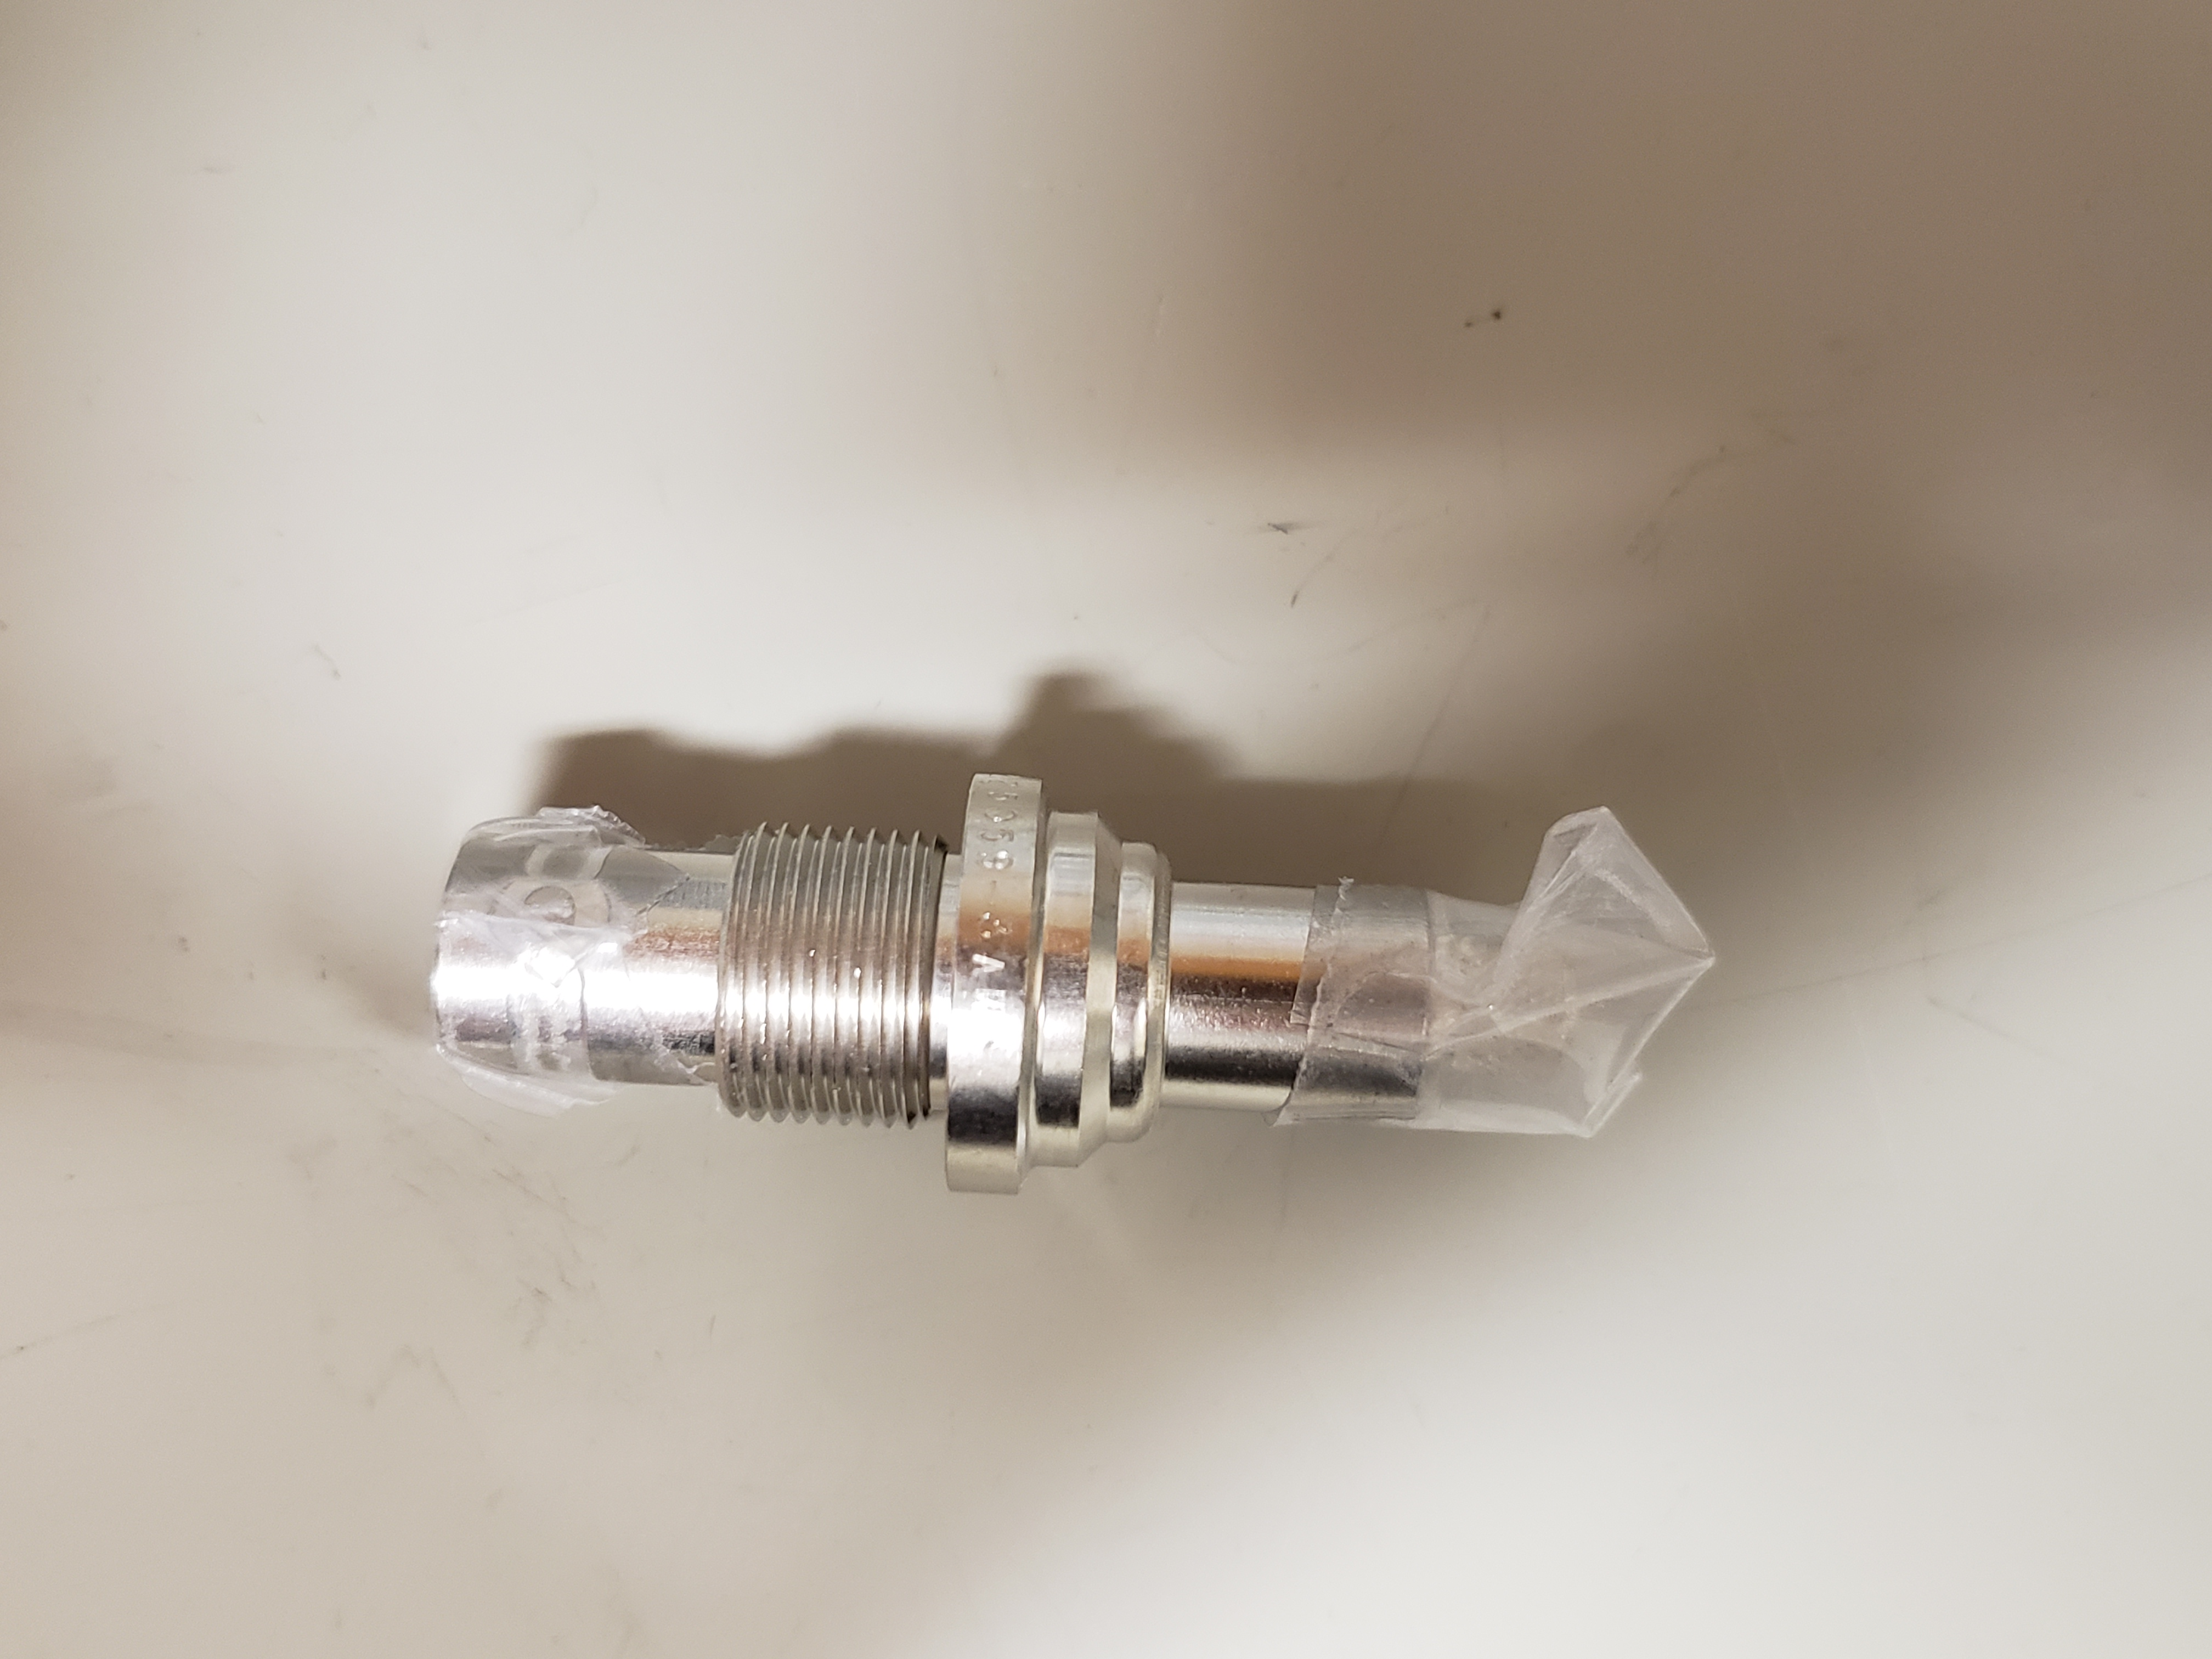
\includegraphics[angle=-90,origin=c,width=2in]{SHVJackBodyTaped}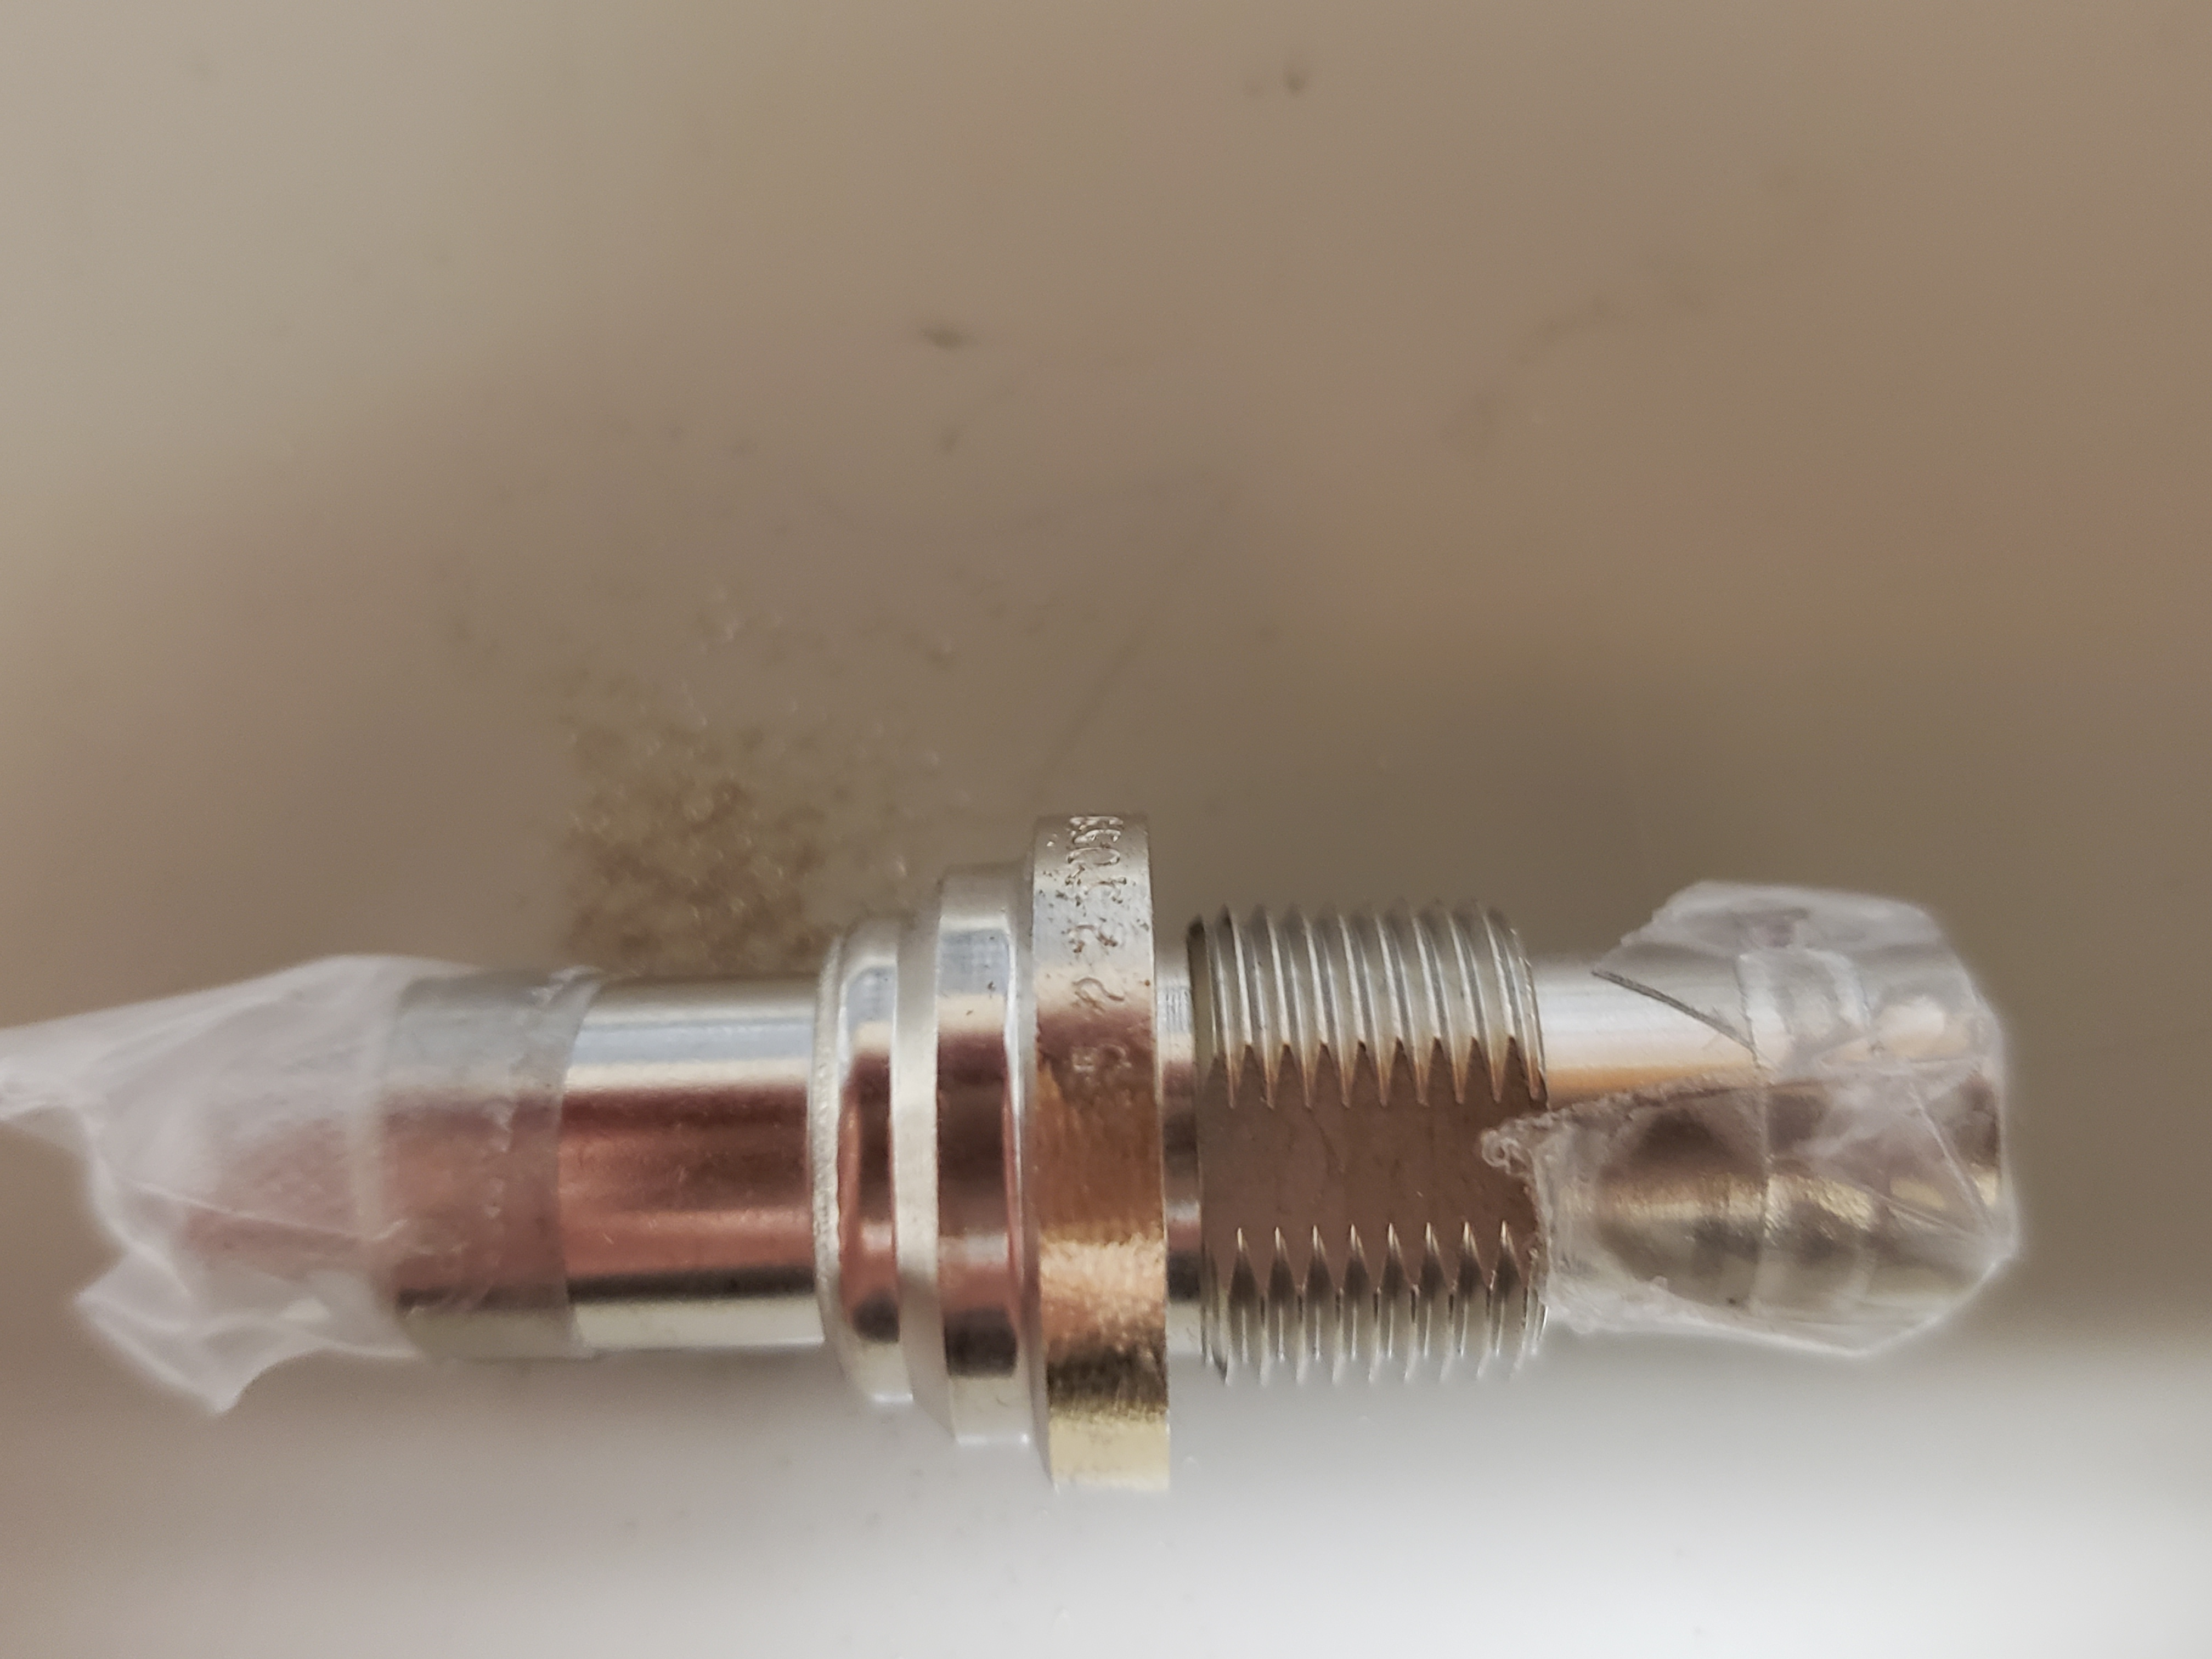
\includegraphics[angle=90,origin=c,width=2in]{SHVJackNickelPartiallyRemoved}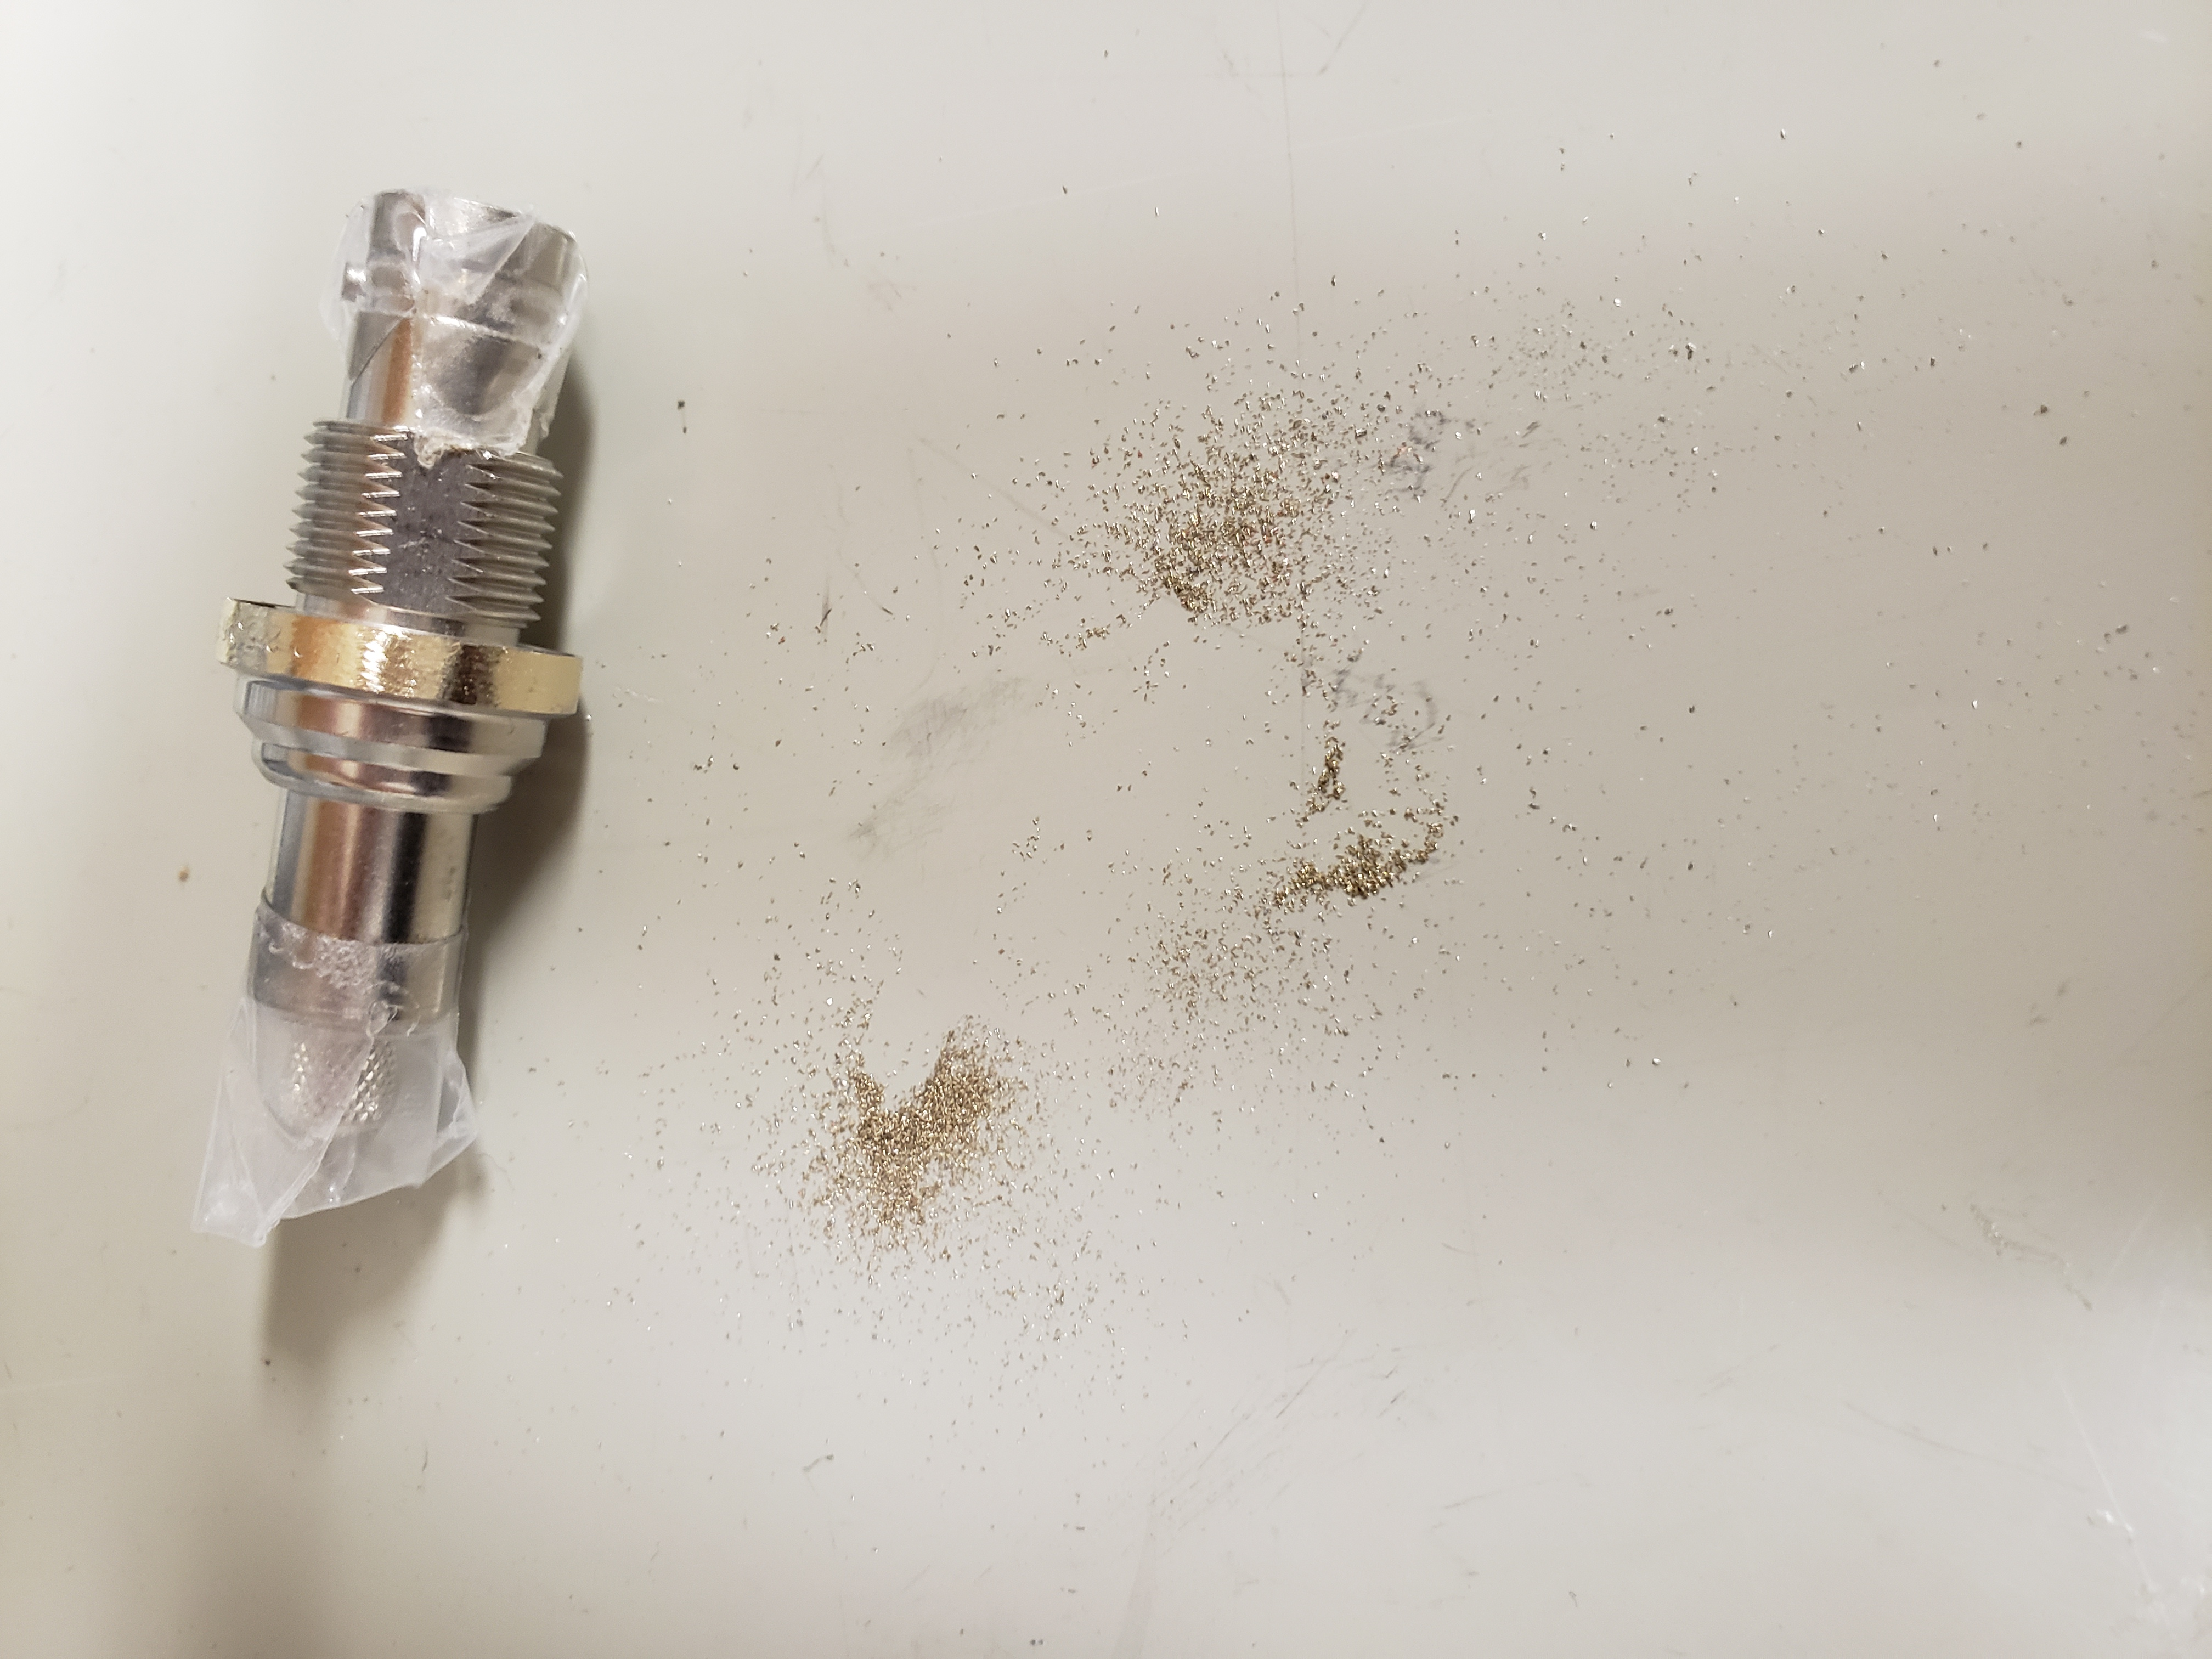
\includegraphics[angle=-90,origin=c,width=2in]{SHVJackNickelRemoved}\caption{\label{fig:SHVjackPlating}Left: SHV jack body with openings taped
over. Center: some of nickel plating filed off revealing underlying
brass. Right: all nickel from surface to be soldered removed, also
showing the dust of all the material that was removed.}

\end{figure}
\item (Optional) Tin the uncoated surface of the SHV jack body to ease making
a good solder connection with the tube later.
\begin{enumerate}
\item Use a tip that will provide good heat transfer and set the soldering
iron to it's highest temperature.
\item The entire SHV jack body will be heated to near the solder melting
temperature, use something that doesn't conduct heat well to manipulate
it, like a bunch of paper towels.

\subsubsection*{See figure \ref{fig:TinningSHVjack} for tinning the SHV jack.}
\begin{enumerate}
\item Apply a small blob of solder to the uncoated surface of the SHV jack
body.
\item Spread the blob of solder around the surface until it covers the entire
surface where the nickel was removed.
\item Remove any excess solder with fluxed solder wick.
\begin{figure}[H]
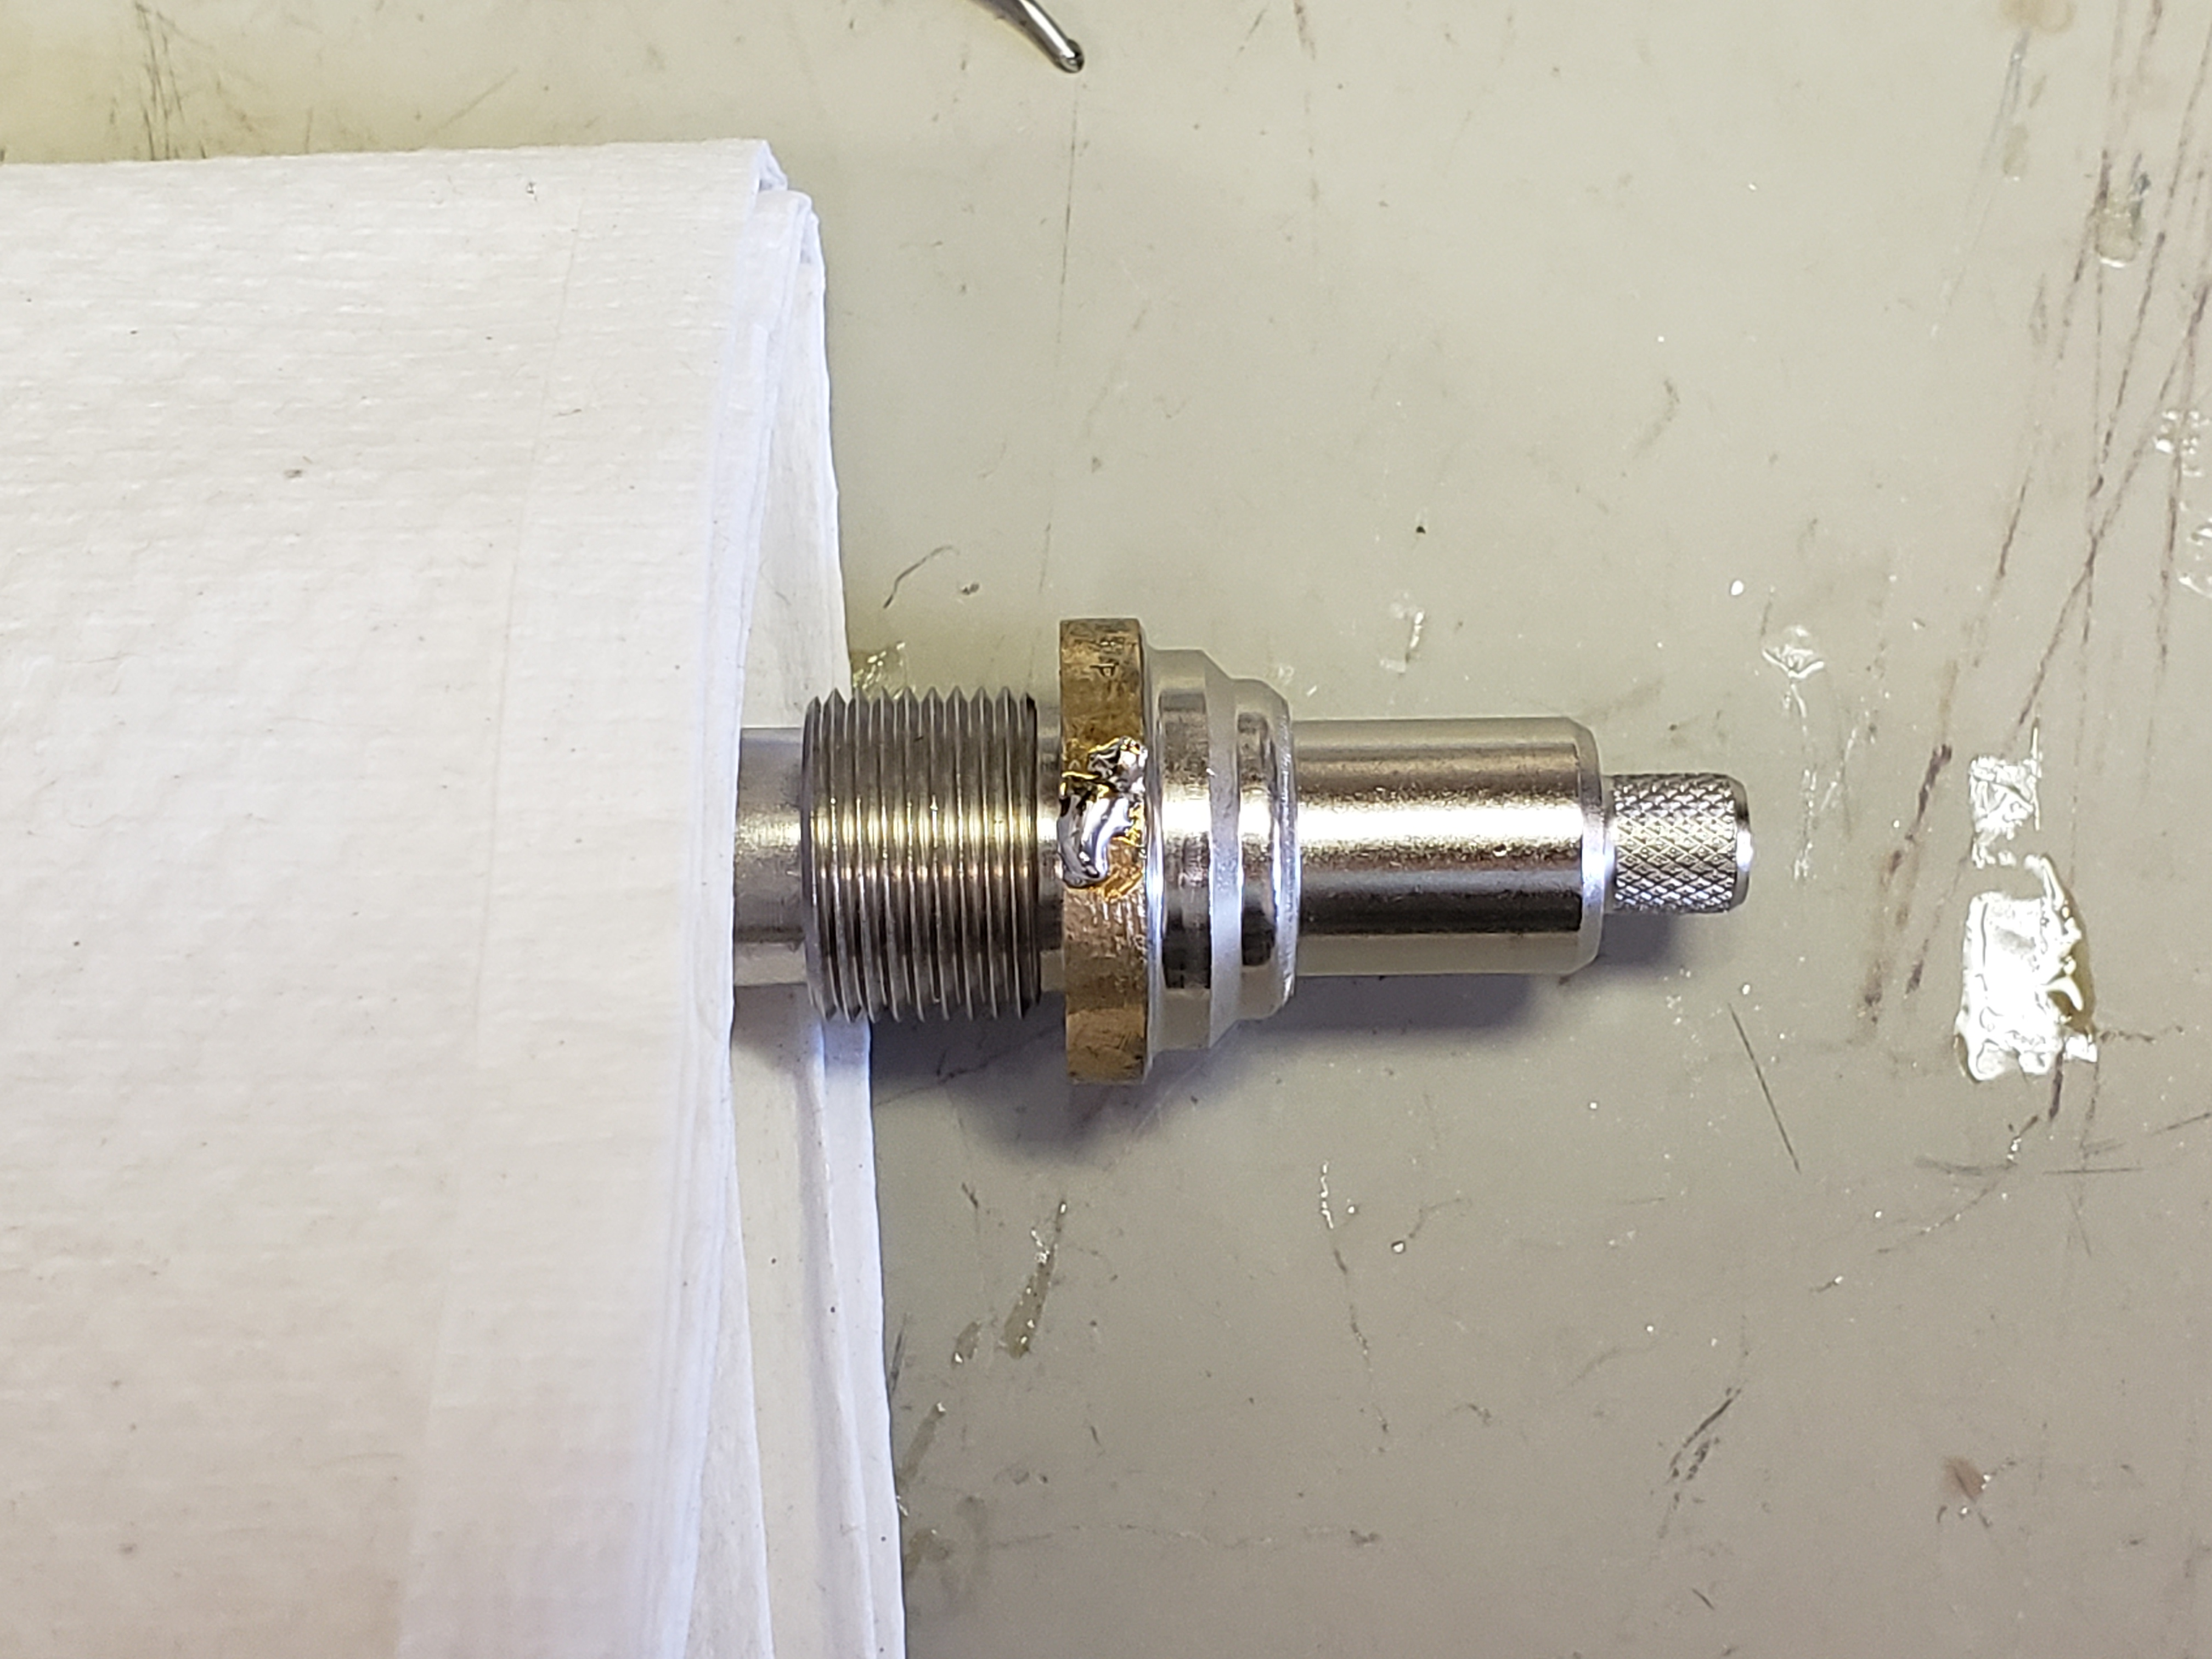
\includegraphics[width=3in]{SHVJackBodyInitialSolderBlob}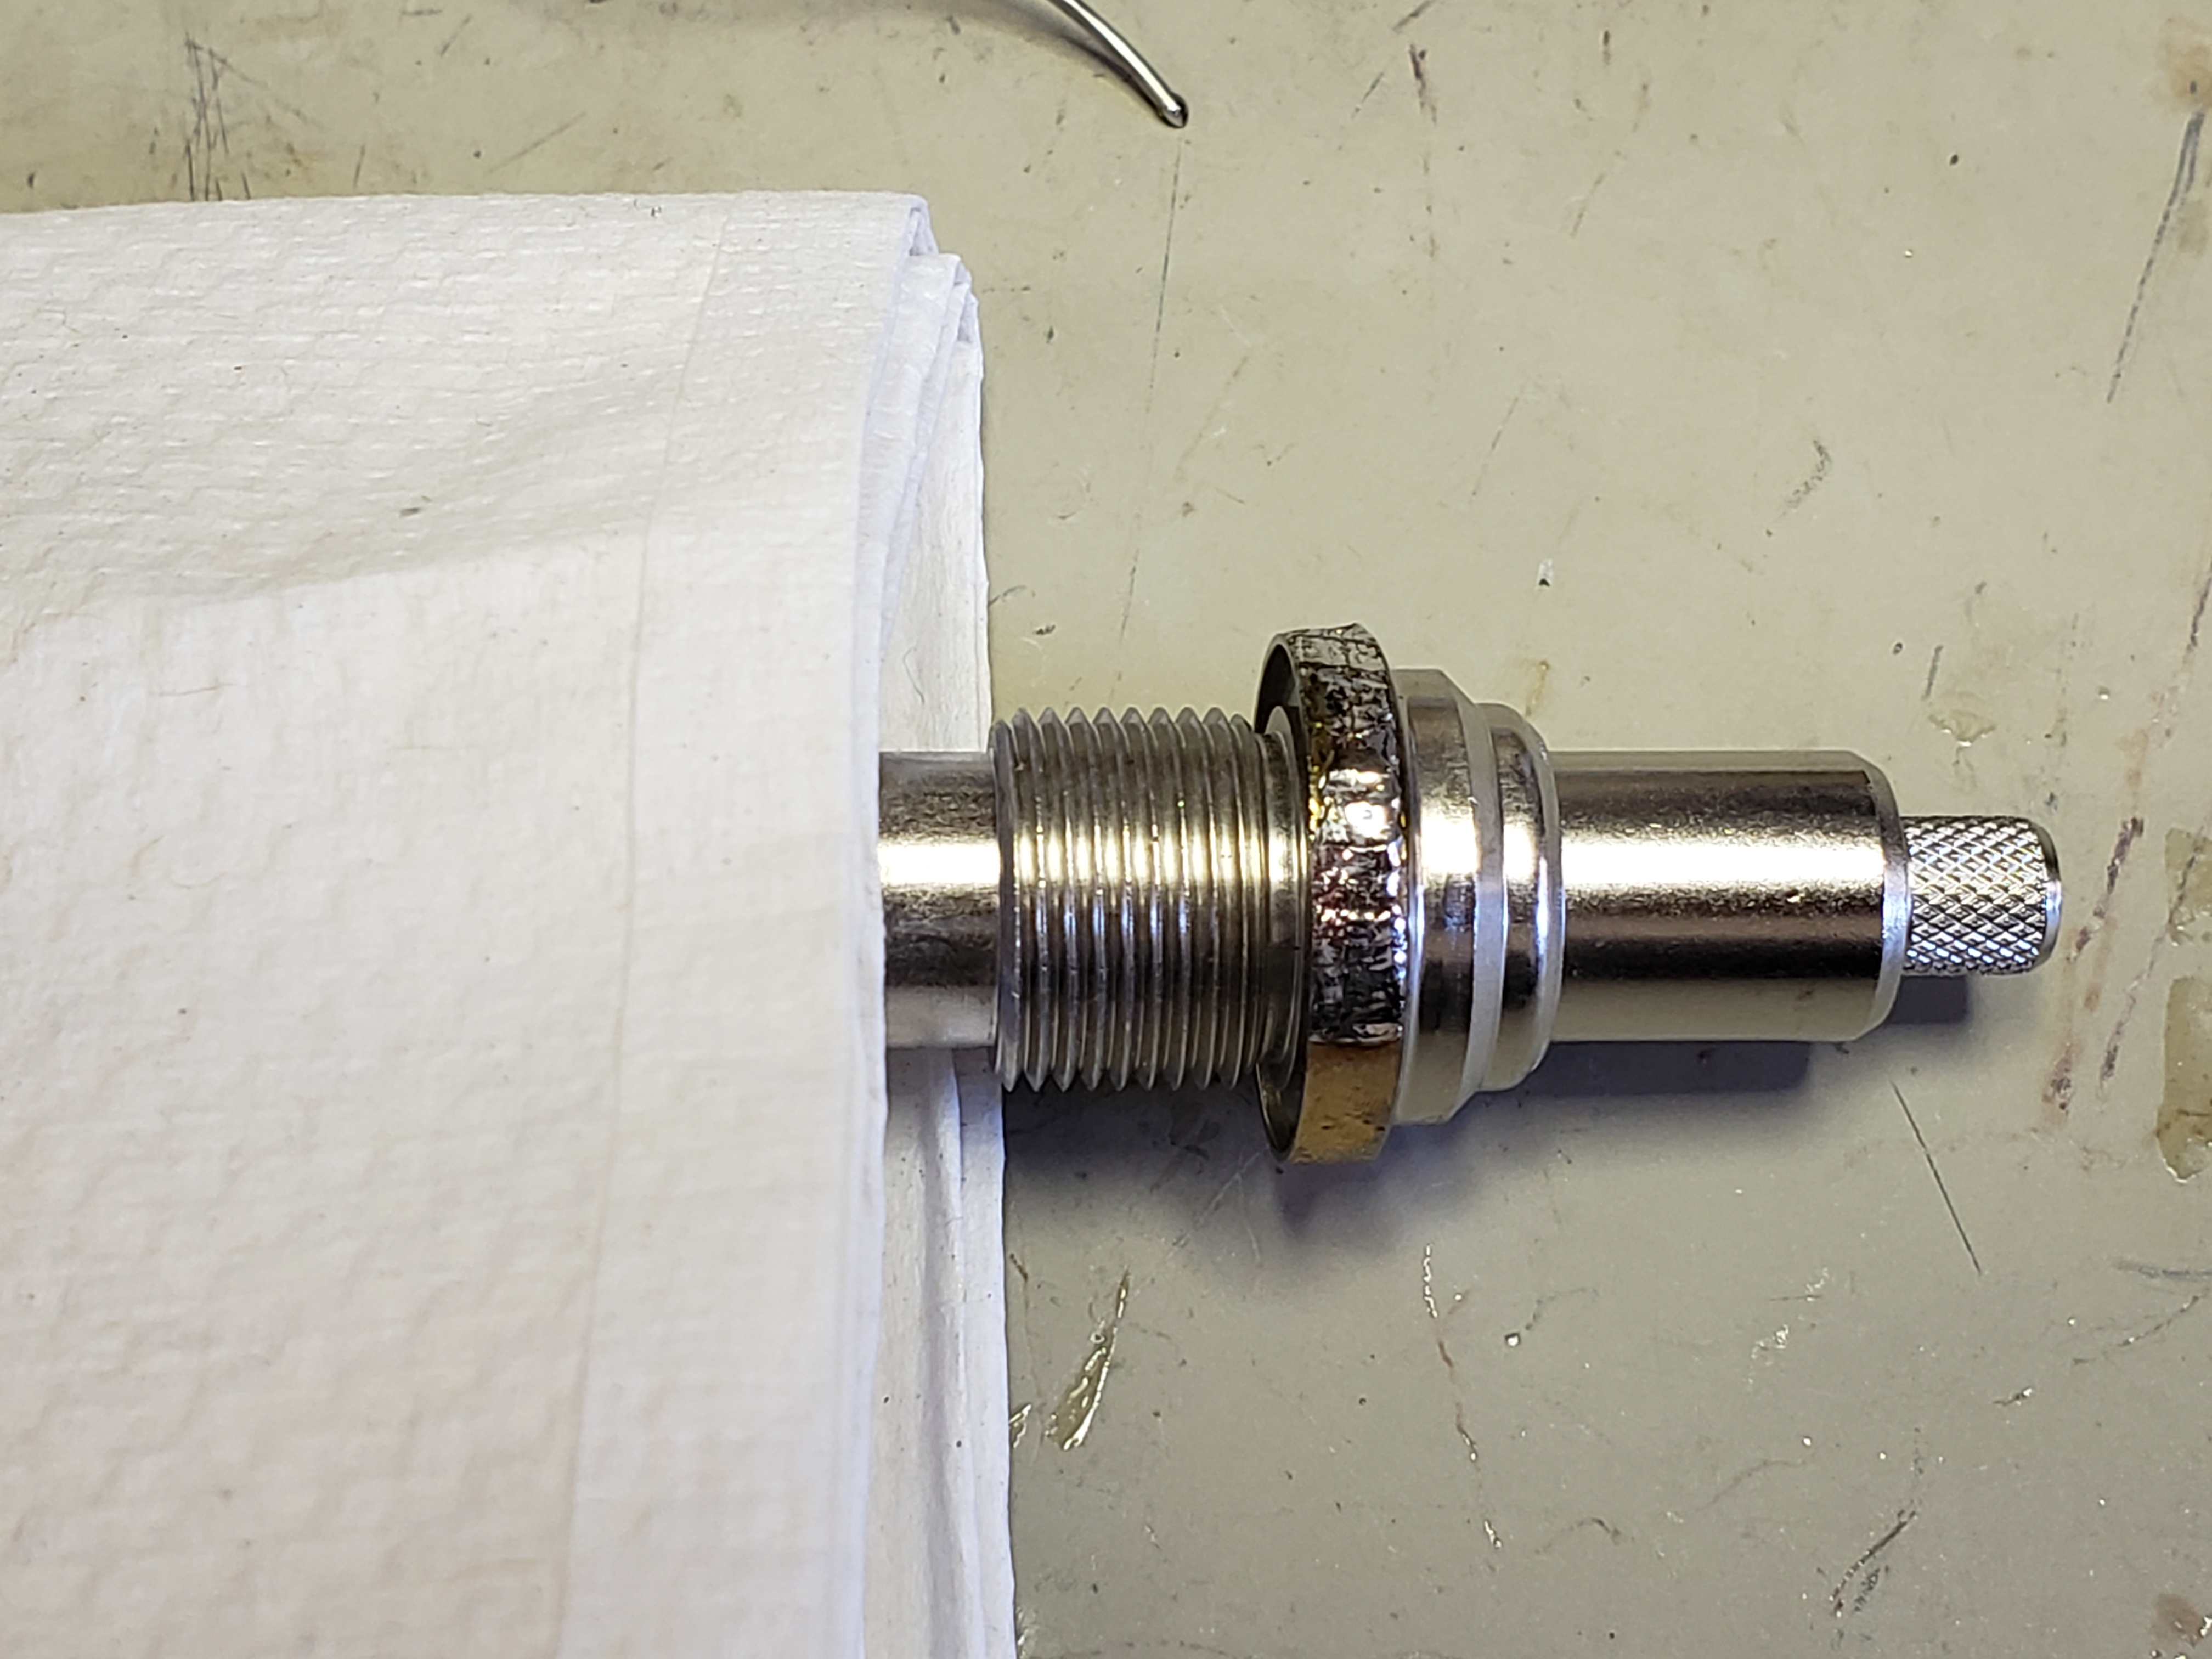
\includegraphics[width=3in]{SHVJackBodySpreadingSolder}

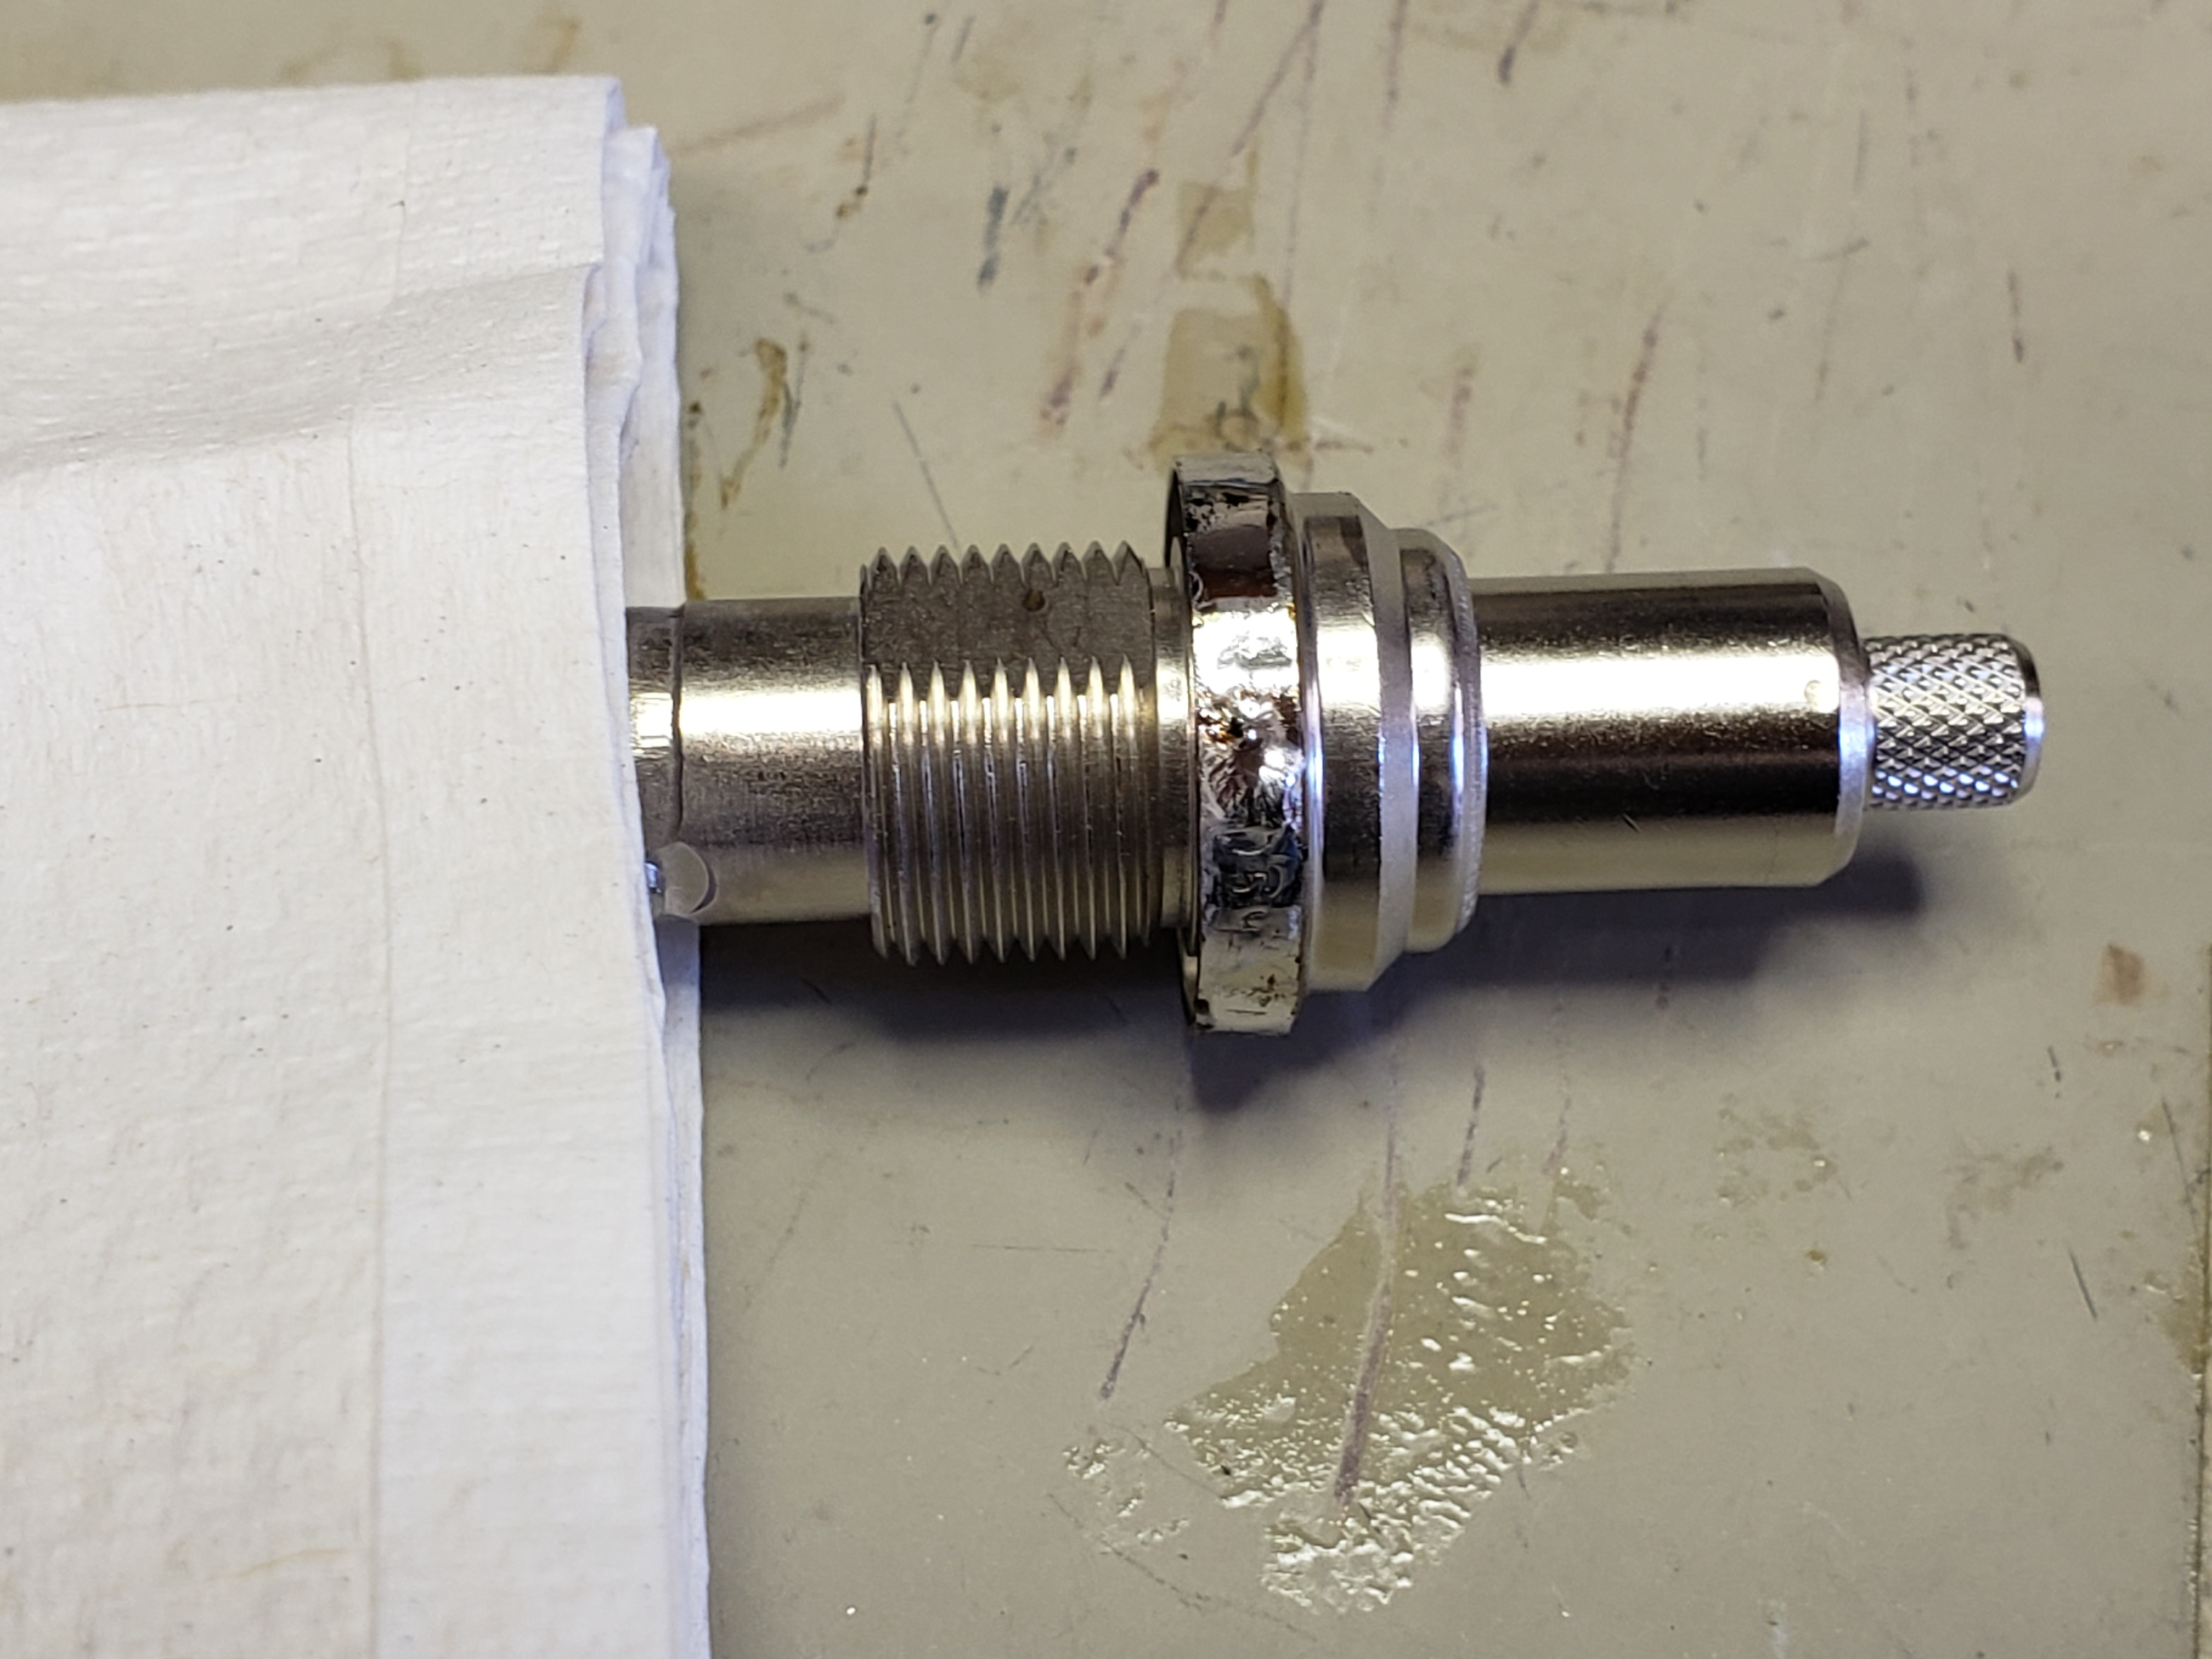
\includegraphics[width=3in]{SHVJackBodyExtraSolder}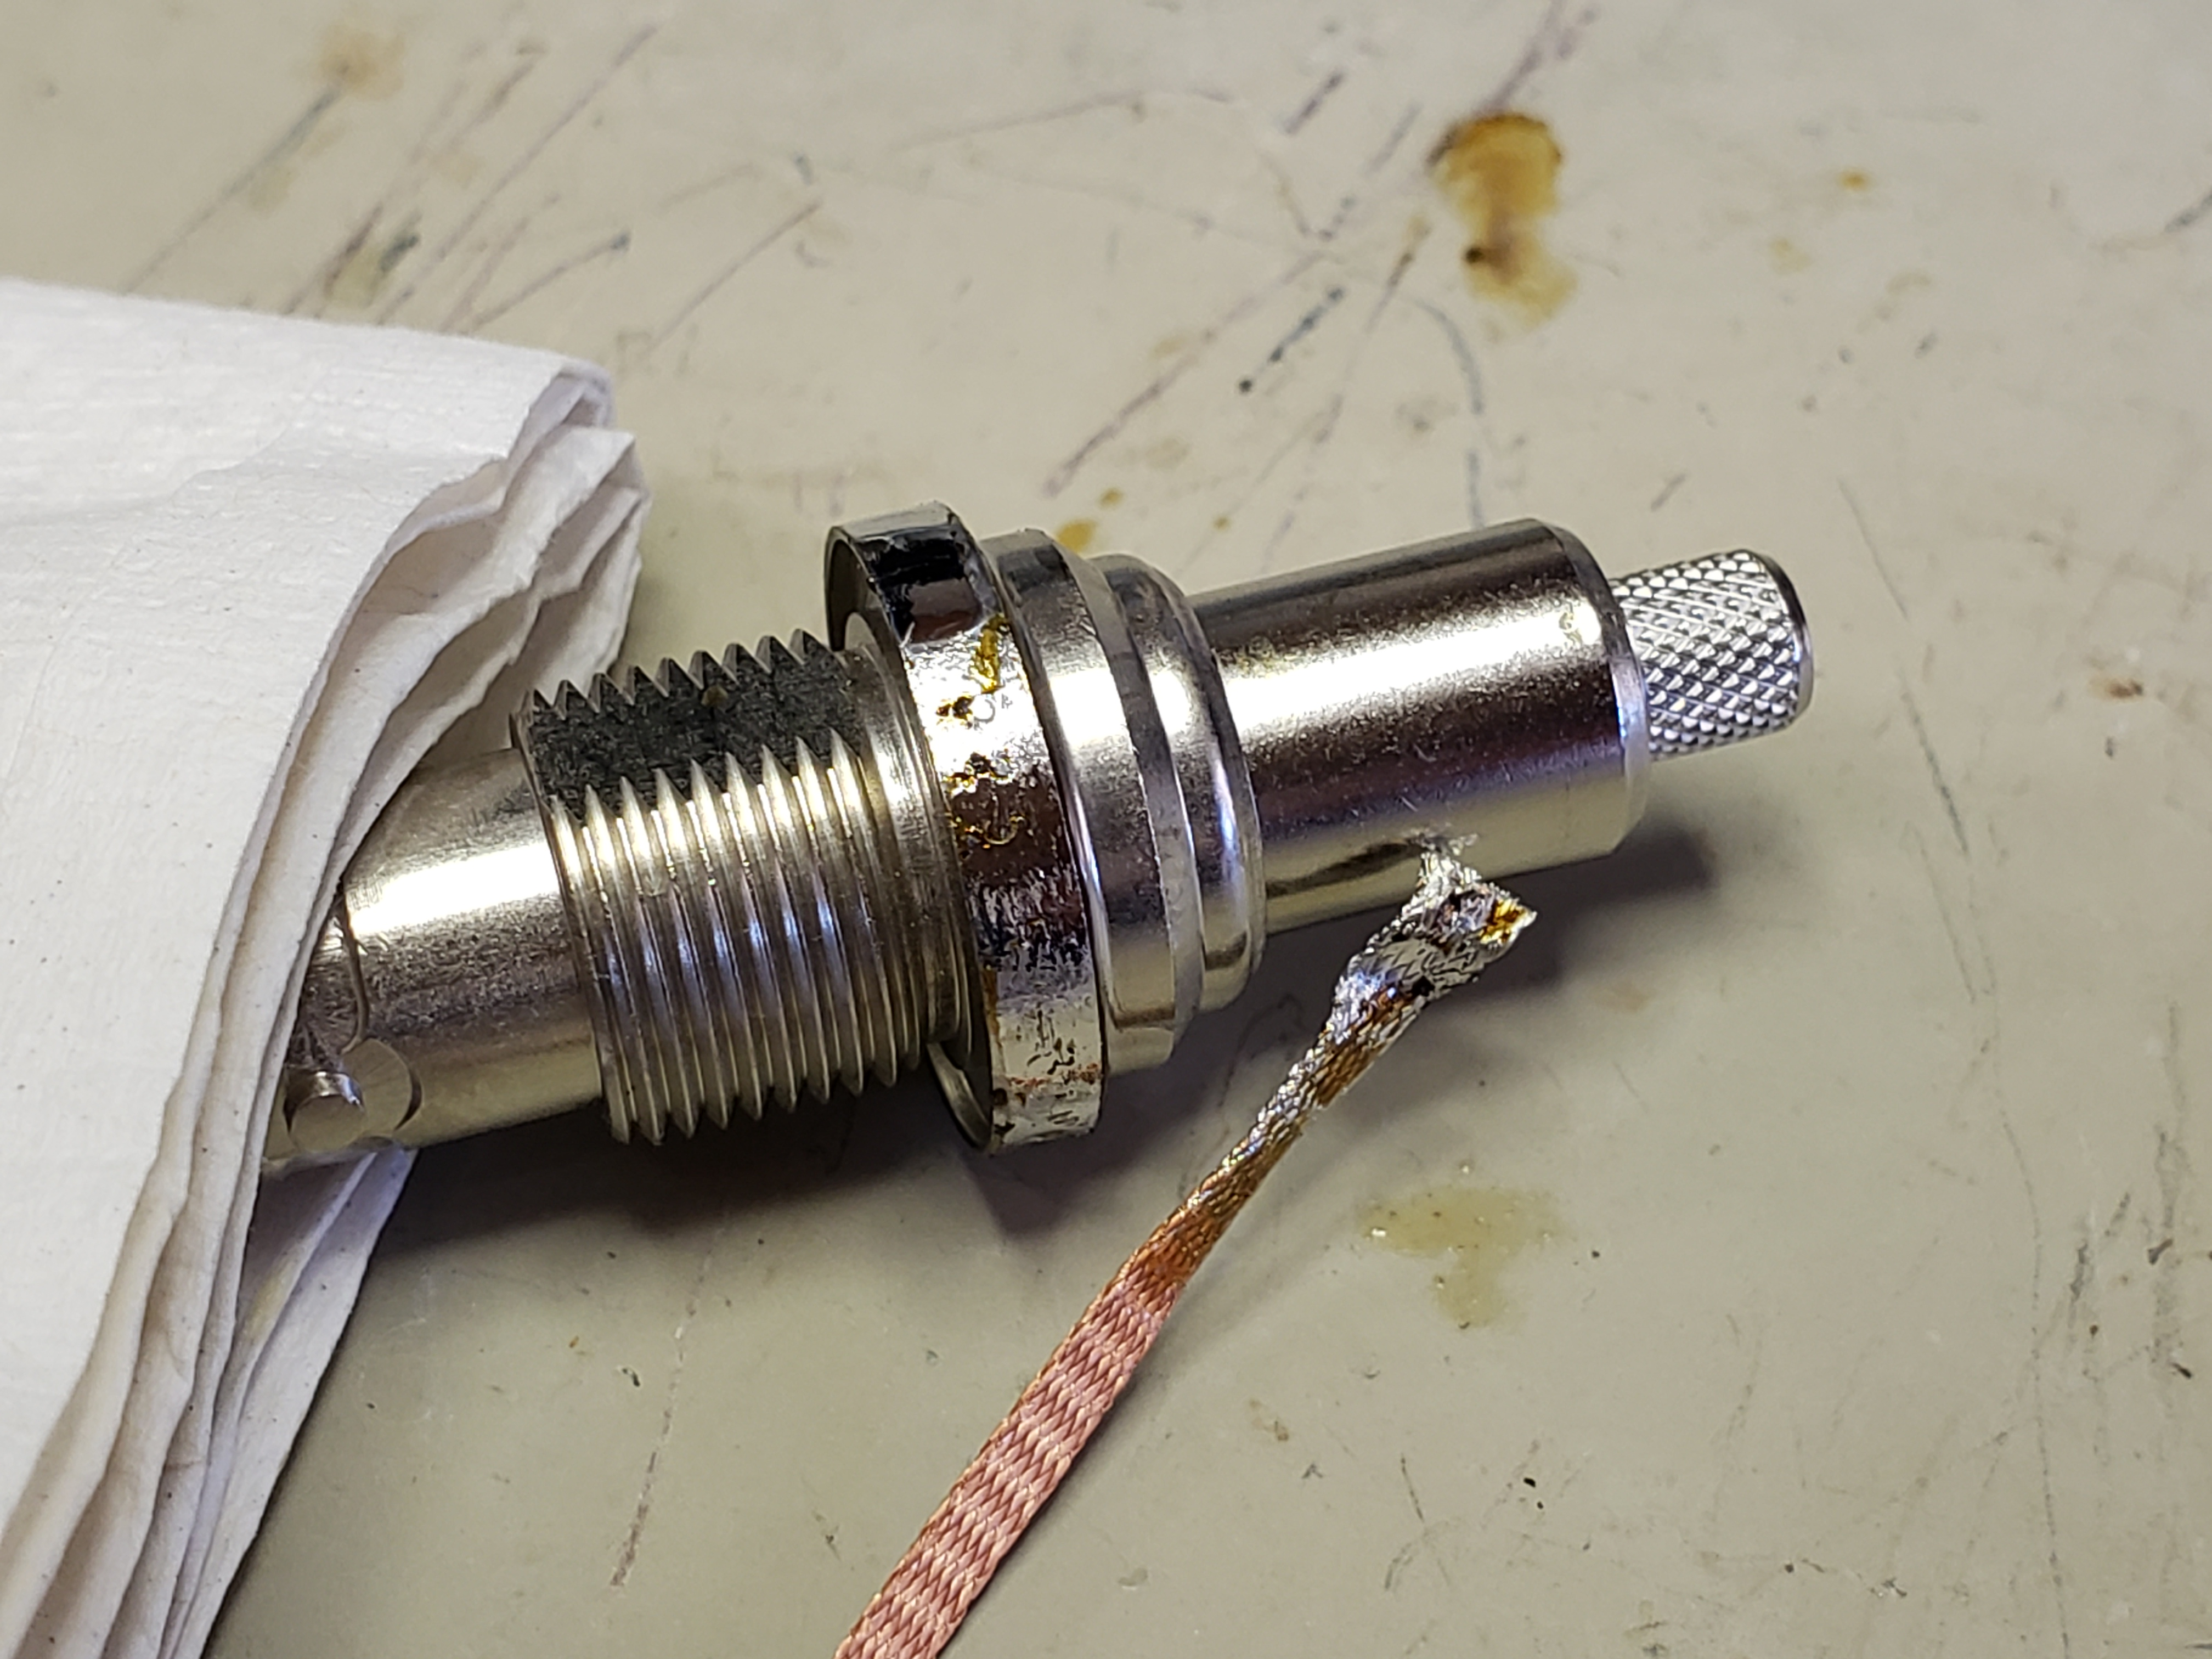
\includegraphics[width=3in]{SHVJackBodyExtraSolderRemoved}\caption{\label{fig:TinningSHVjack}Top left: a small blob of solder applied
to edge of SHV jack body. Top right: spreading the solder around the
edge. Bottom left: extra solder after covering entire edge. Bottom
right: SHV jack body after excess solder wicked away.}
\end{figure}
\end{enumerate}
\end{enumerate}
\end{enumerate}

\subsection{Install SHV pin on resistor}
\begin{enumerate}
\item Check that the resistor end which will have the pin fits freely in
the connector, for the Ohmite MOX1125231006FE resistors most easily
fit in the connect, but one was found that wouldn't fit without being
sanded down. It needs to have enough of a gap that oil can easily
flow in. If one end doesn't fit try the other end or a different resistor
(some resistors are a little thicker than others) and use the wide
resistor for the output of the filter. If no resistors fit the bulge
can be sanded down to be even with the rest of the resistor.
\item Cut the fit tested lead of the resistor down to the central conductor
length in the connector trim recommendations, 6 mm for TE Connectivity
AMP Connectors 5225059-3.
\item Solder the pin on the lead.

\subsubsection*{See figure for \ref{fig:PinSoldering} soldering the pin on the resistor.}
\begin{enumerate}
\item Tin the lead, there should be enough solder that will fill the gap
in the pin but not so much it comes out of the pin once assembled.
If there's a solder bulge on the lead large enough that it can't be
pushed into the pin then it's enough to ensure contact with the pin
once reheated and inserted.
\item Heat the pin with the lead held against the opening of the pin until
the solder melts and the lead slides into the pin, no solder should
flow out the escape hole in the pin.
\item Let the solder cool then ensure there is a good connection by gently
pulling on the pin and resistor to be sure they doesn't come apart.
\begin{figure}[H]
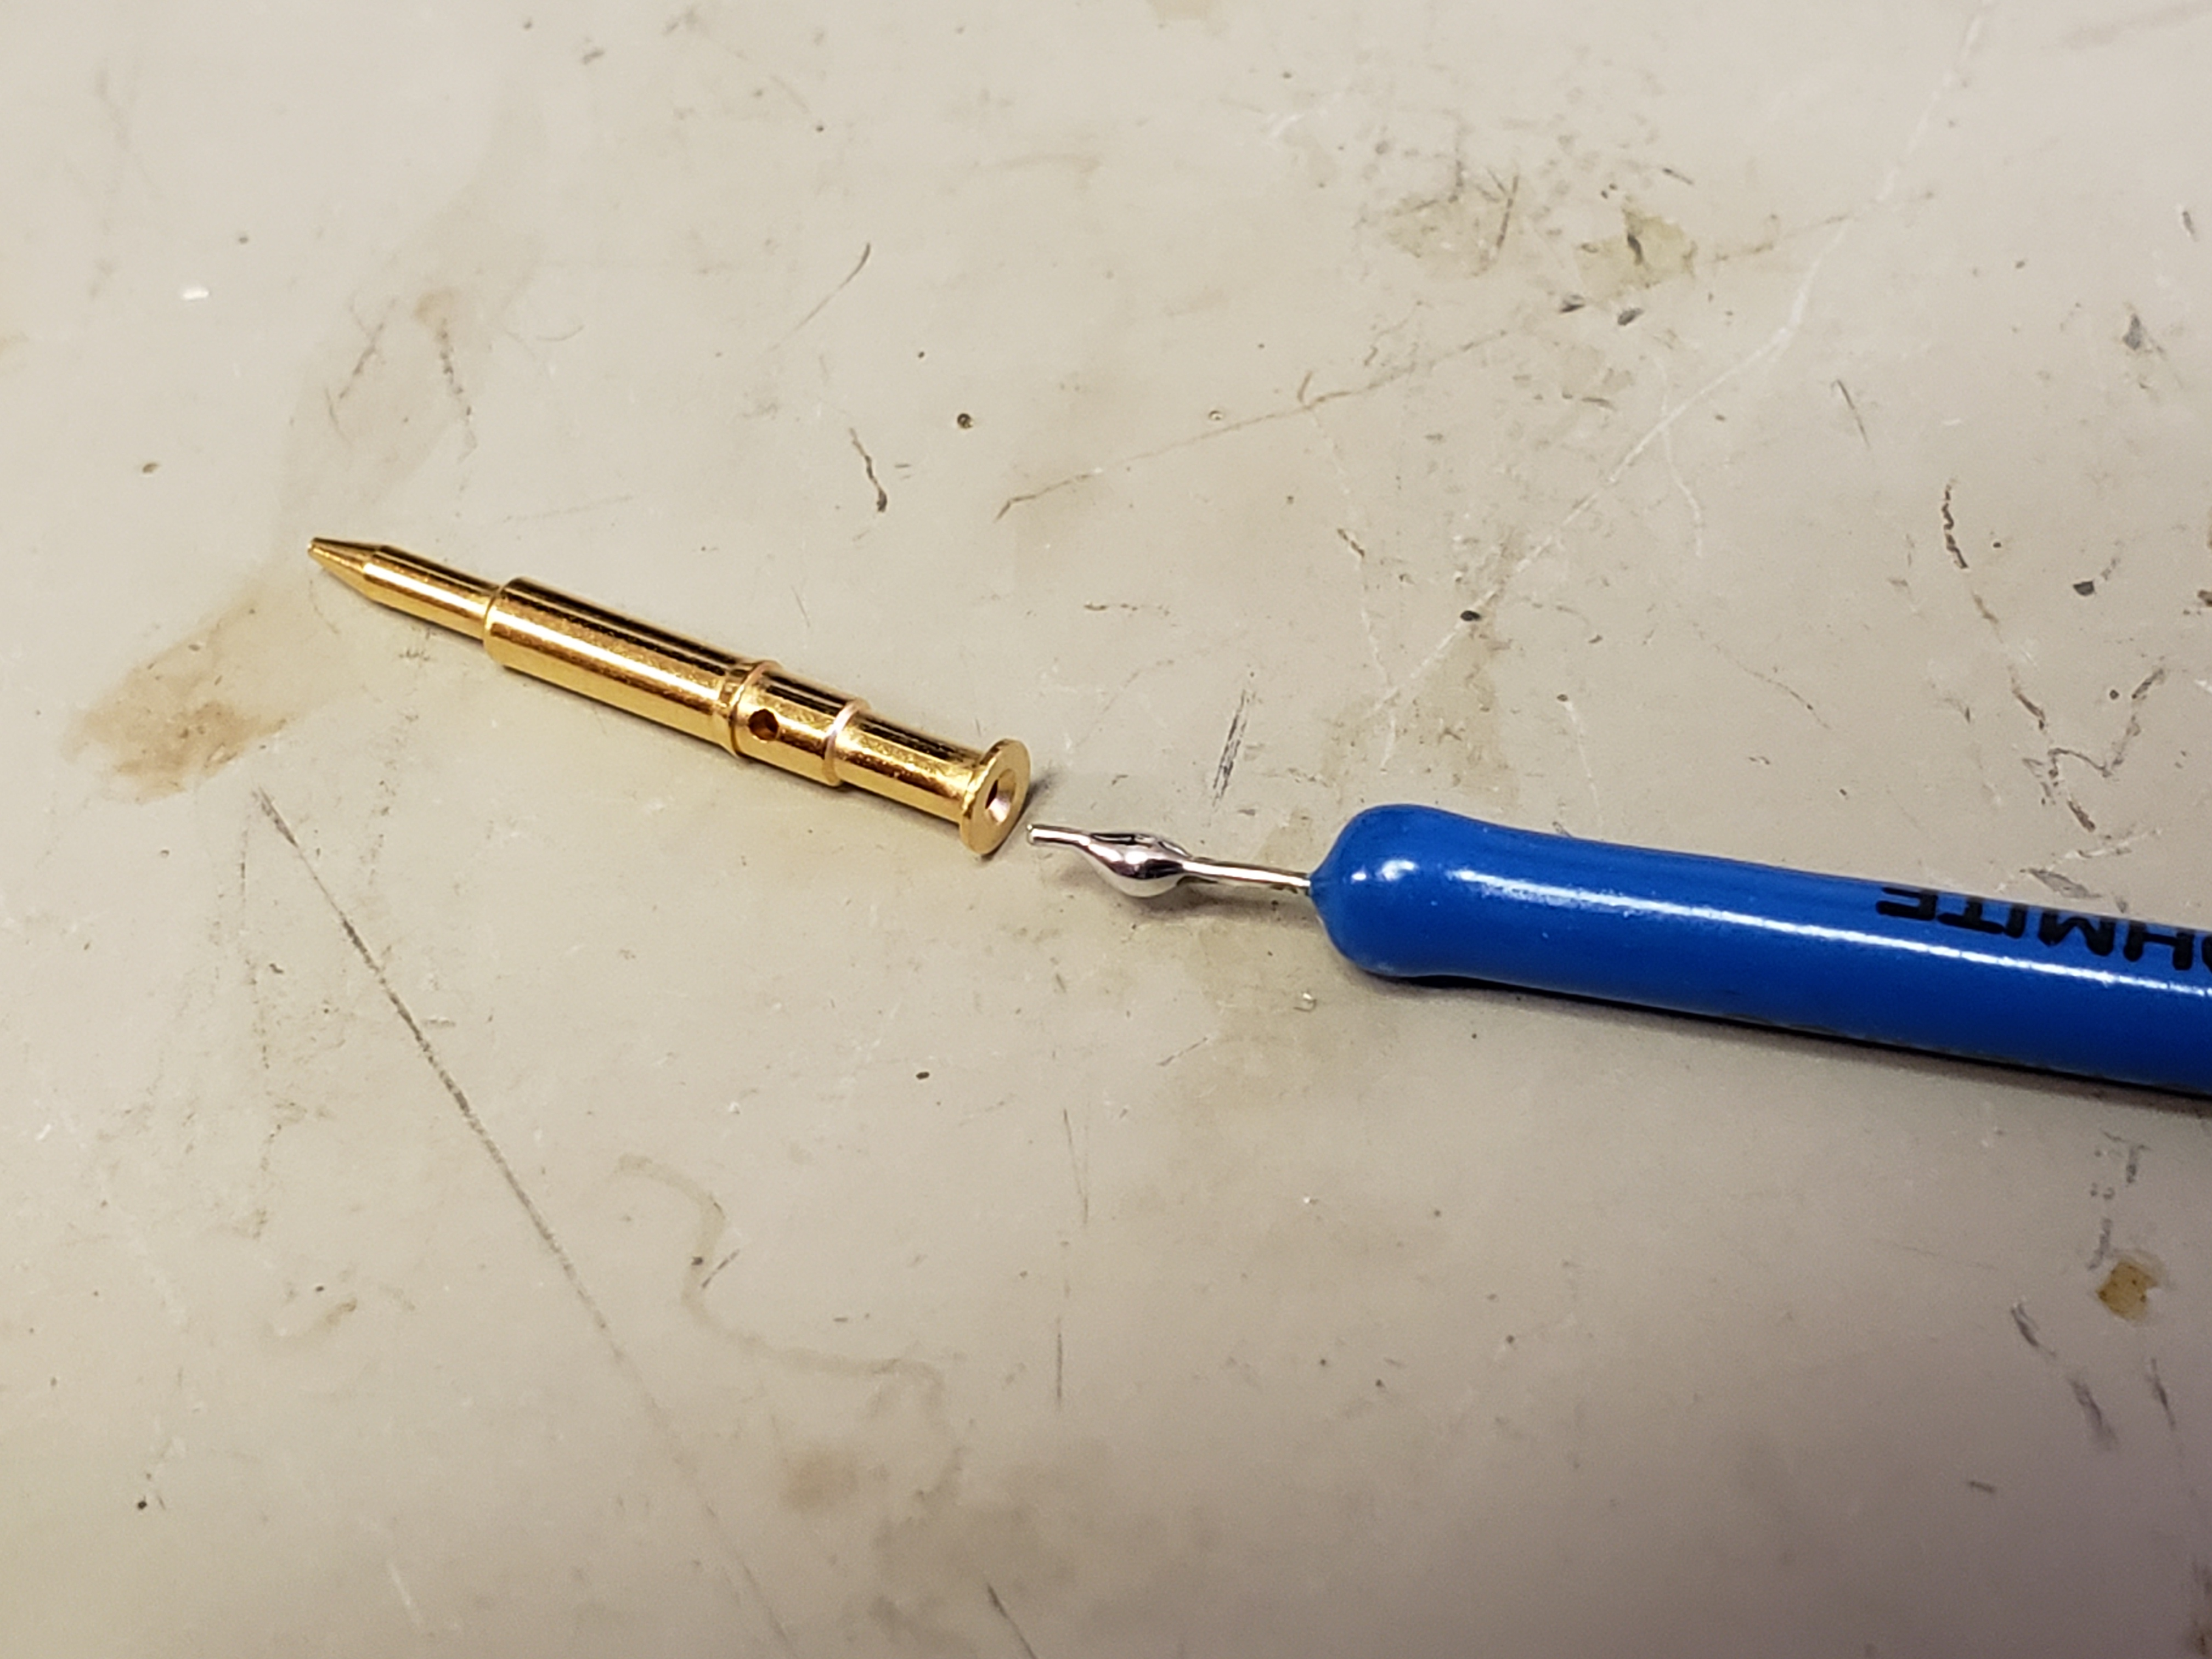
\includegraphics[width=2in]{SHVPinResistorSolderBlob}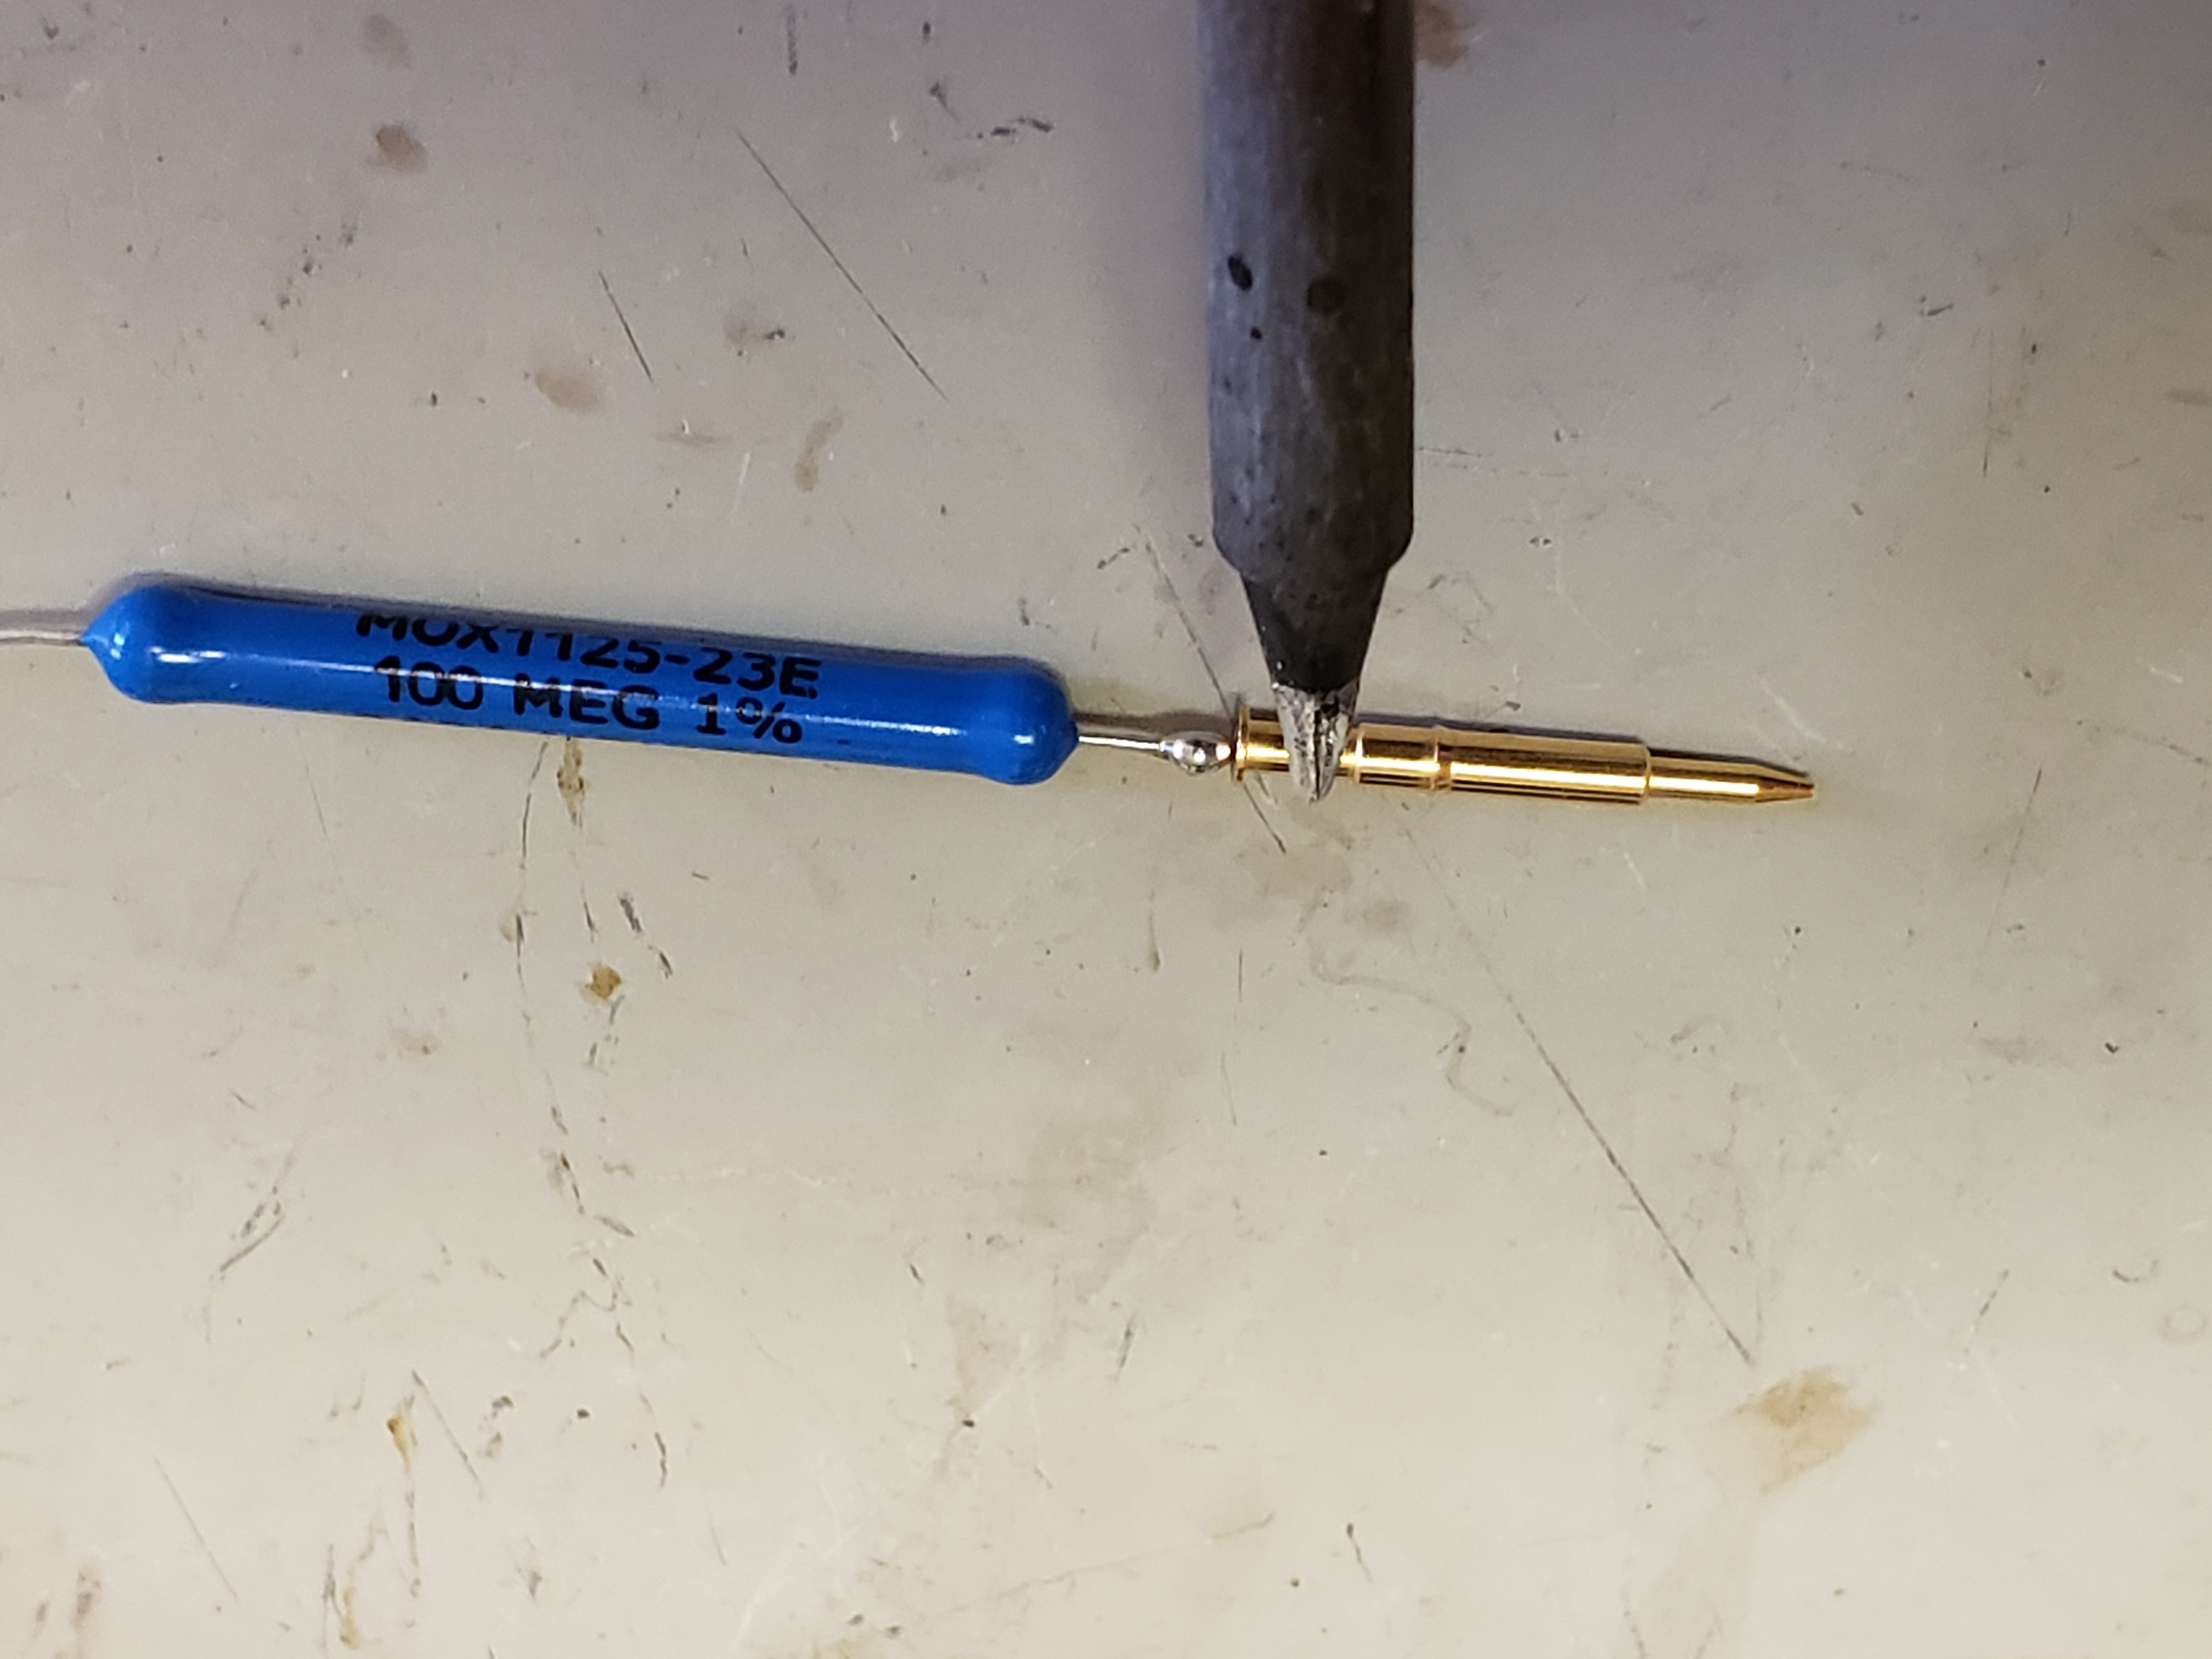
\includegraphics[width=2in]{SHVPinInsertingResistor}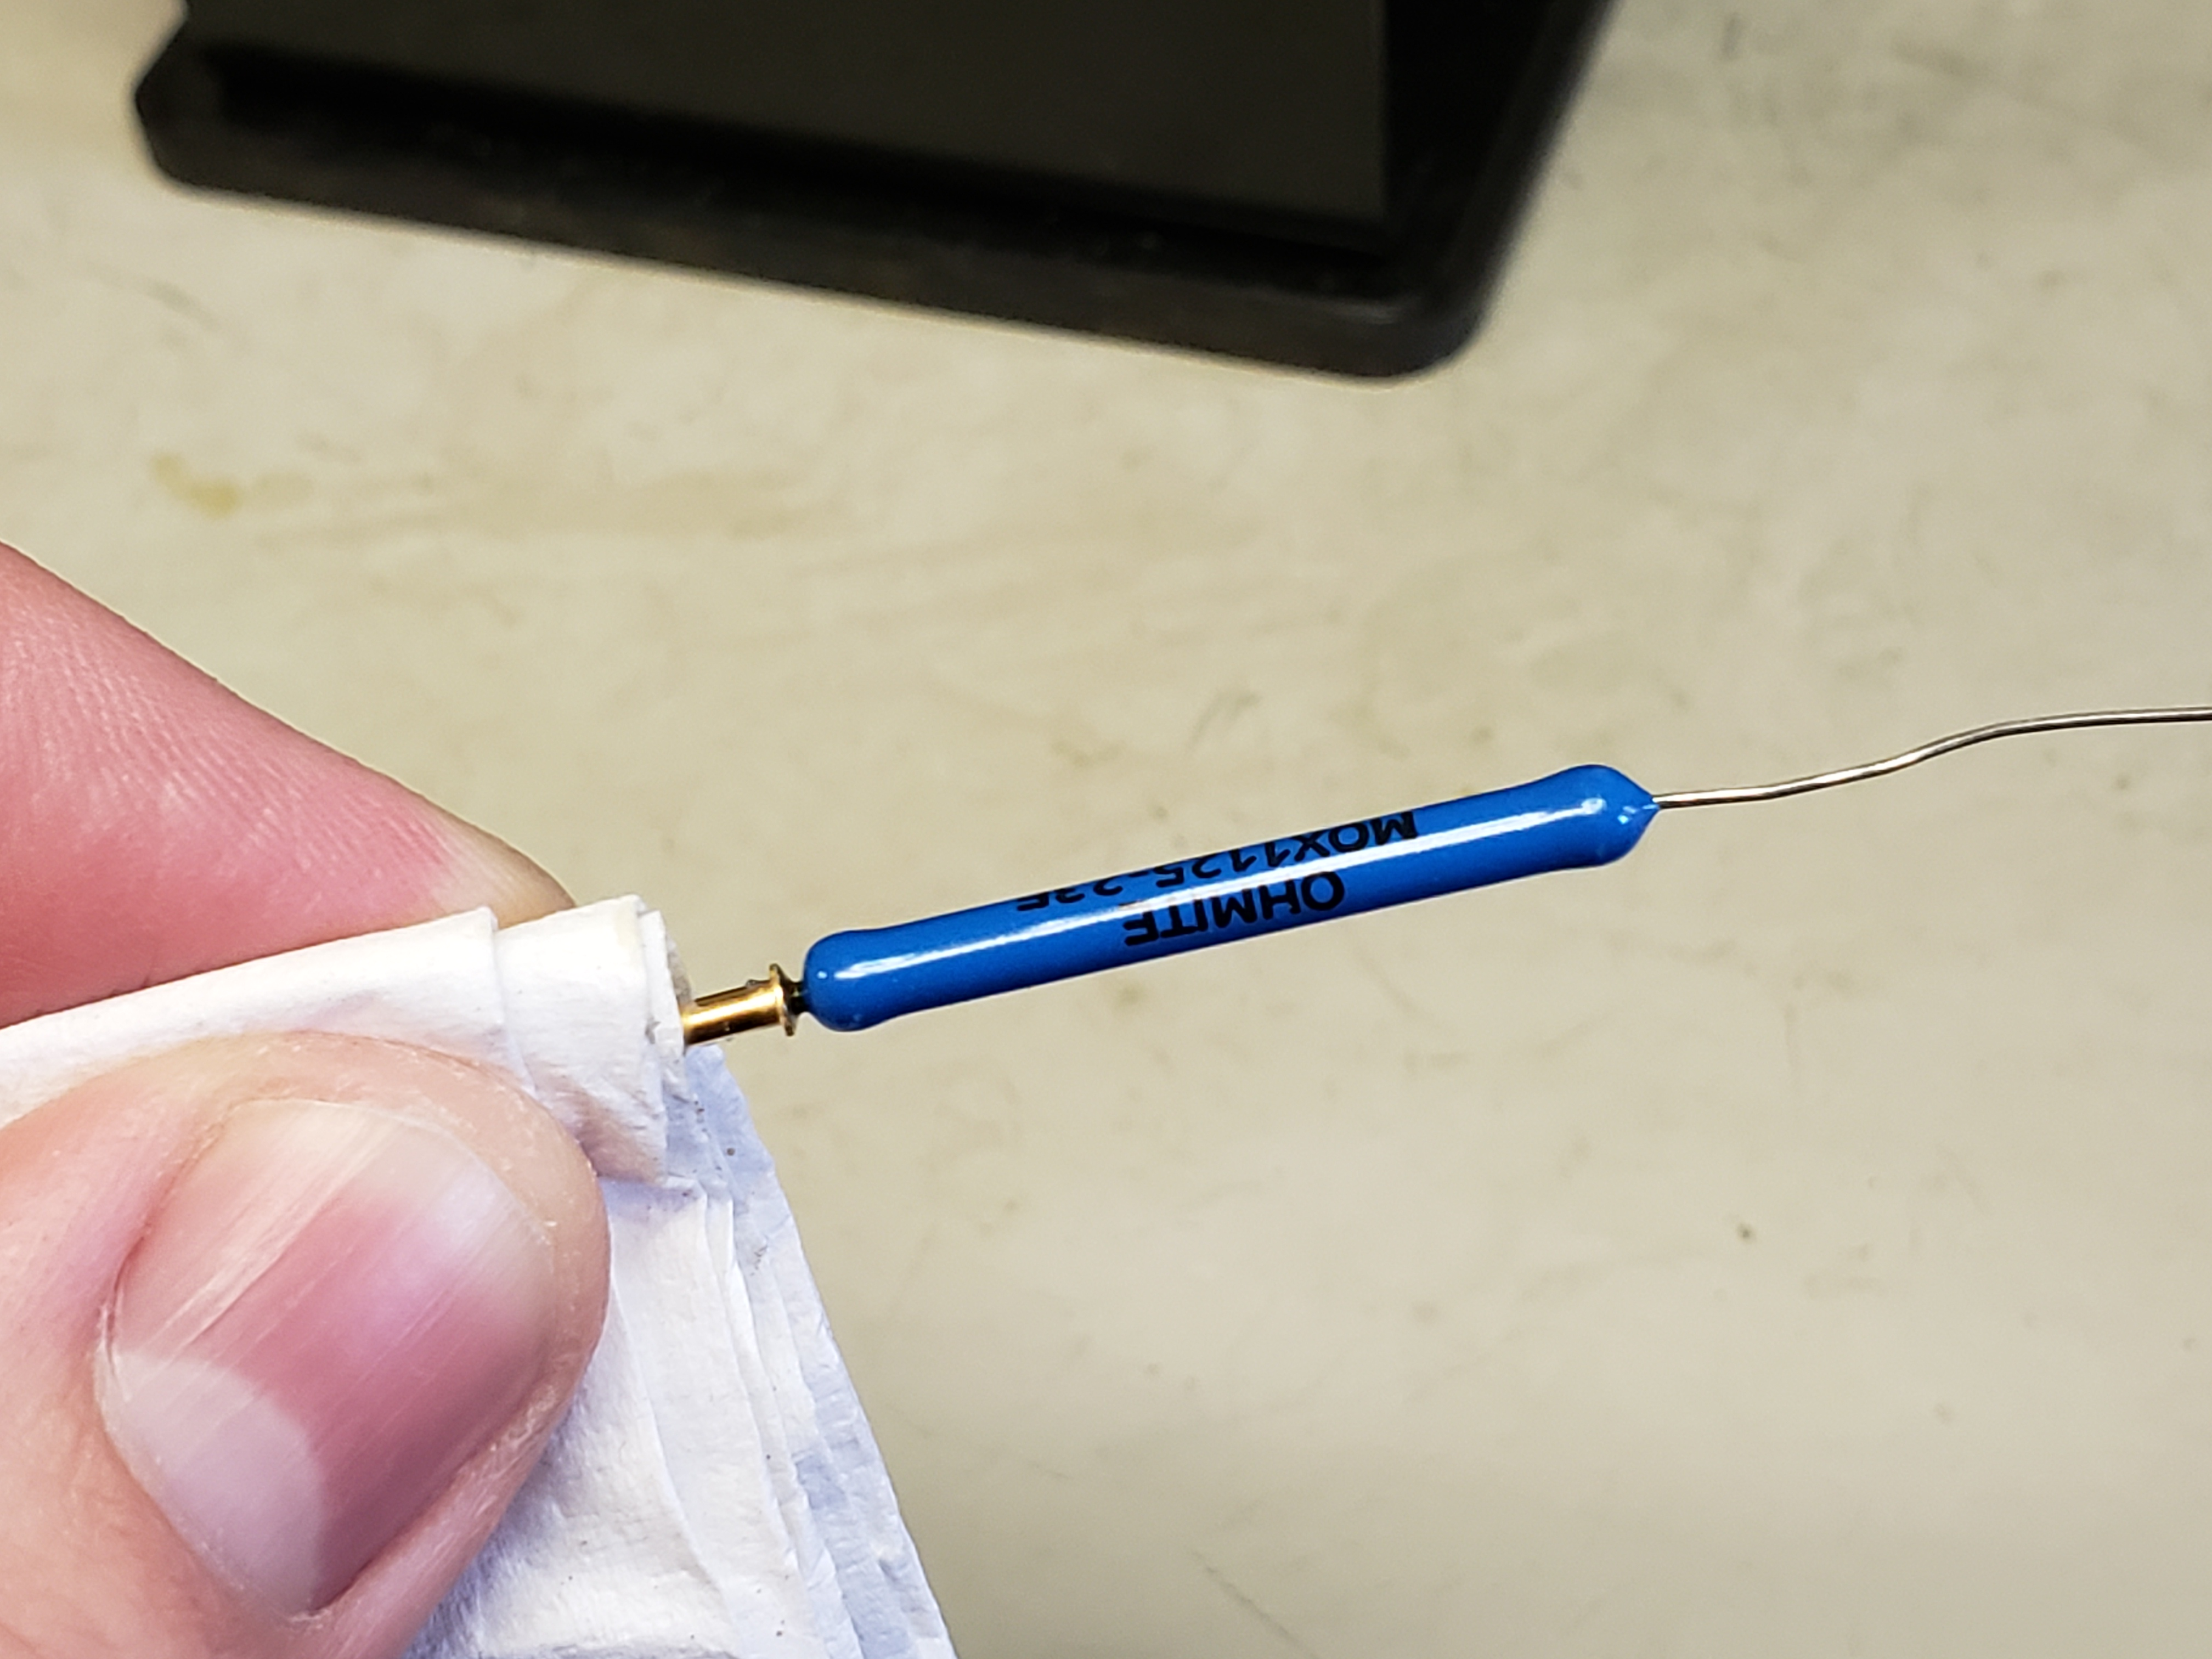
\includegraphics[width=2in]{SHVPinWithResistor}

\caption{\label{fig:PinSoldering}Left: solder blob on resistor lead ready
for insertion into SHV pin. Center: inserting resistor by heating
SHV pin. Right: Assembled SHV pin and resistor held with paper towels
because the pin is still hot.}
\end{figure}
\end{enumerate}
\end{enumerate}

\subsection{Install resistor and SHV pin in SHV jack.}
\begin{enumerate}
\item Assemble the parts in a clean room or wear gloves at a minimum. Any
residual oil from hands can lead to excessive leakage currents on
high voltage components. 
\item Clean the SHV jack and the resistor with the SHV pin well with isopropyl
alcohol.
\item Prepare for epoxy application. If a centrifuge and/or vacuum chamber
will be used make sure they are ready to go so the epoxy can be rapidly
degassed and applied while it still flows easily. Read the rest of
the instructions in this section ahead of time.

\subsubsection*{It is recommend to degassing the epoxy in a centrifuge to remove
any bubbles that formed during mixing that could cause partial discharges.}
\begin{enumerate}
\item Fill a small syringe with the mixed epoxy, cap it, and place it dispenser
side down in a disposable test tube. The tube is keep the centrifuge
clean in the likely event some epoxy spills.
\item Balance the centrifuge with an identical test tube and syringe filled
with the same weight of water.
\item Run the centrifuge at 1000 rpm for 3 minutes, too high and it will
separate back out.
\item Keep the syringe pointed down so the air bubble stays at the plunger
until ready for application.
\end{enumerate}
\item Hold the SHV pin and resistor pin side up so any epoxy that flows
during application will coat the resistor and not the pin. Apply a
small amount of epoxy to the region where the pin meets the resistor.
It only needs to be enough to keep oil from leaking through the pin
hole, it is not necessary to pot the connector with epoxy. Don't get
any epoxy past the chamfered ridge a little further from the pin tip
than center, that's the mating surface for the SHV connector.
\item Fully insert the pin into the SHV jack then invert the SHV jack and
set it pin side down while the epoxy cures, so the epoxy can flow
around the pin and form a good seal.

\subsubsection*{It is recommended to vacuum degas the epoxy to drive out any small
bubbles that could cause partial discharges. Only do this if it can
be accomplished within a fraction of the working time of the epoxy.}
\begin{enumerate}
\item Place the SHV jack pin side down in a clear vacuum chamber.
\item Place the remaining epoxy in a small dish inside the same vacuum chamber.
If the vacuum is too low it will boil the epoxy and cause bubbles
instead of remove them.
\item Draw a vacuum of 29 in Hg, if the epoxy in the dish is boiling reduce
vacuum. Wait 2 minutes.
\item Slowly vent the vacuum chamber, this is to collapse any bubbles that
rose to the surface. Agitating the chamber can also help burst bubbles.
\item Repeat this cycle of drawing a vacuum then venting until there are
no bubbles forming in the epoxy in the dish. Then leave the epoxy
to cure under atmospheric pressure. If possible, cure under a pressure
of 60 psig to compressed any remaining bubbles.
\end{enumerate}
\item (Optional) Tape over the gap between the resistor and SHV jack body
to keep dirt out until final assembly.
\end{enumerate}
\begin{figure}
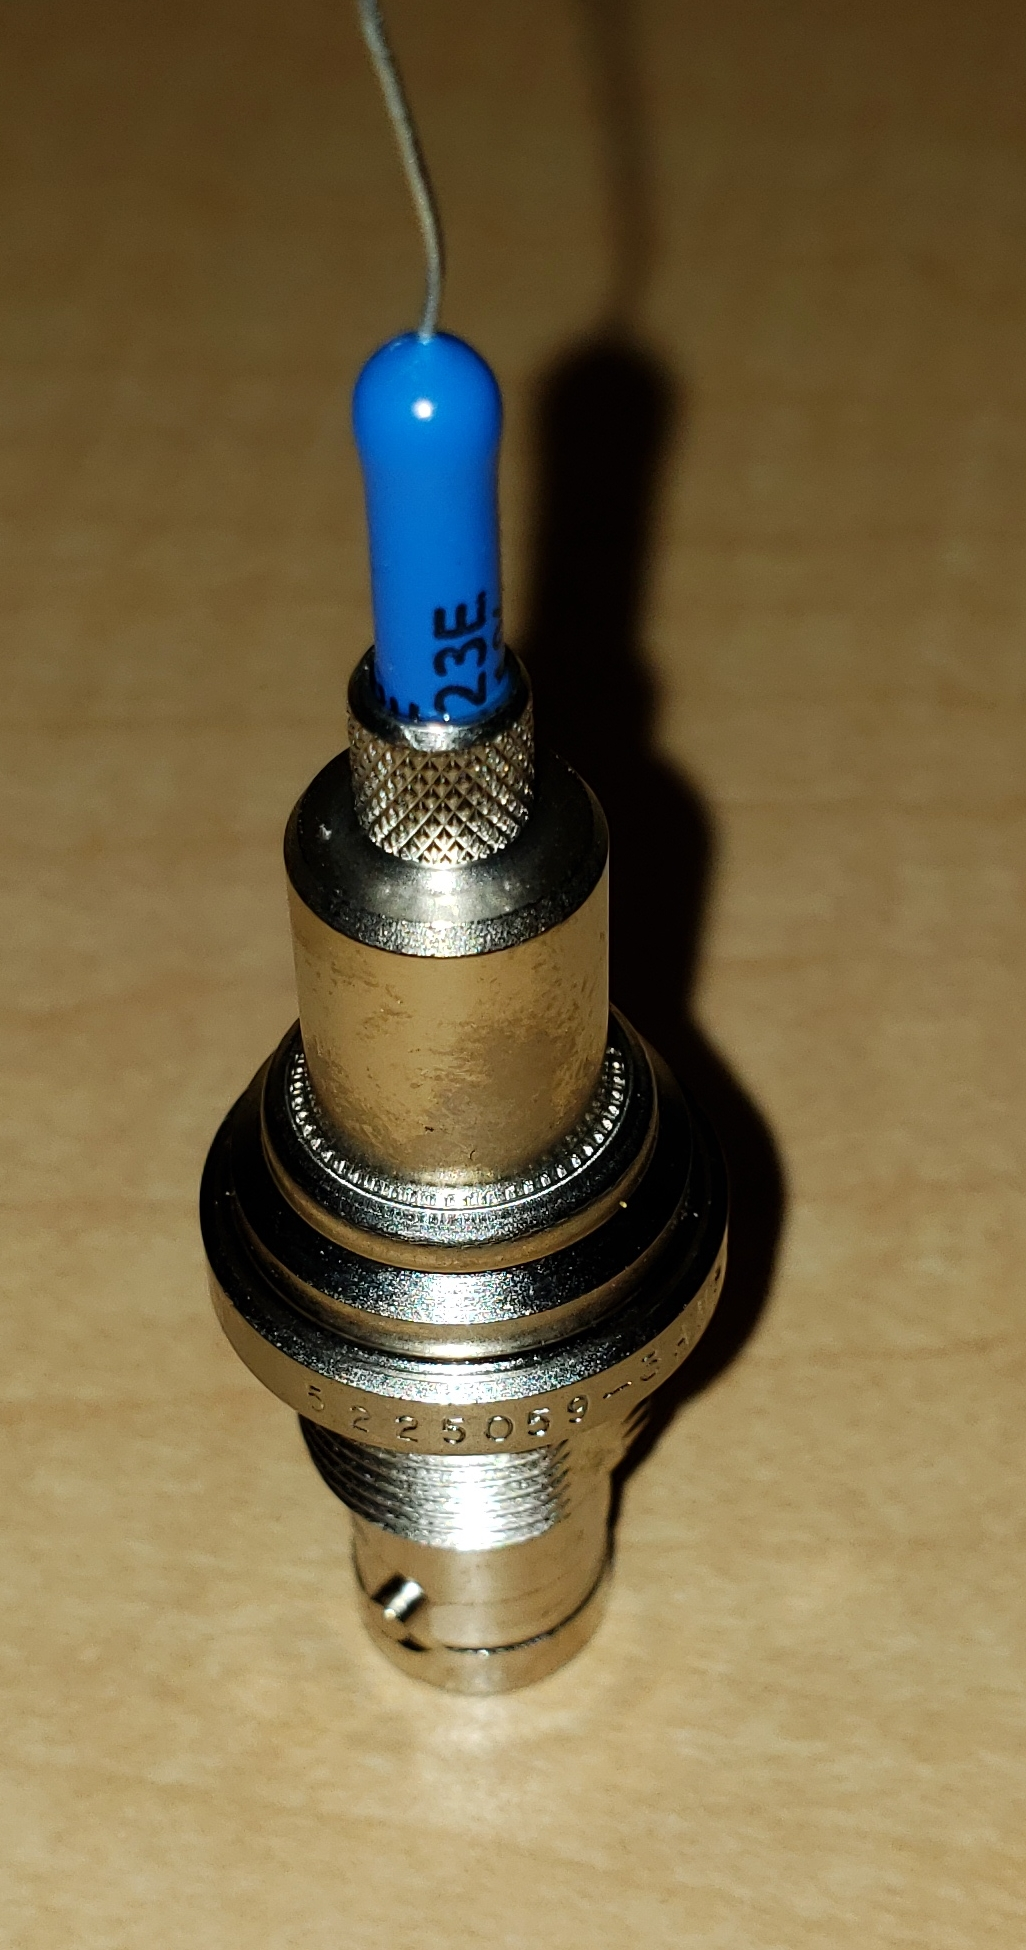
\includegraphics[width=2in]{ResistorInConnector}

\caption{Resistor installed in bulkhead jack.}
\end{figure}


\section{Preparing the tube}
\begin{enumerate}
\item Measure the section of tube using the tube jig and cut to length with
tube cutter. See figure \ref{fig:CuttingTube}.
\begin{figure}[H]
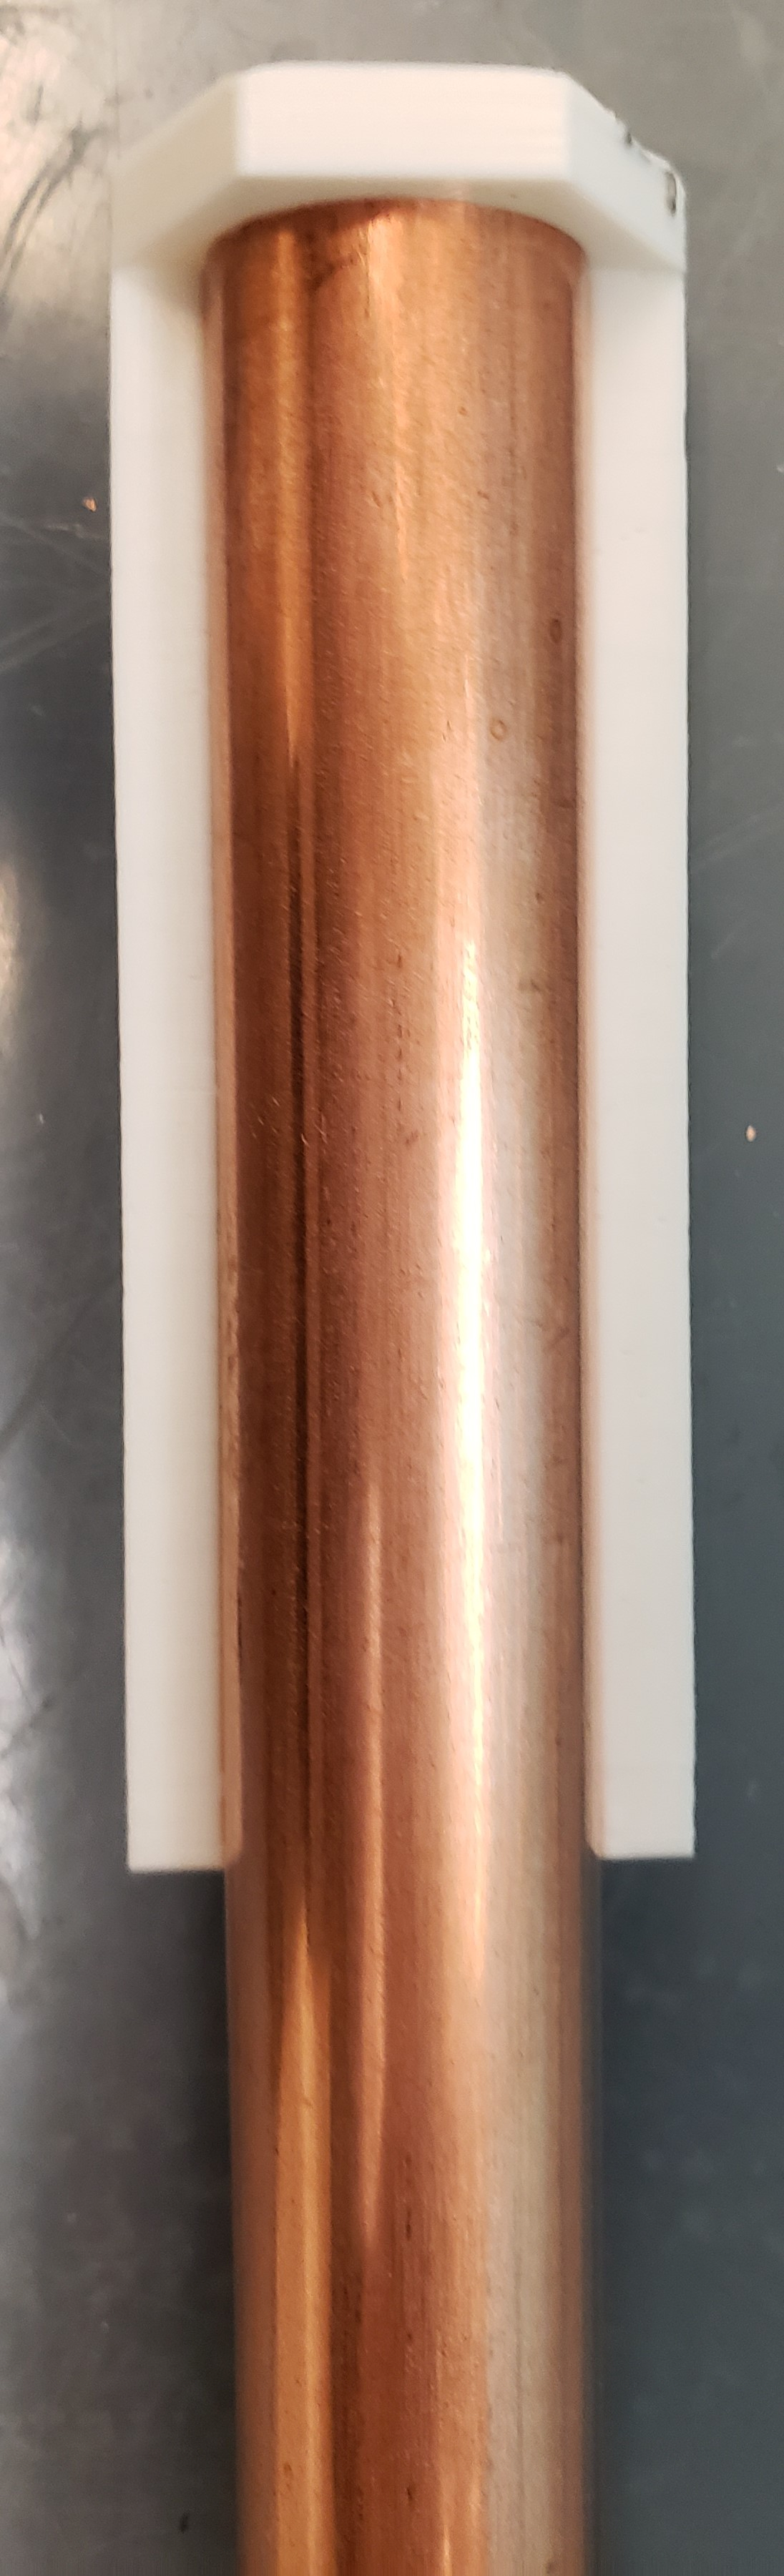
\includegraphics[height=3in]{TubeMeasuredInJig}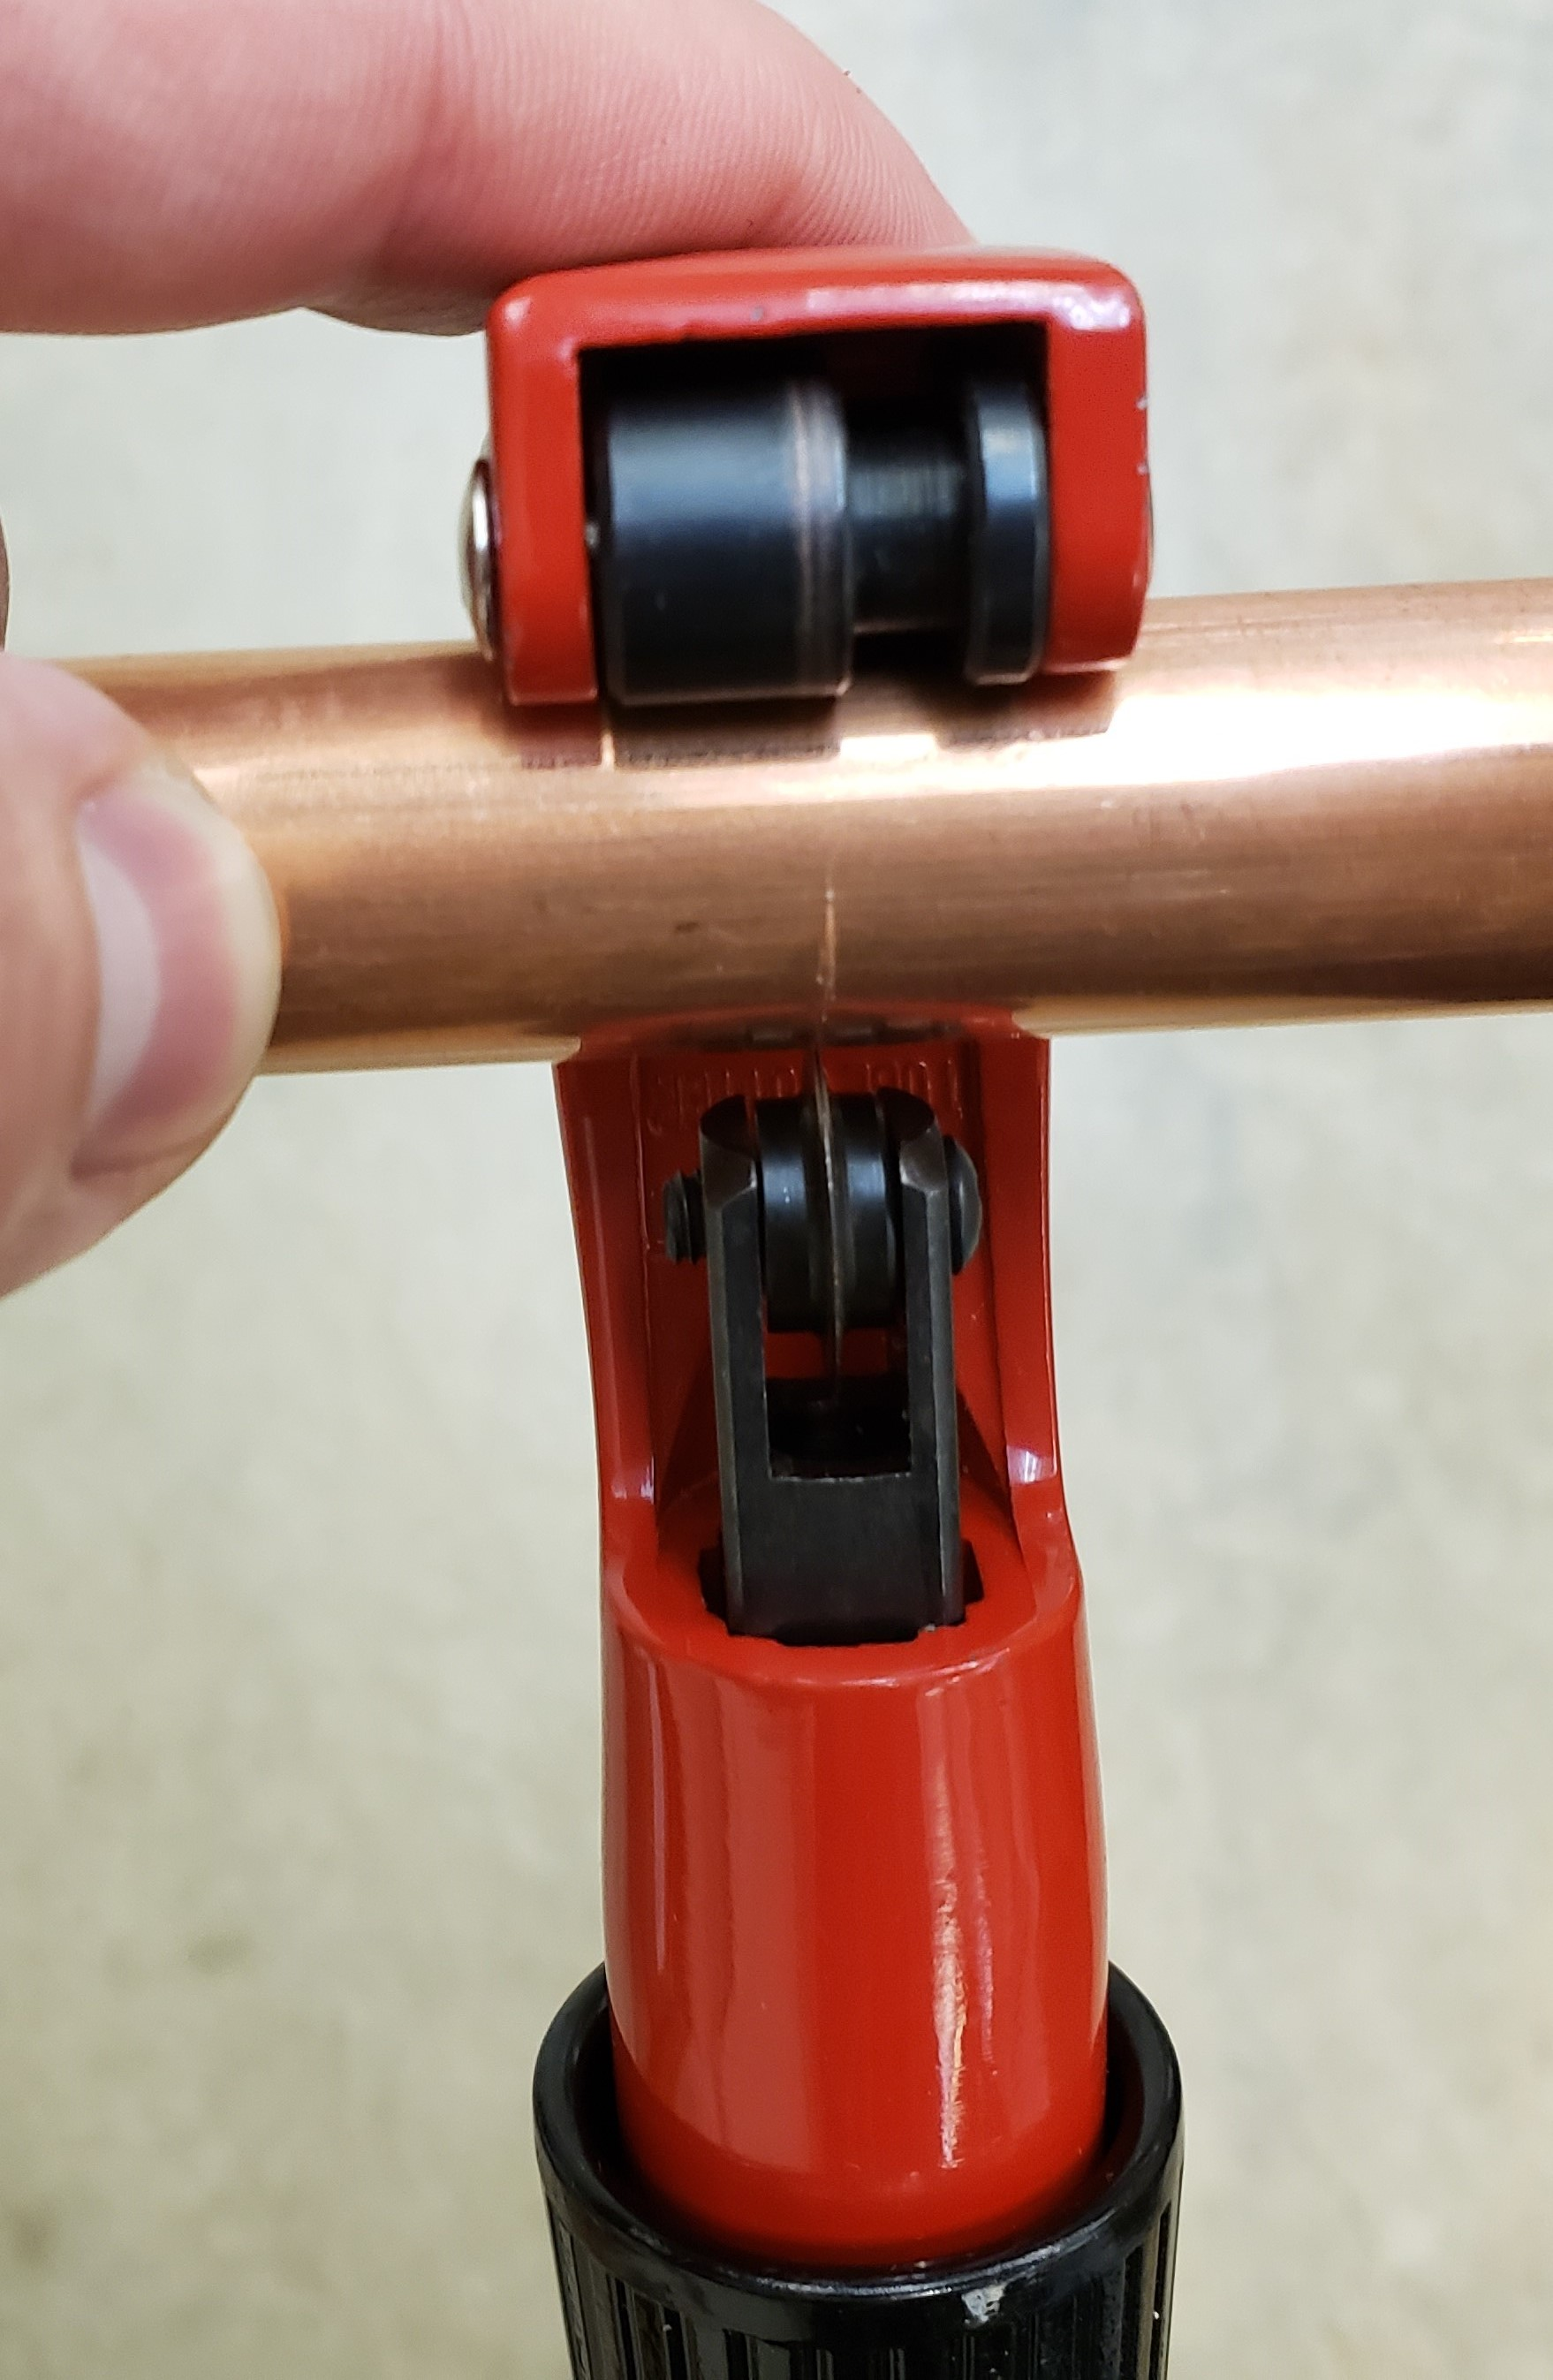
\includegraphics[height=3in]{TubeCutting}\caption{\label{fig:CuttingTube}Left: measuring tube with jig. Right: cutting
tube with tube cutter.}
\end{figure}
\item Place the cut tube in the jig and drill the 3/32'' fill hole and
1/16'' capacitor solder joint holes. The 3/32'' hole is on both
sides of the jig but only one is necessary. All six capacitor holes
are desired for six capacitor, if installing fewer capacitors then
space the holes evenly about the tube. Only install a number of capacitors
that can be spaced such that the radiation to the output from any
current flowing radially through the capacitors will cancel. This
allows two, three, four, or six capacitors but not one or five capacitors.
\begin{figure}[H]
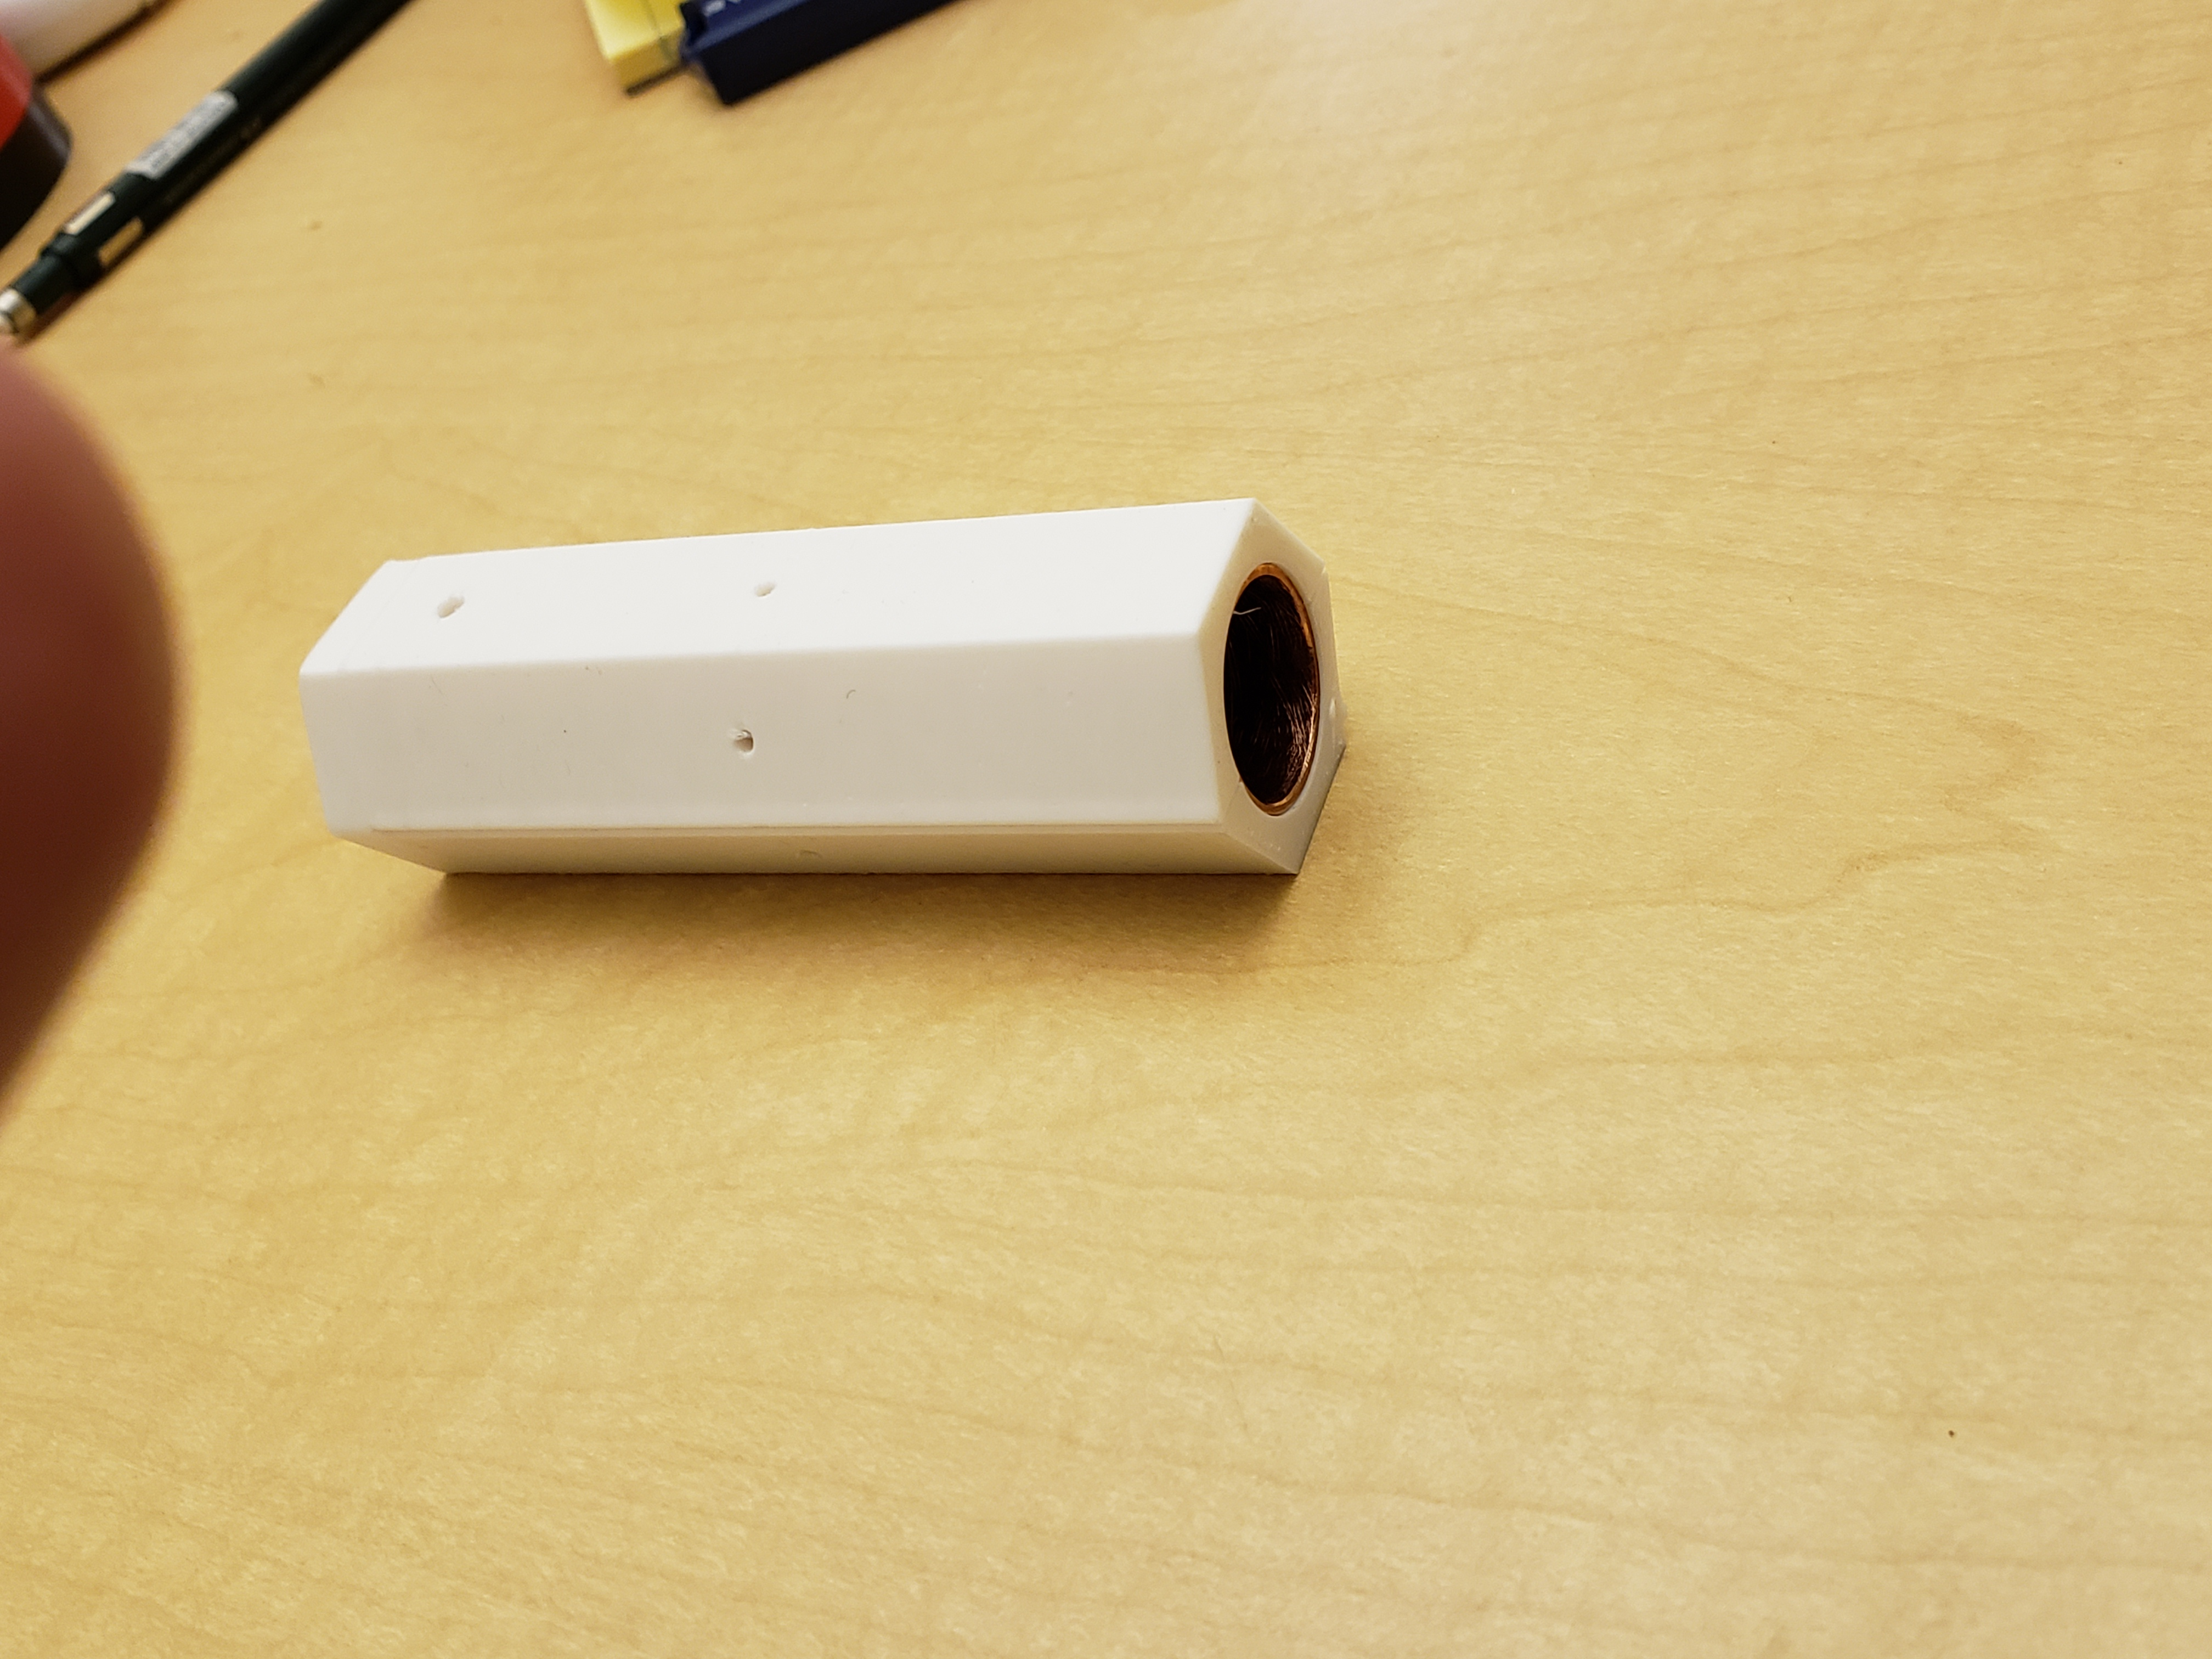
\includegraphics[width=4in]{TubeInJig}

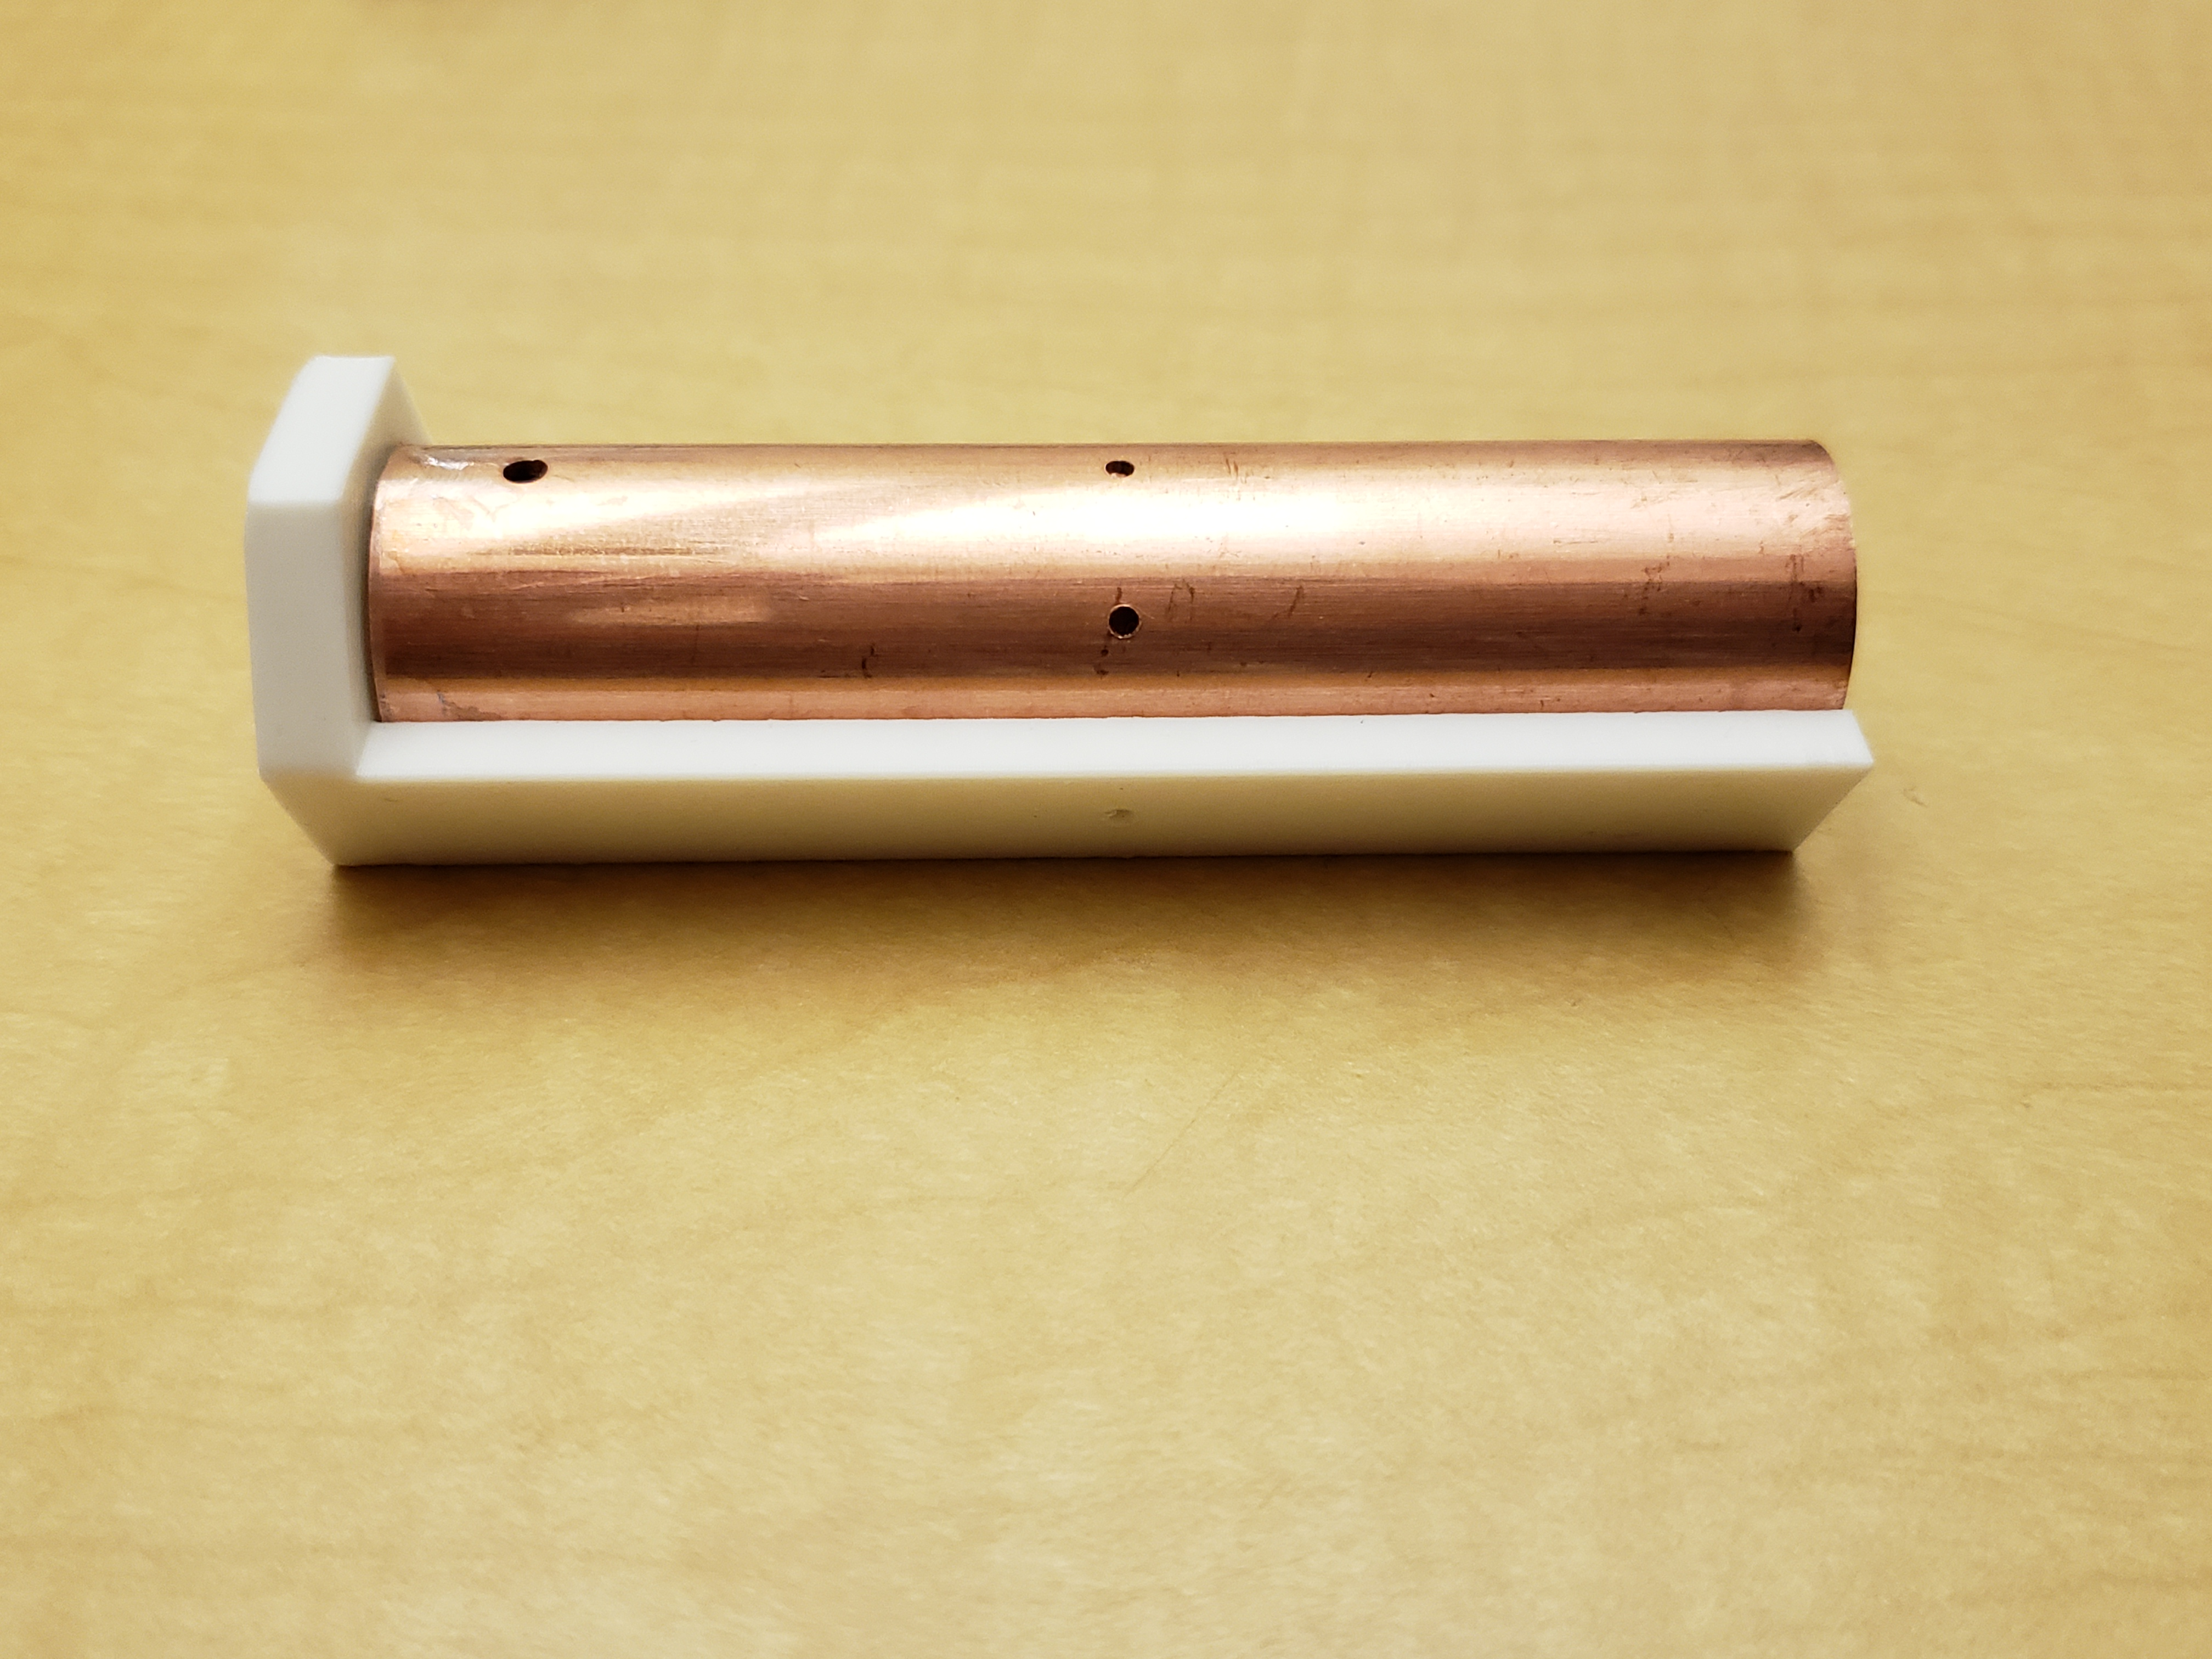
\includegraphics[width=4in]{TubeHolesDrilled}

\caption{\label{fig:TubeHoles}Top: tube in jig ready to be drilled. Bottom:
half of jig removed after drilling holes.}
\end{figure}
\item File any burs off the drill holes, be sure to get the interior side
of the tube as the capacitors will catch on any burs.
\item Test fit the SHV jack in the tube, remember that a small gap is necessary
for solder. The tube will likely need to be bored out, if so it is
helpful to bore to the desired insertion depth so the connector easily
inserts then stops in the desired position. The connector should be
flush with the end of the tube, or slightly less inserted than flush
so that the sealing ring can still be fully compressed. See figure
\ref{fig:PrepareTube}.
\item (Optional) Tin the SHV jack end of the tube in the same manner the
SHV jack was tinned. Check the fit again, if it doesn't go in there's
probably a solder blob that needs to be wicked away.
\begin{figure}[H]
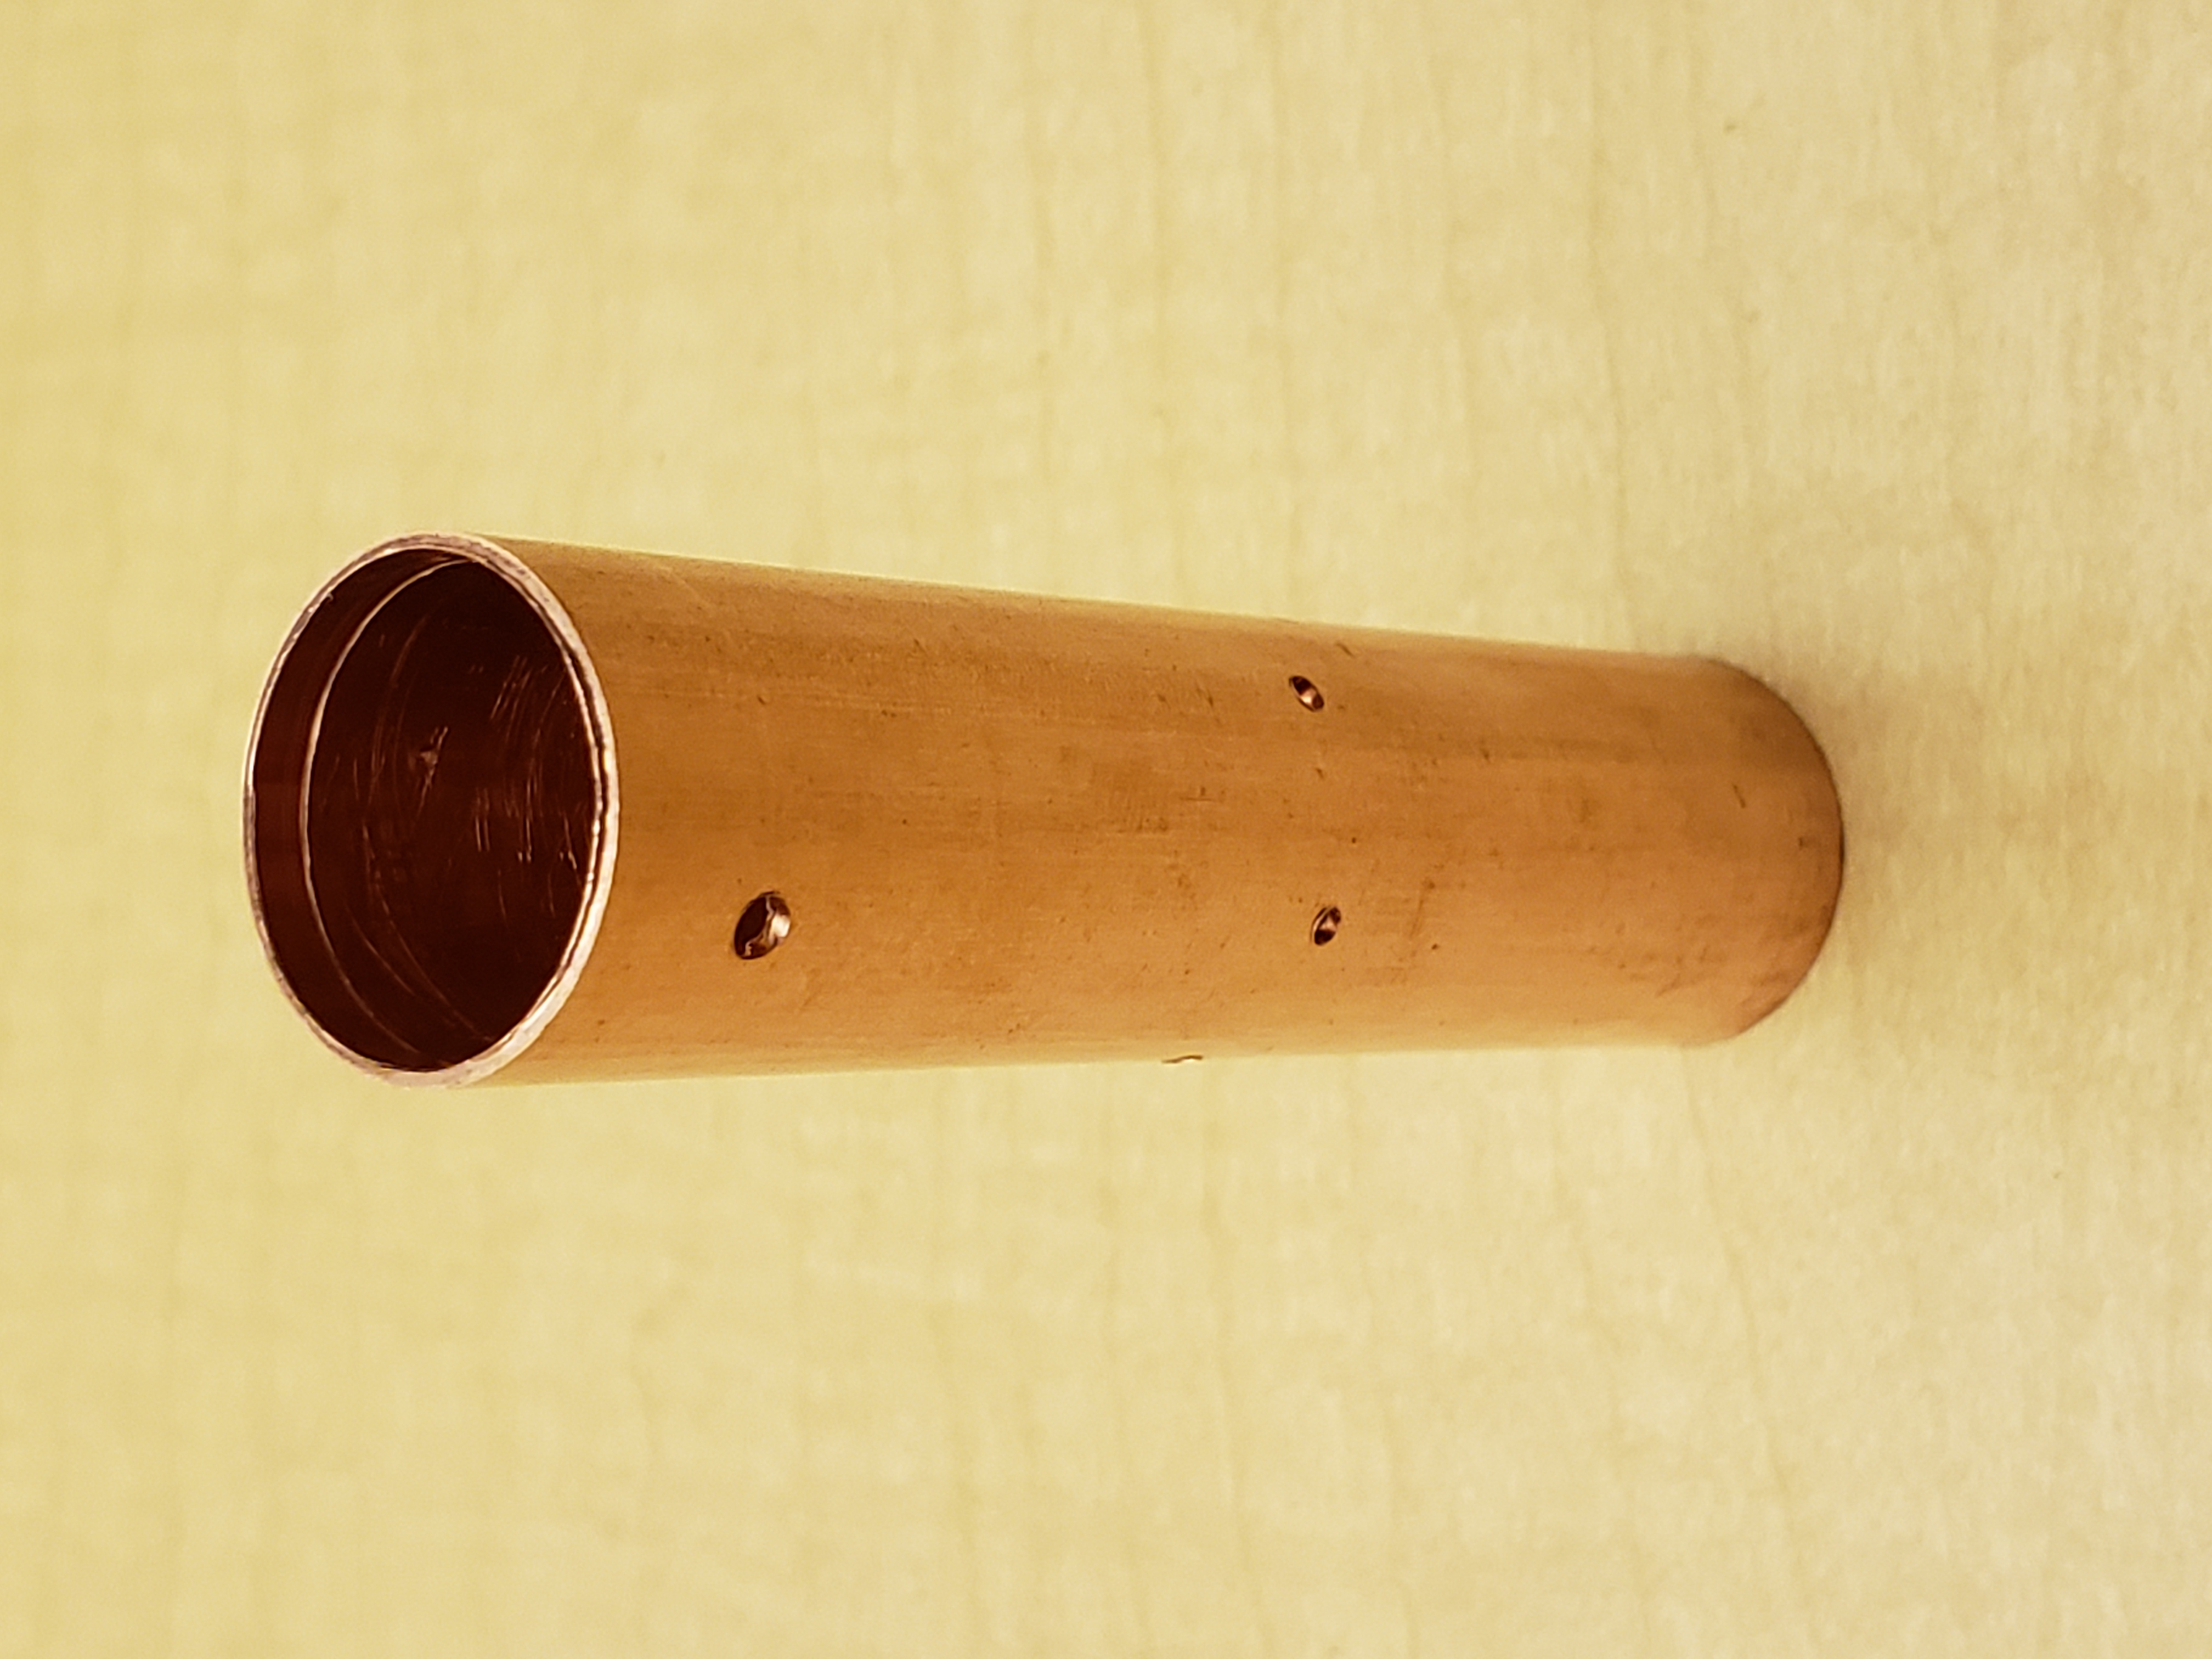
\includegraphics[height=4in]{TubeConnectorEndBored}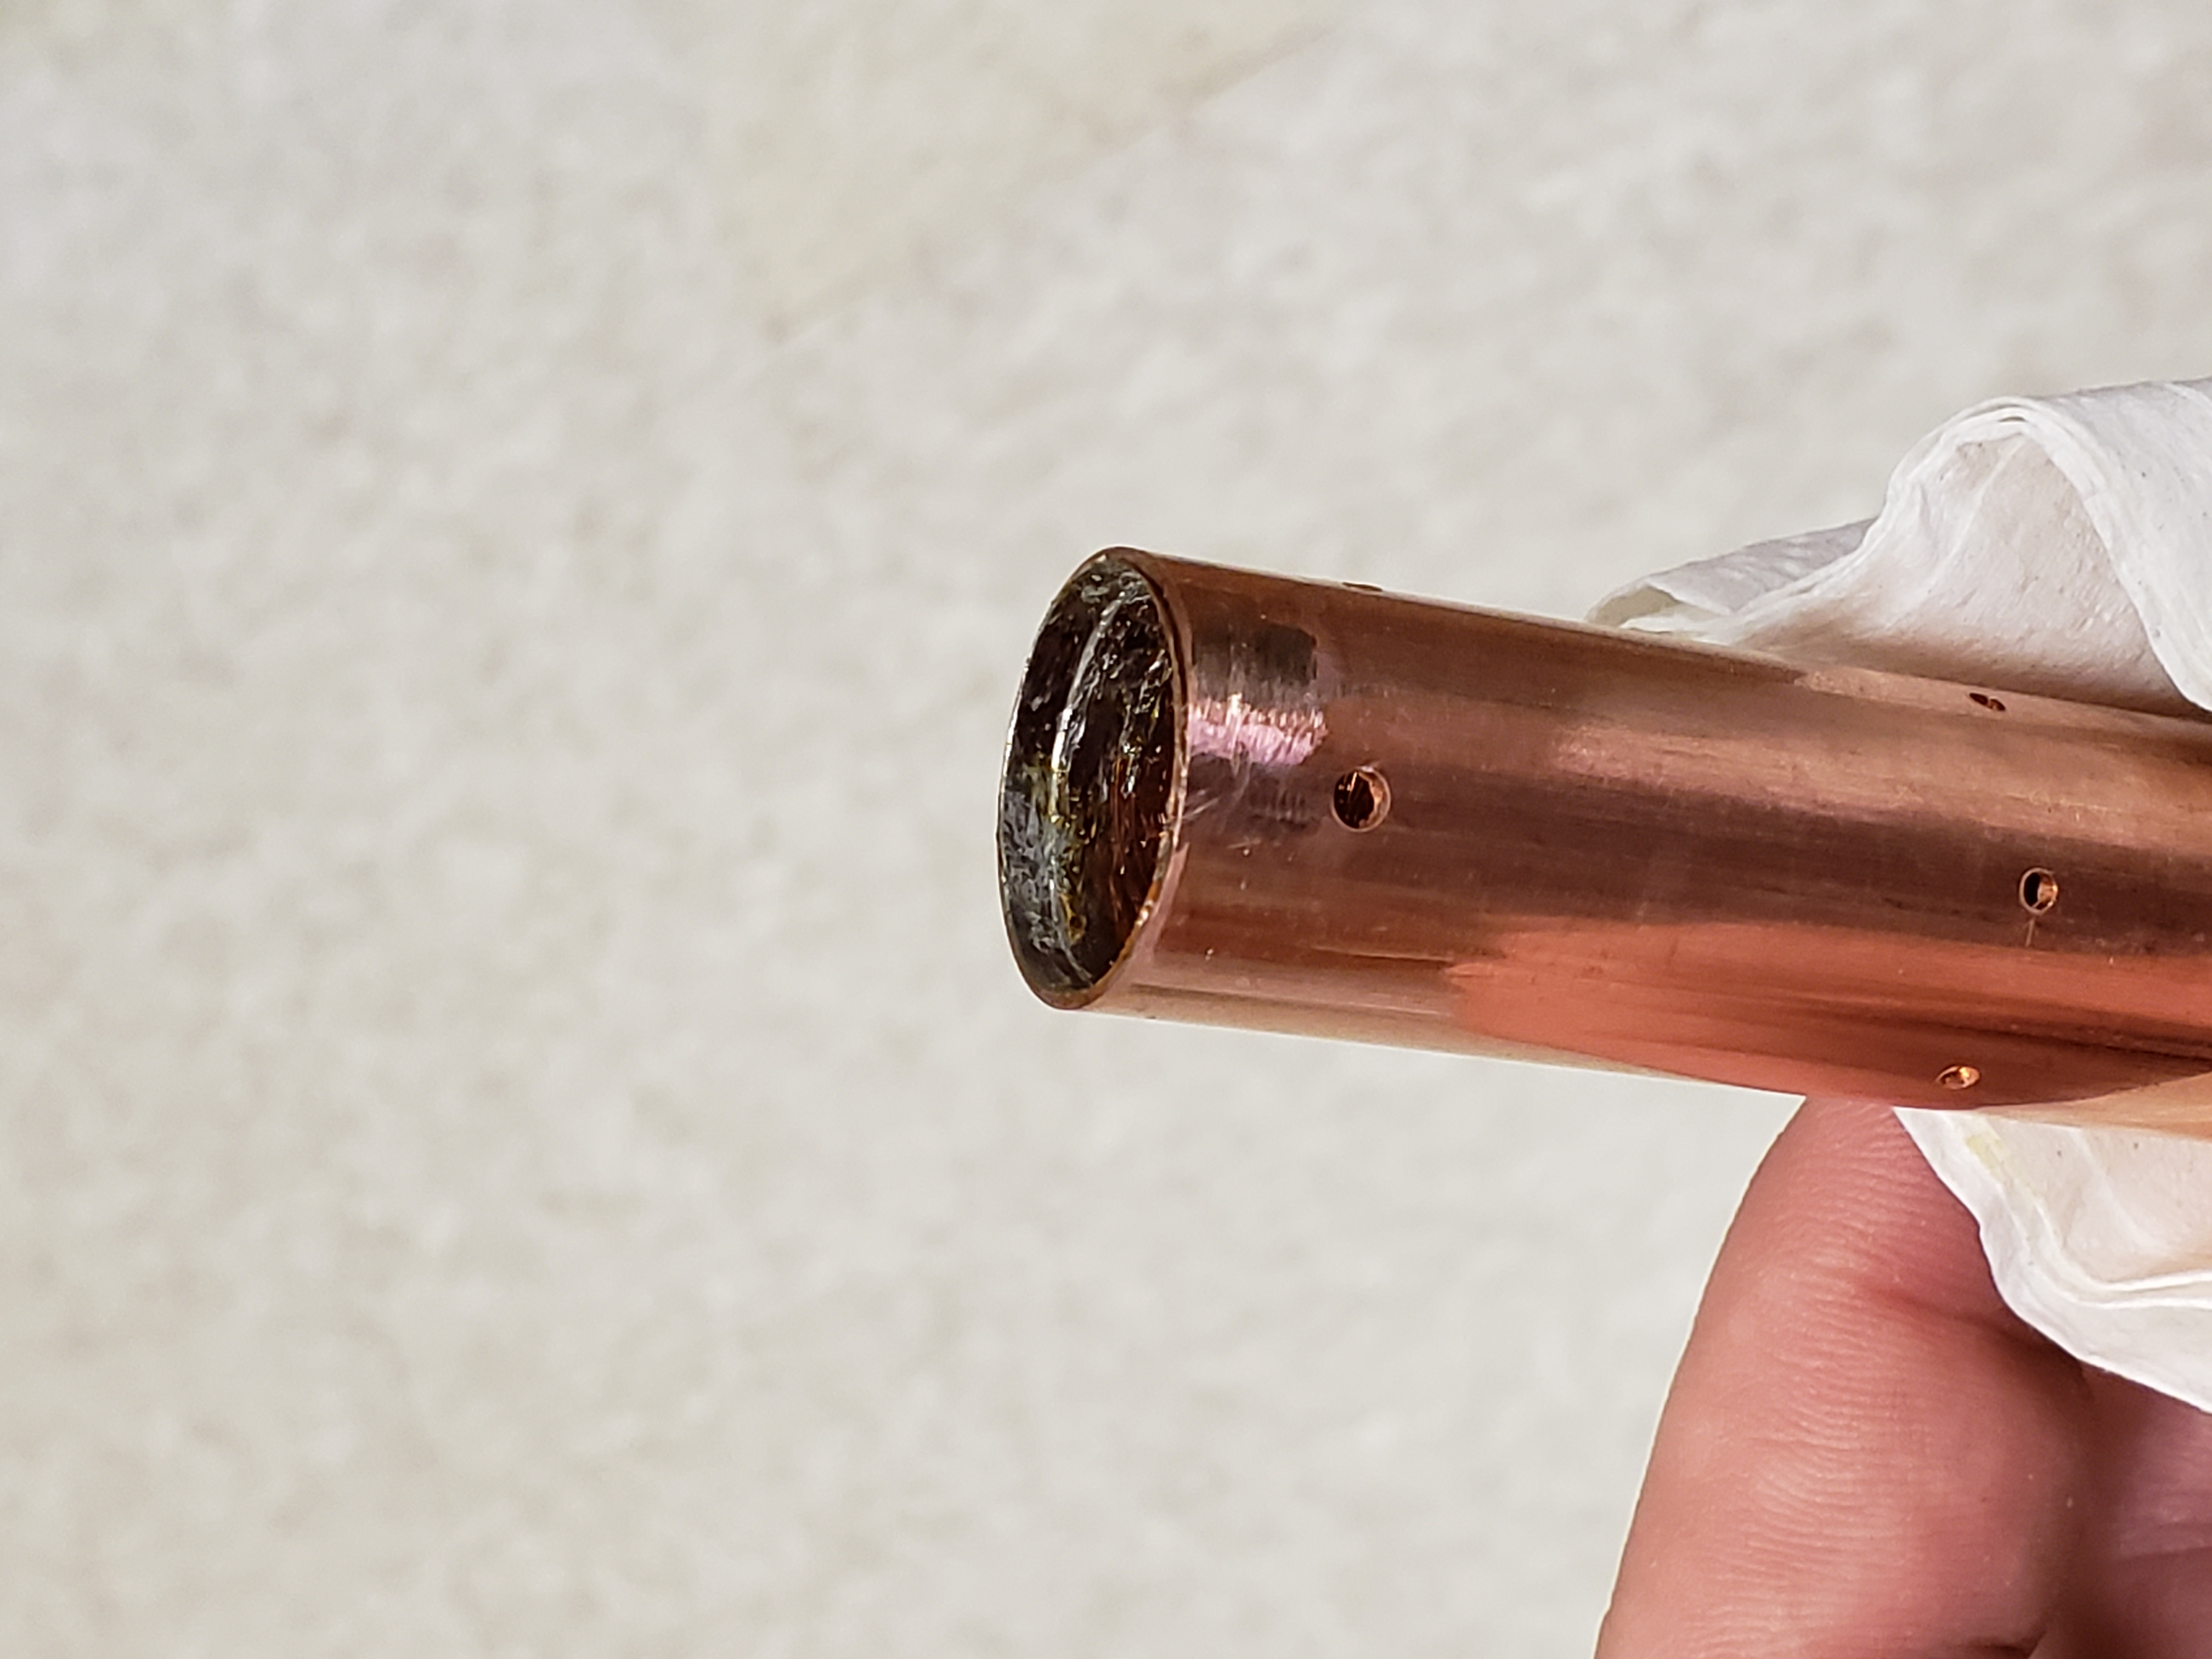
\includegraphics[height=4in]{TubeTinned}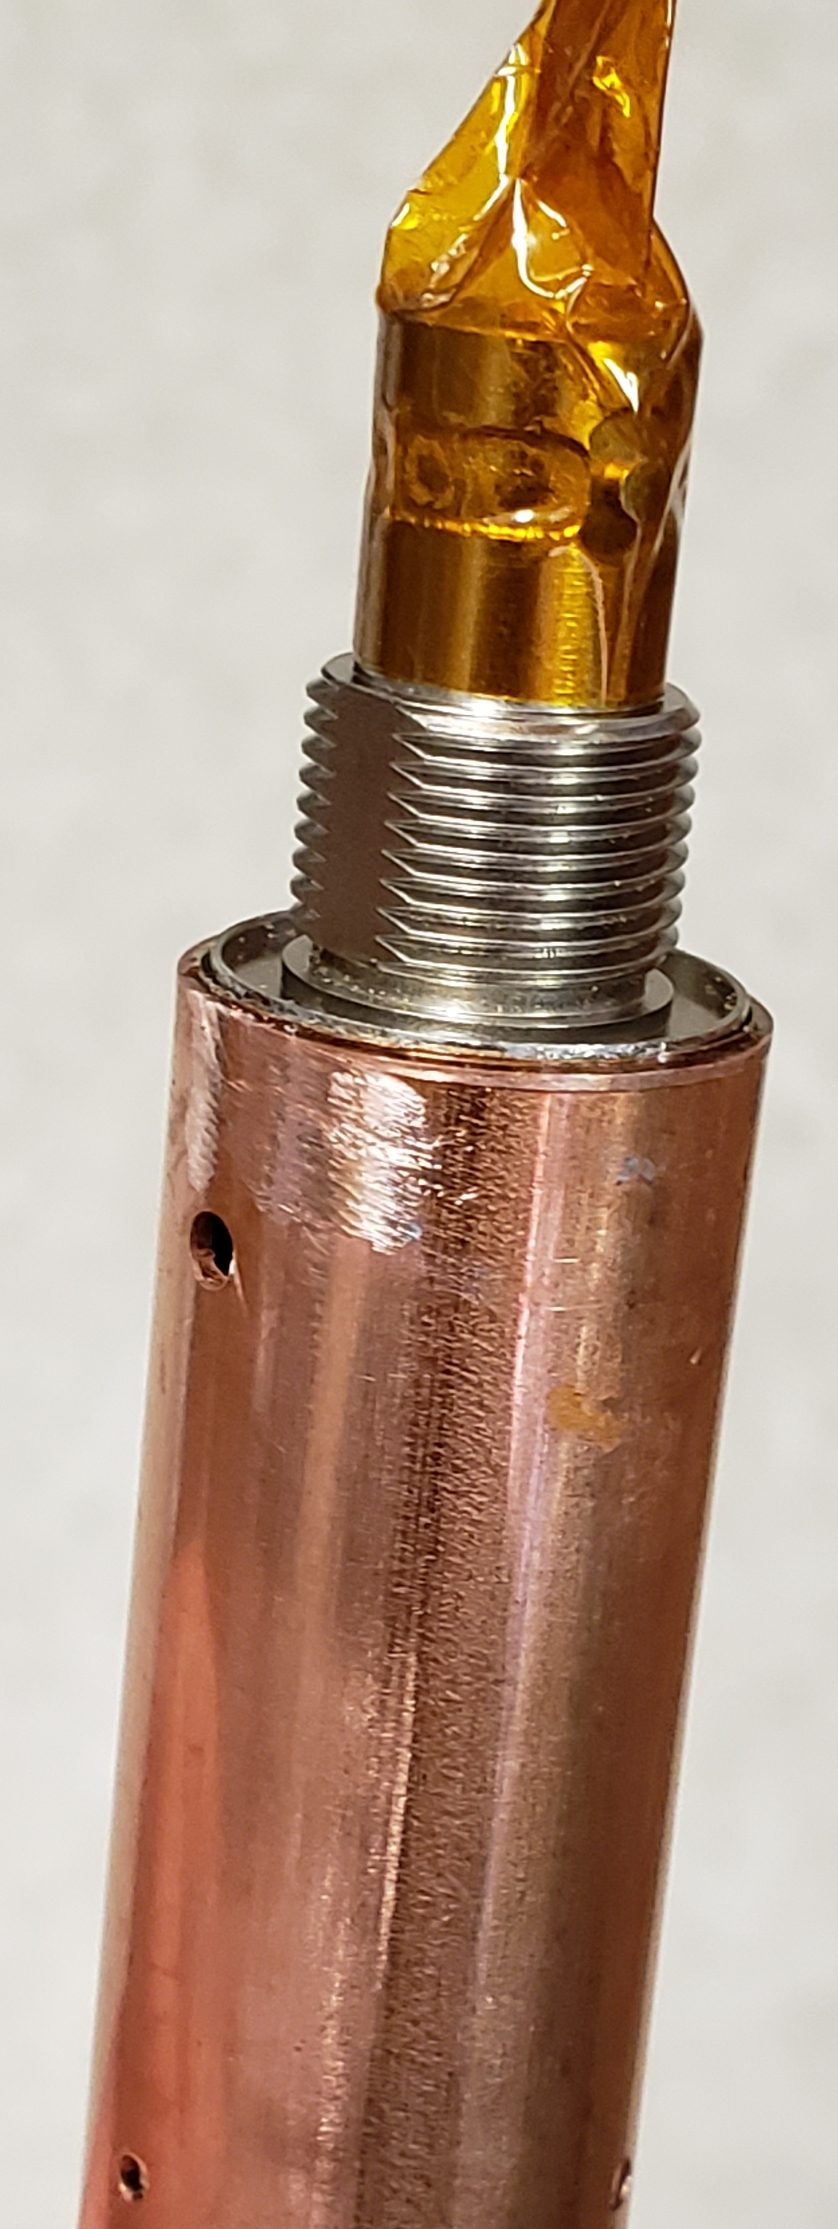
\includegraphics[height=4in]{ConnectAndTubeTestFit}\caption{\label{fig:PrepareTube}Left: tube bored out to allow connector to
fit. Center: tinned tube. Right: connector resting on shoulder in
bored out tube.}
\end{figure}
\item Solder the washer to the cable end of the tube. For the chosen washer
and tube it should be a press fit. If it can't fit into the tube it
can be soldered over the end, if it falls through it can be secured
with Kapton tape to hold in place during initial soldering. The cable
shield will be soldered here later so a large solder excess is fine.
Make sure all gaps between the tube and washer are sealed as this
is an oil boundry.
\begin{figure}[H]

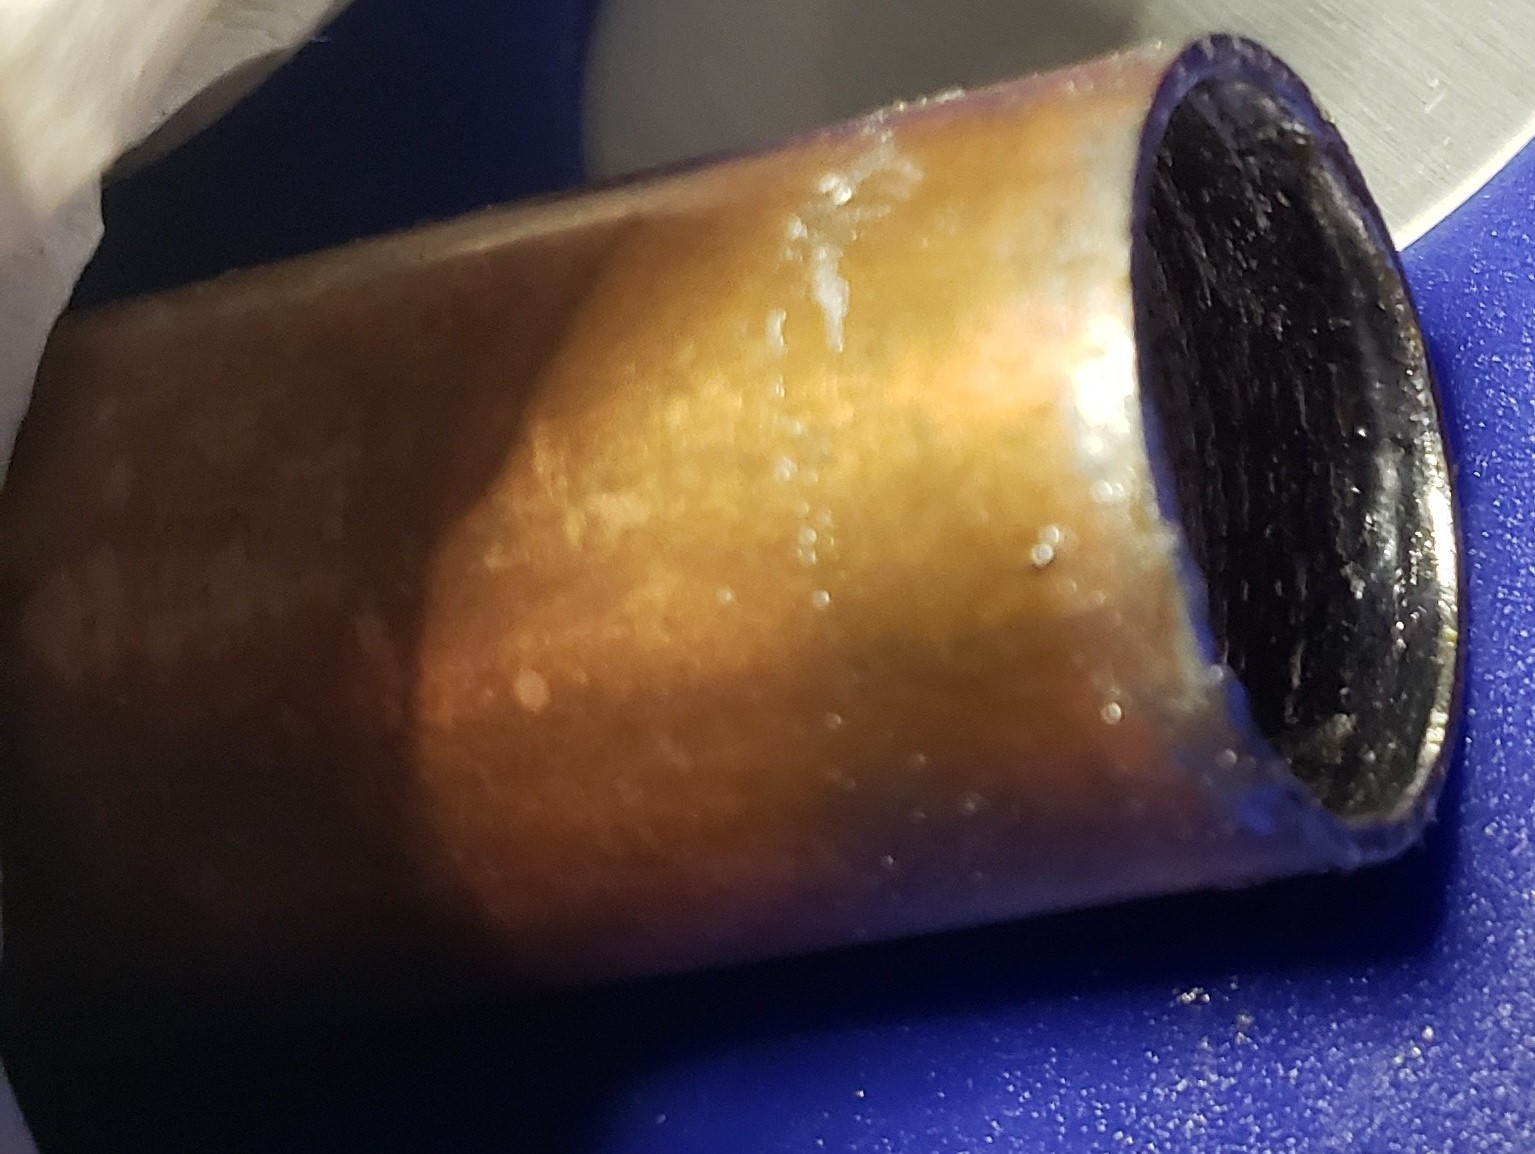
\includegraphics[angle=90,height=4in]{TubeCableEndTinned}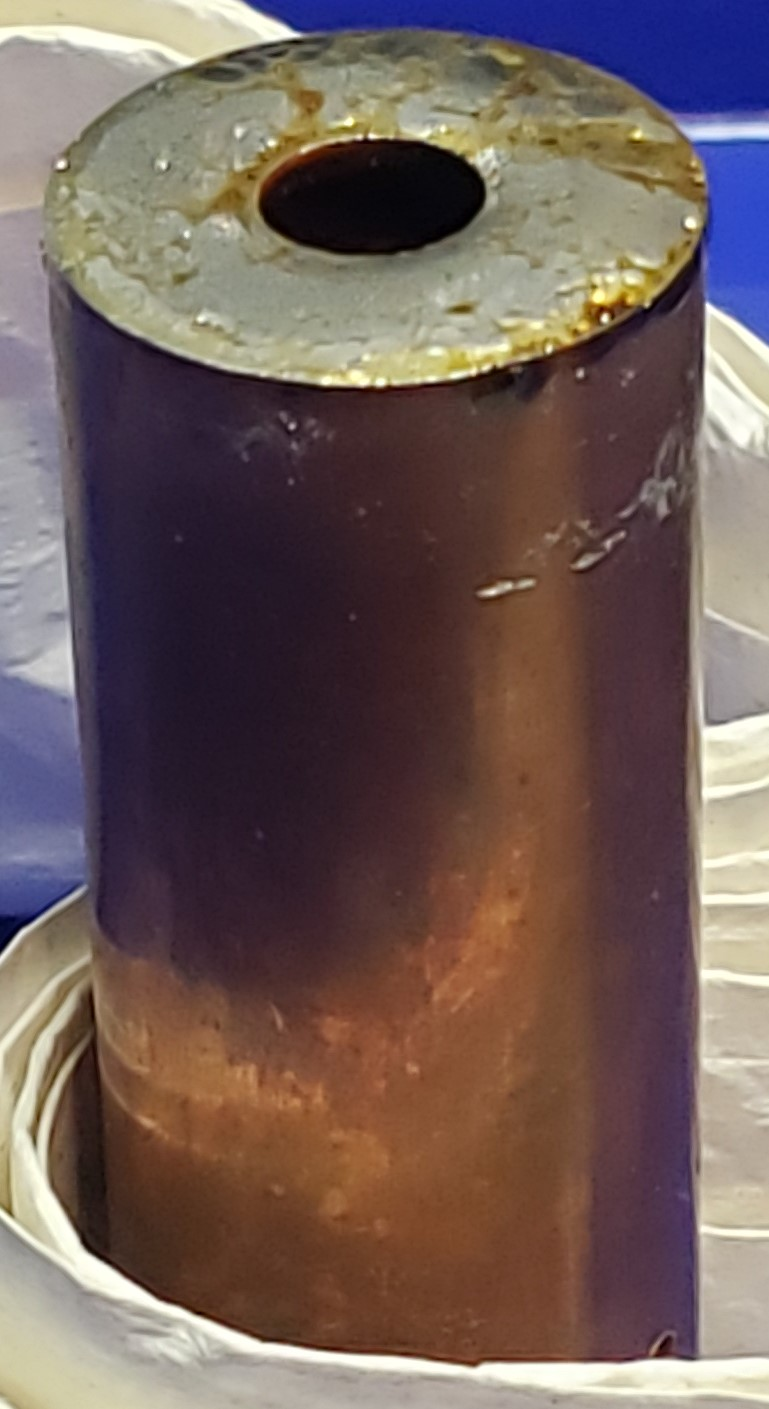
\includegraphics[height=4in]{TubeWasherInstalled}\caption{Left: cable end of tube tinned for a press fit washer. Right: washer
installed in cable end of tube.}
\end{figure}
\end{enumerate}

\section{Assemble the resistors and capacitors}

\subsection{Assemble the capacitors}
\begin{enumerate}
\item Place the capacitors and standoff in the jig. If using a 5 mm standoff
place an M2.5 washer under the standoff for a spacer. Lightly tighten
the bolts to hold the capacitors in place. The spring in the plastic
jig will push the capacitors fully against the standoff when soldering
without requiring significant deflection. Once tight, remove the washer.
\item Test fit the capacitors to ensure they can be inserted in the tube,
they will protrude slightly from one side of the jig. Some filing
of the standoff or tube may be necessary. \textbf{Do not file the
resistors.}
\item Heat the standoff while applying additional solder to the capacitor
to standoff joint until the solder flows. Then apply sufficient solder
to fill the center of the standoff. Solder should flow along all the
capacitors while spreading around the standoff.
\begin{figure}[H]
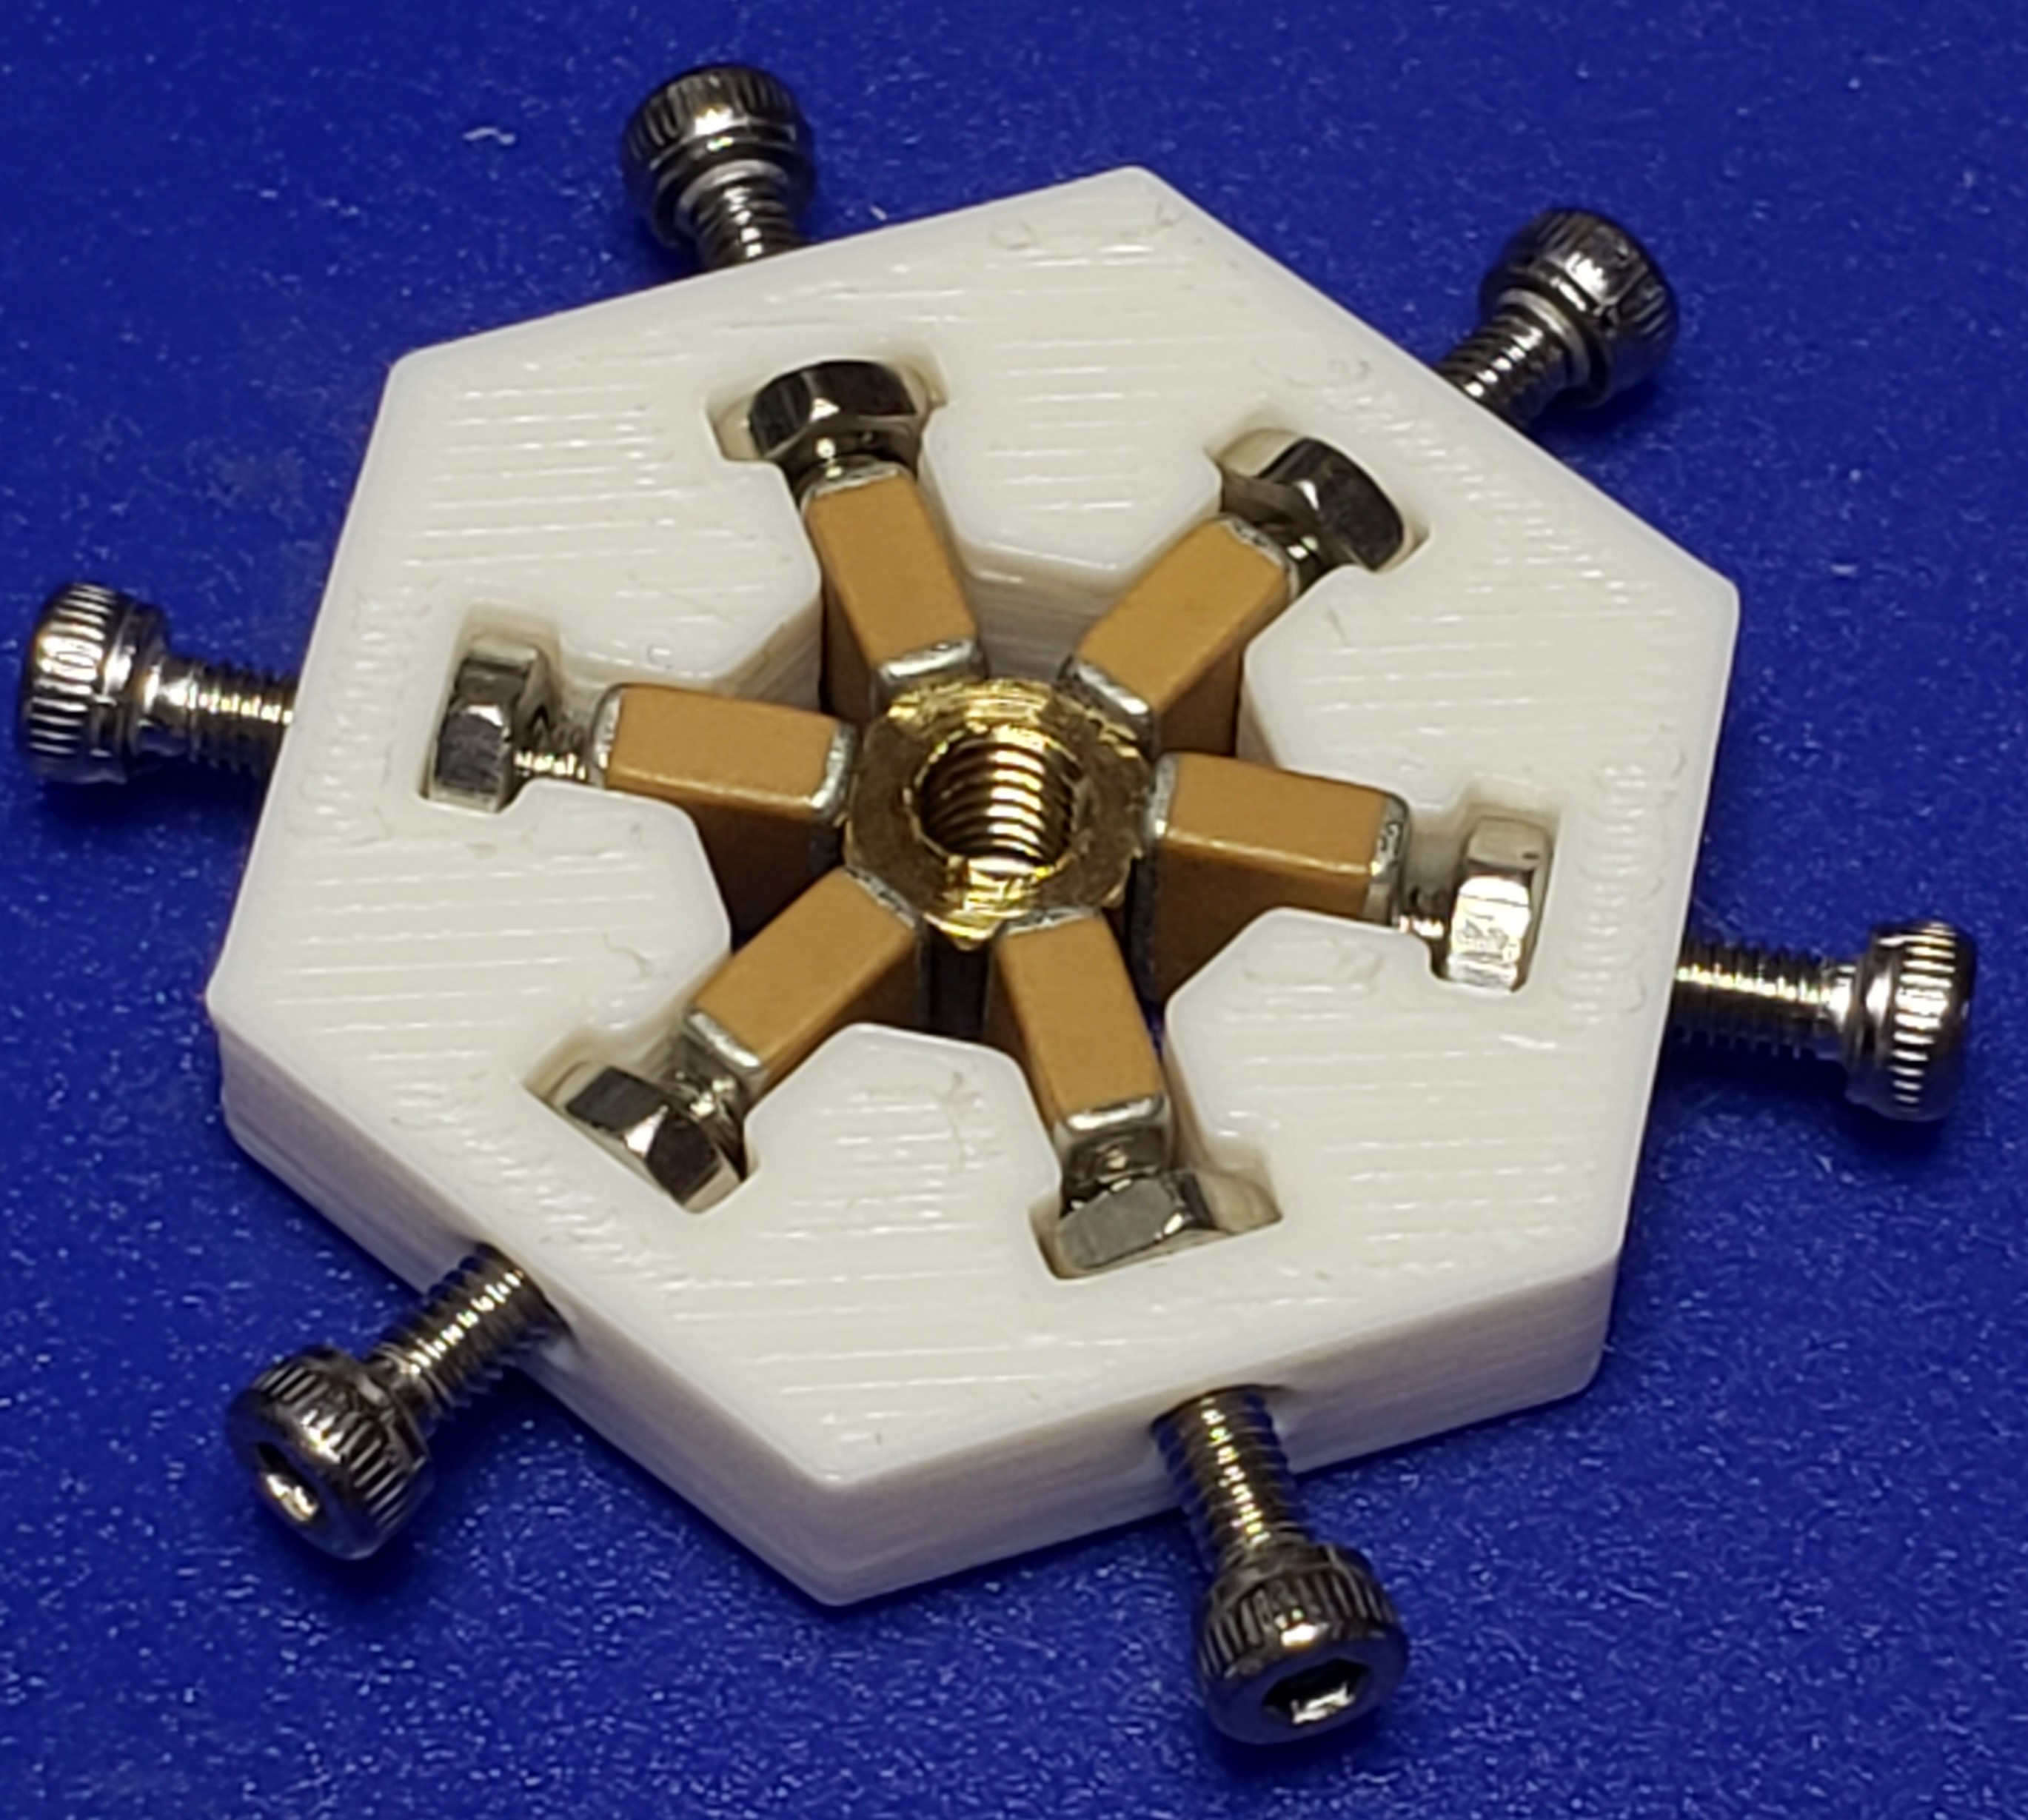
\includegraphics[height=3in]{CapacitorsInJig}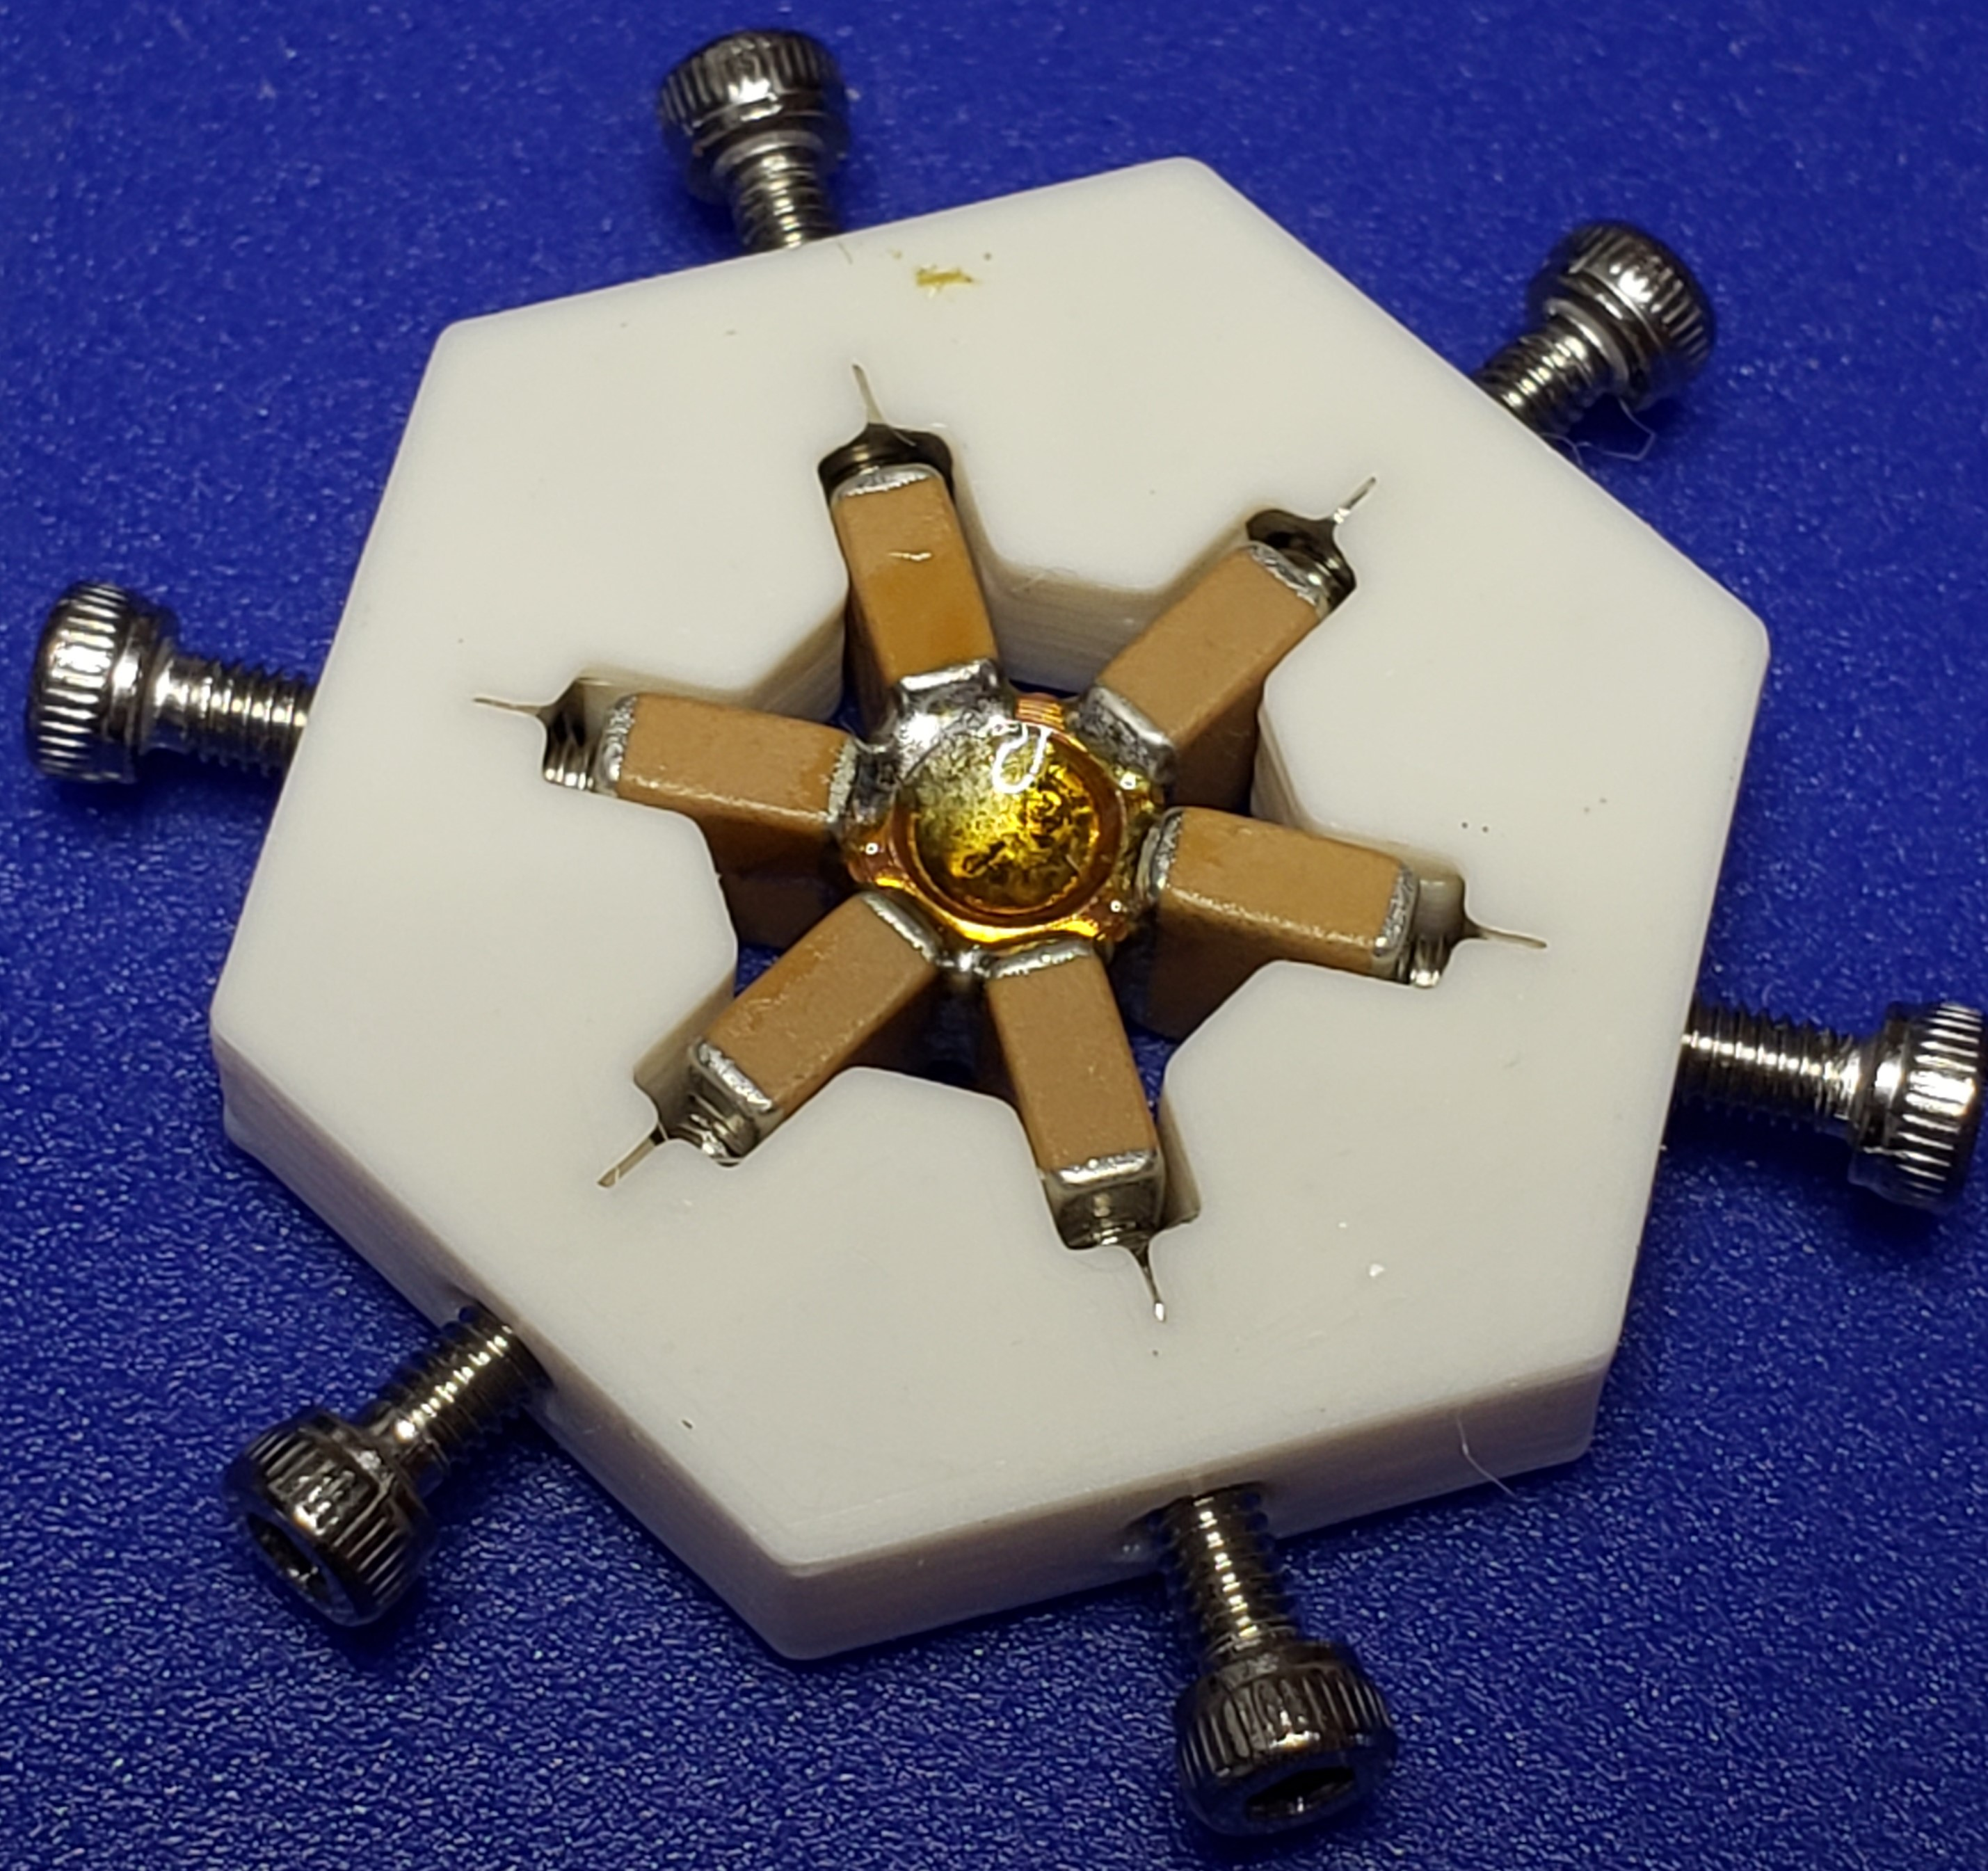
\includegraphics[height=3in]{CapacitorsSolderedInJig}

\caption{Left: capacitors and standoff in jig before soldering. Right: bottom
of capacitors and standoff in jig after woldering, showing the solder
flowed along the standoff to connect all along the capacitors.}
\end{figure}
\item Take the capacitors out of the jig and make sure the can slide into
position in the tube. It is likely some filing of the tube will be
required.
\item Place the capacitors back in the jig to keep them assembled while
soldering the resistors.
\end{enumerate}

\subsection{Asemble the SHV jack, resistors, and capacitors}

\textbf{Don't start this step unless the epoxy used to seal the SHV
jack center pin is cured enough to handle.}
\begin{enumerate}
\item Trim the resistor leads that will go in the standoff down to less
than the standoff length, leaving at least a couple millimeteres for
a solder connection. The leads can be bent so they miss each other
in the hole.
\item Solder the resistor lead from the SHV jack and resistor into the center
of the standoff. Try to keep the resistors well centered, good alignment
will minimize the radiative energy transfer bypassing the filter. 
\item Support the SHV jack, resistor, and capacitors assembly by resting
it on the SHV jack. Support the assembly with a wide part with a hole
to help keep it from tipping.
\item Solder the output resistor lead into the center of the standoff.
\item Remove any solder flux.
\begin{figure}[H]
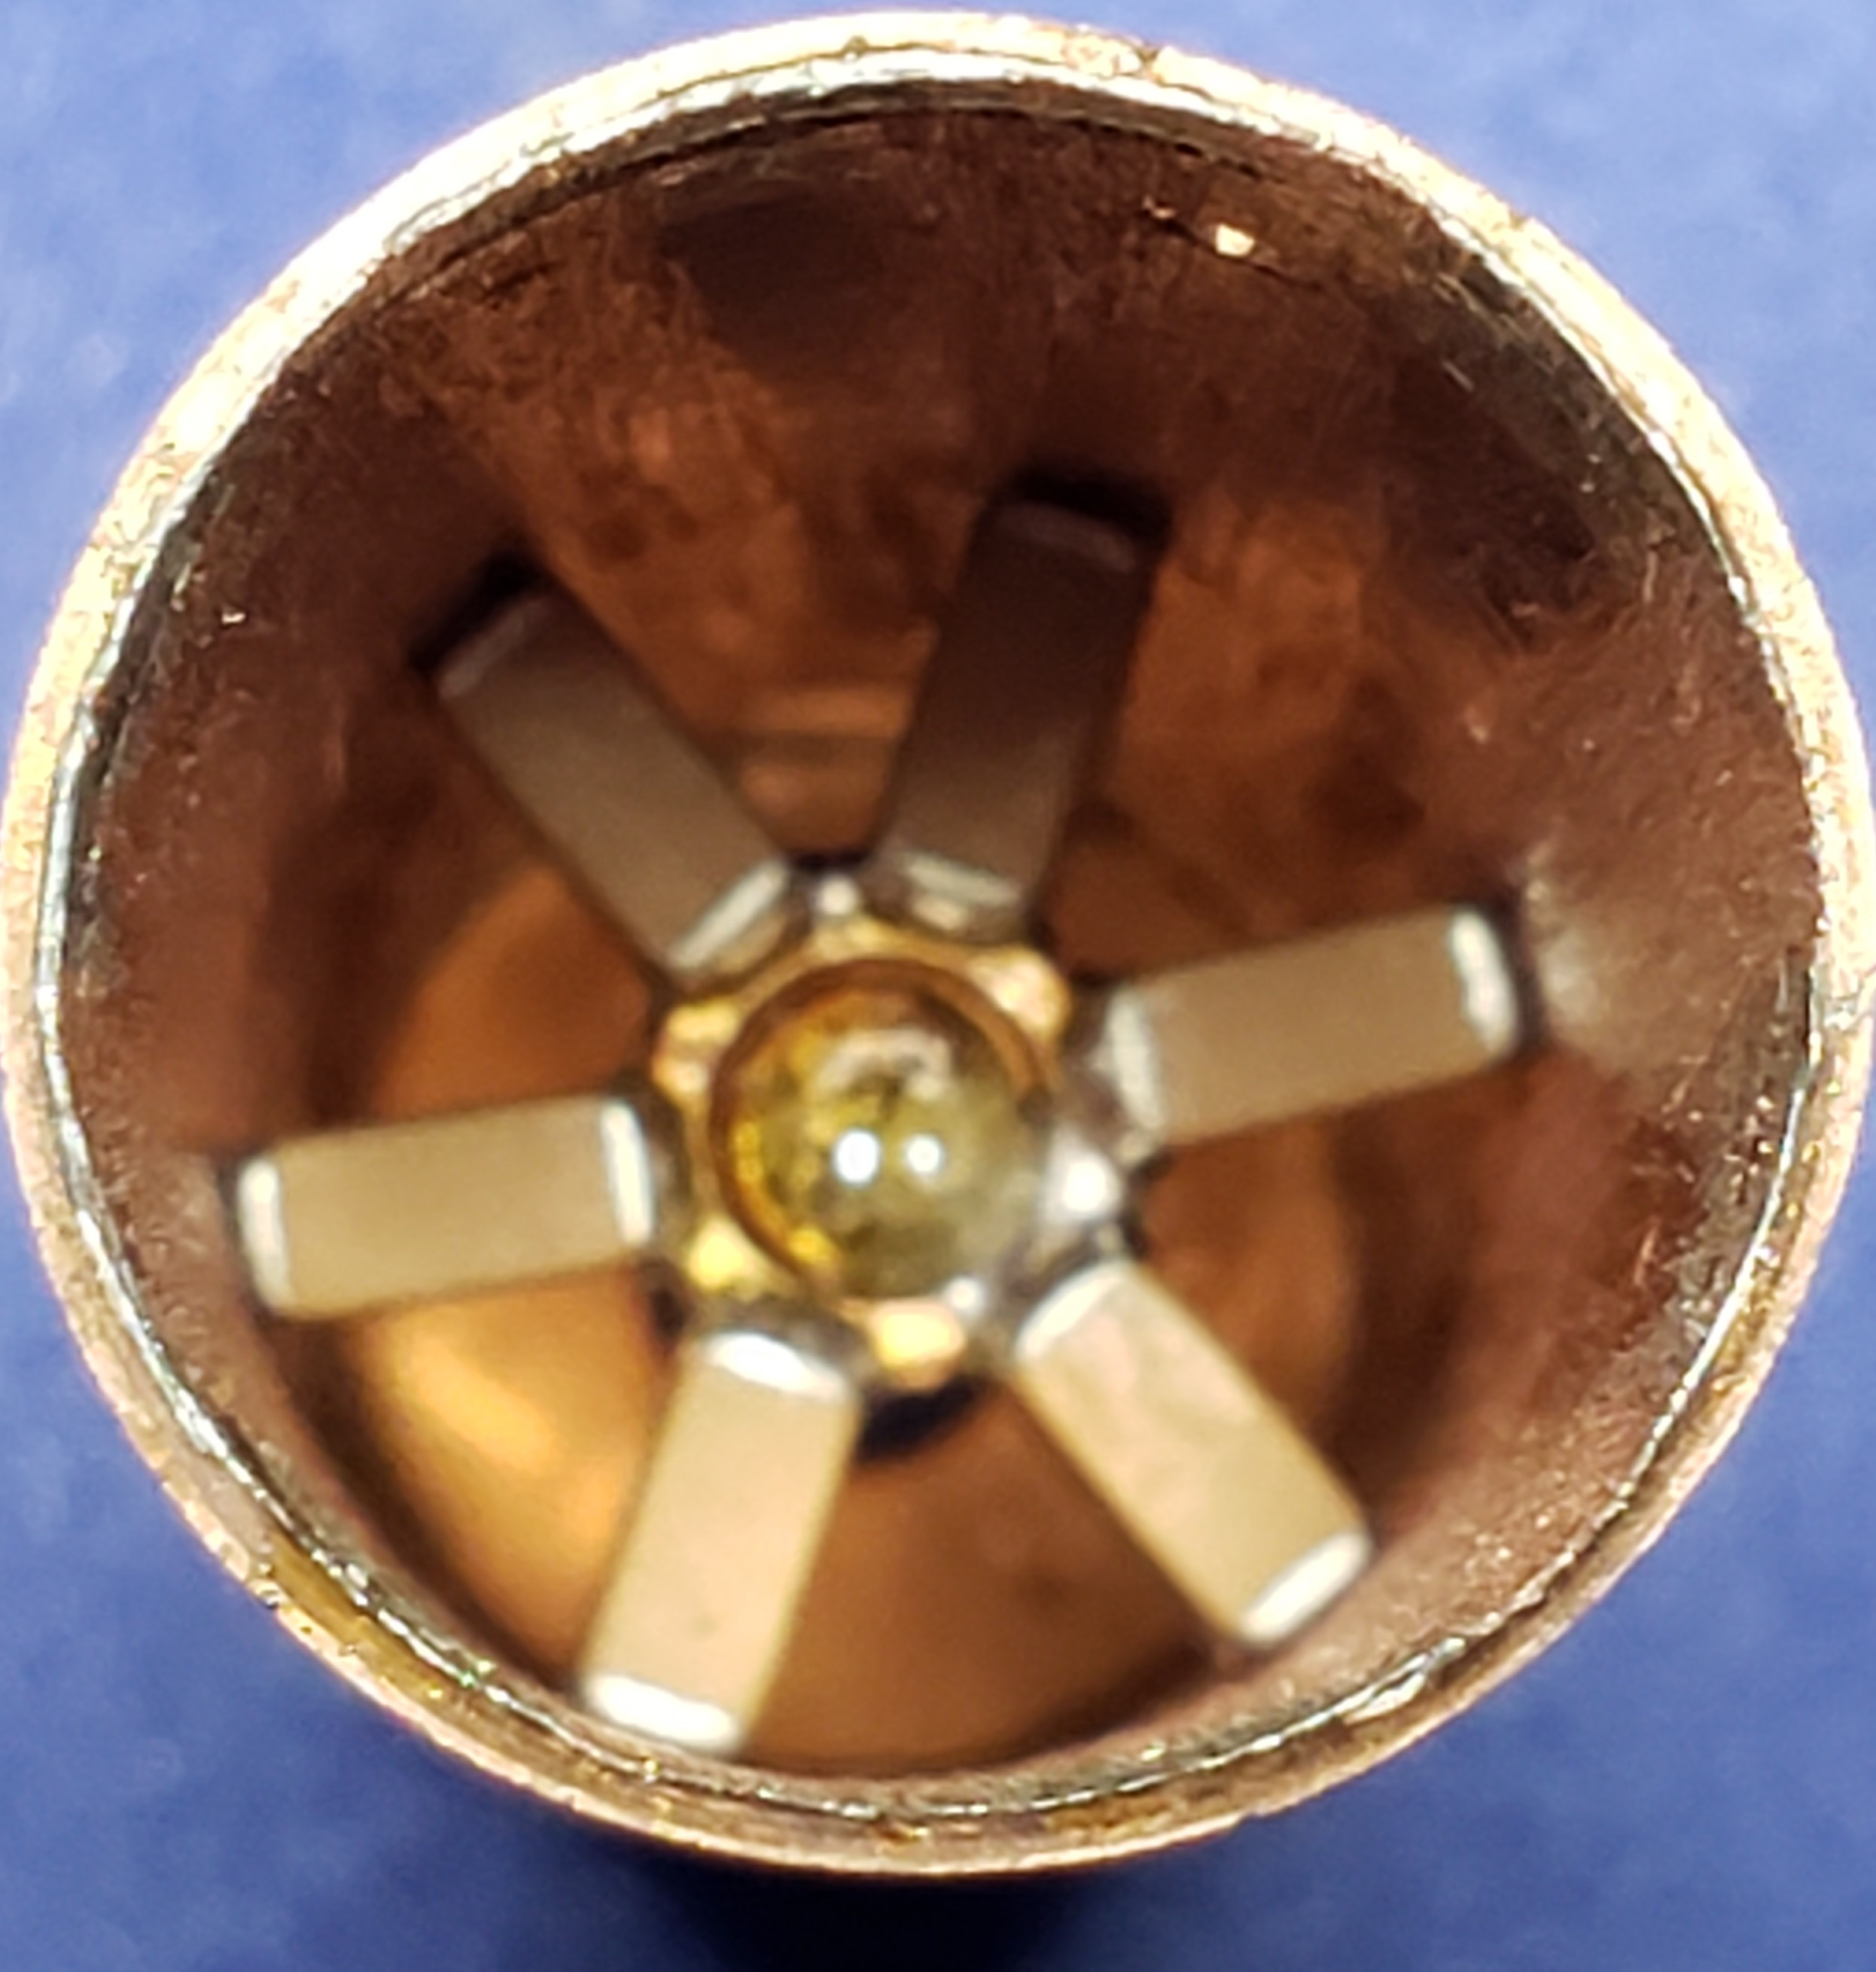
\includegraphics[height=3in]{CapacitorsTestFit}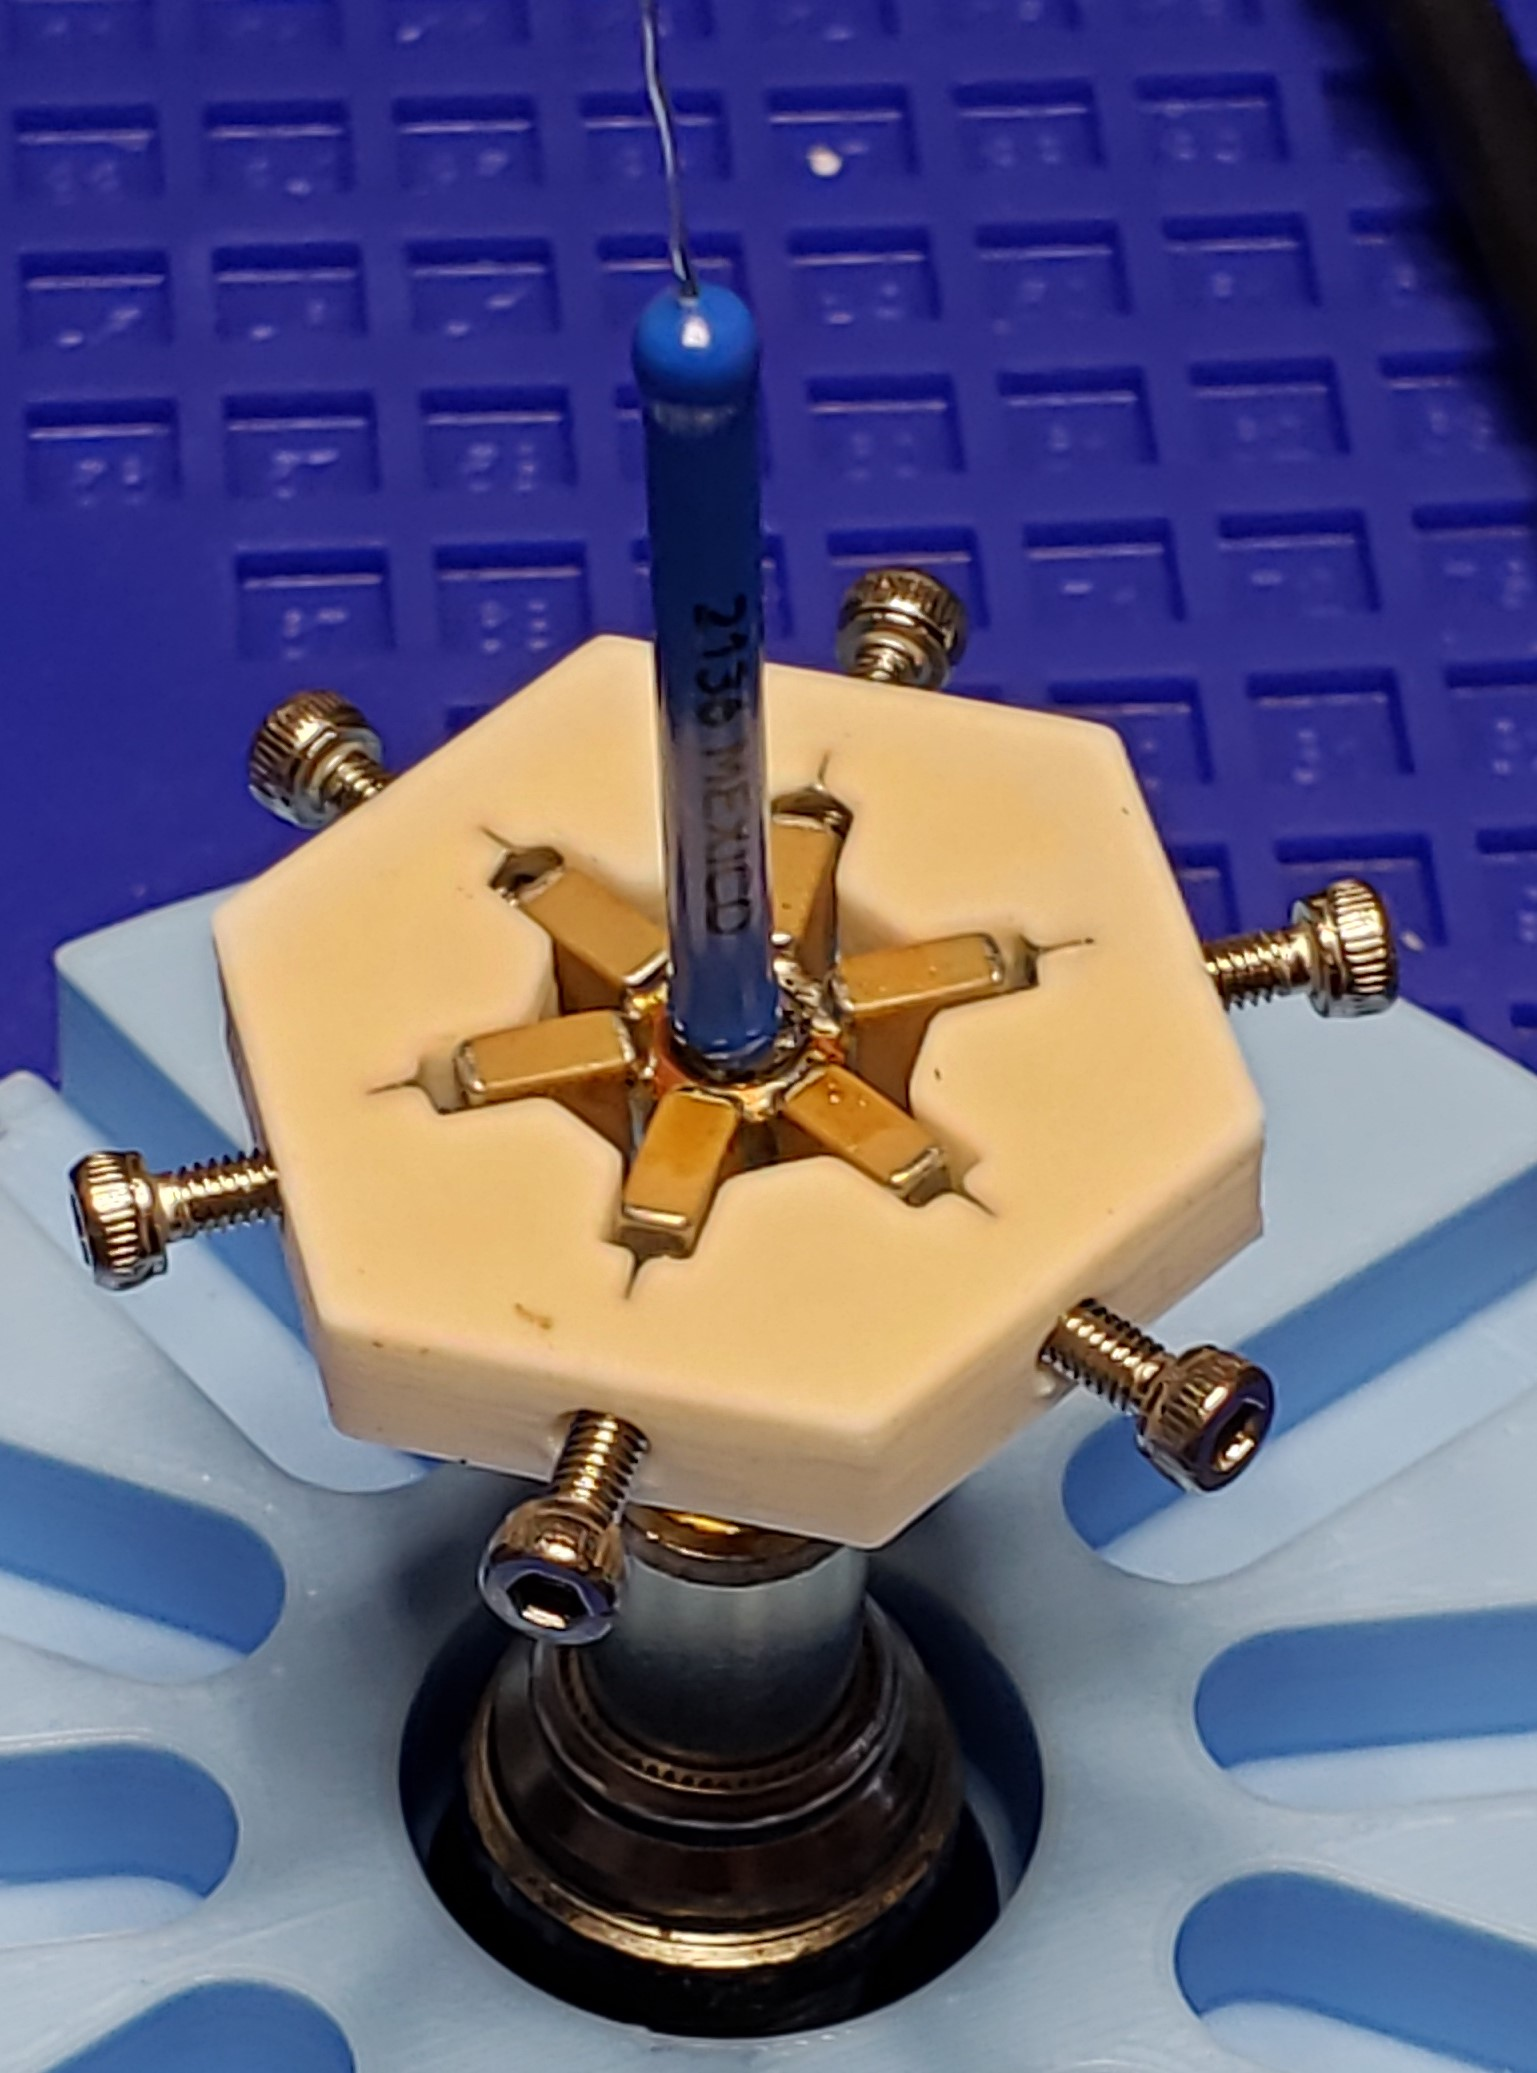
\includegraphics[height=3in]{FilterInternalSolderSupport}

\caption{Left: capacitors test fit in tube. Right: SHV jack, inpout resistor,
capacitors, and output resistor supported by SHV jack for soldering. }

\end{figure}
\end{enumerate}

\section{Attach the cable and tube}

\subsection{Attach the cable}

Assembly differs if the cable has a connector already that prevents
adding the tube after the cable is already attached. If the cable
doesn't have a connector on the end then not adding the tube until
after the cable is attached makes it easier to handle.
\begin{enumerate}
\item Cut a few millimeters of AWG 20 furrule and trim the resistor lead
and cable center conductor to fit inside the furrule.
\item Tin the resistor lead and cable center conductor, leave a large solder
blub so it will fill the furrle.
\item The furrle has a copper body but is nickel plated, which is hard to
remove from inside the tube and makes it hard to solder to. However,
the solder joint between the resistor and wire should be good.
\item Slide the furrule over the resistor lead while heating the furrule
until the solder melt and the furrle slides on fully.
\begin{enumerate}
\item If the cable has a connector already, slide the cable through the
grommet and tube first.
\end{enumerate}
\item Heat the furrule and slide the cable all the way into the furrule.
\item Gently tug on the cable to ensure it made a good connection.
\item Ensure there are no solder points that might cause discharges. No
solder is required on the exterior of the tube, whcih should minimize
the liklihood of pints. If the solder is hot enough before the heat
is removed it will form a smooth surface before solidifying. If there
is excessive solder on the tube exterior forming points, wick it away.
\item Clean the solder flux off the filter, this is the last chance to do
so before the tube prevents easy access to the filter internals.
\end{enumerate}

\subsection{Install the tube}
\begin{enumerate}
\item Remove any protective tape inside the filter and slide the tube into
place. Ensure the capacitor pads are visable through the holes in
the sides of the tube.
\begin{figure}[H]
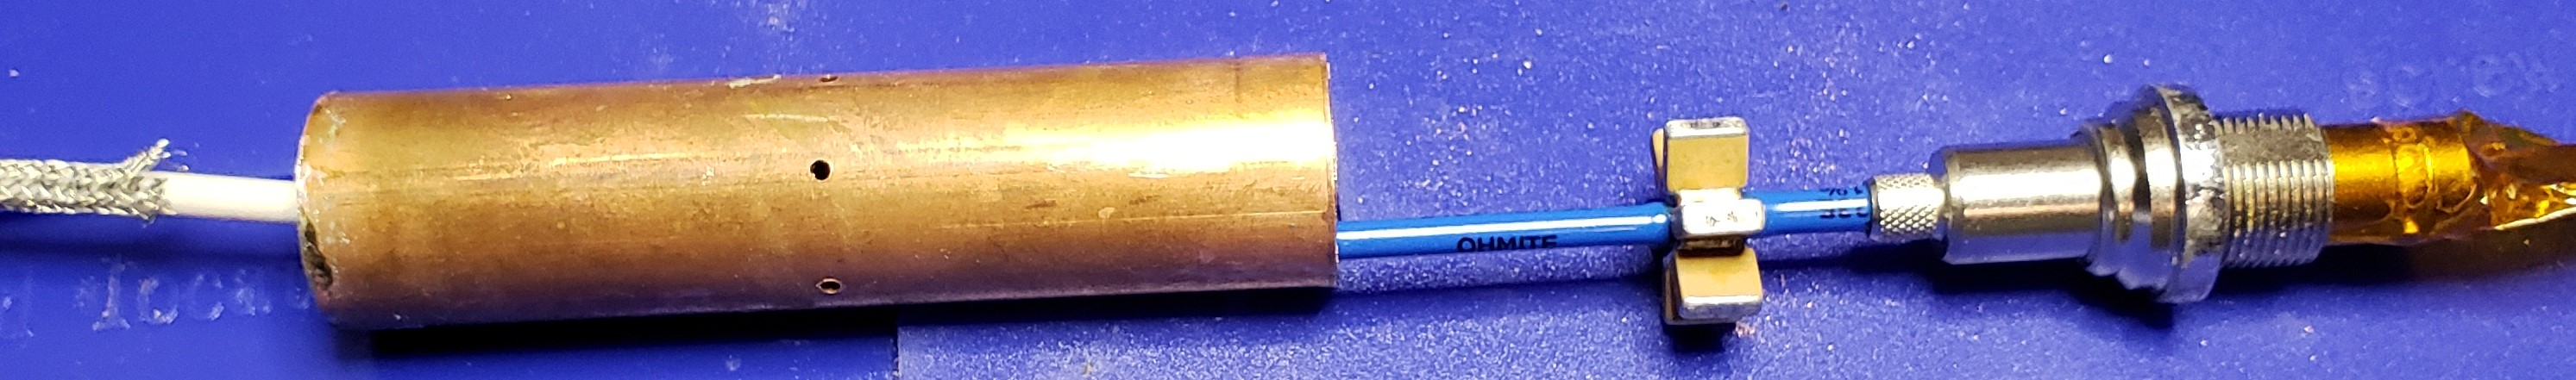
\includegraphics[width=5in]{FilterInternalInsertion}

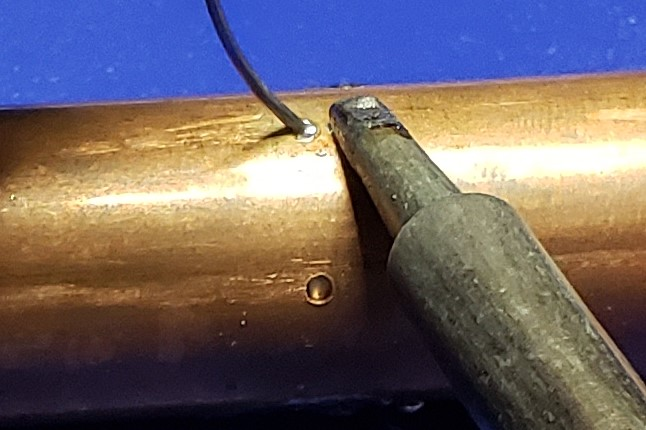
\includegraphics[height=2in]{FinalCapacitorSoldering}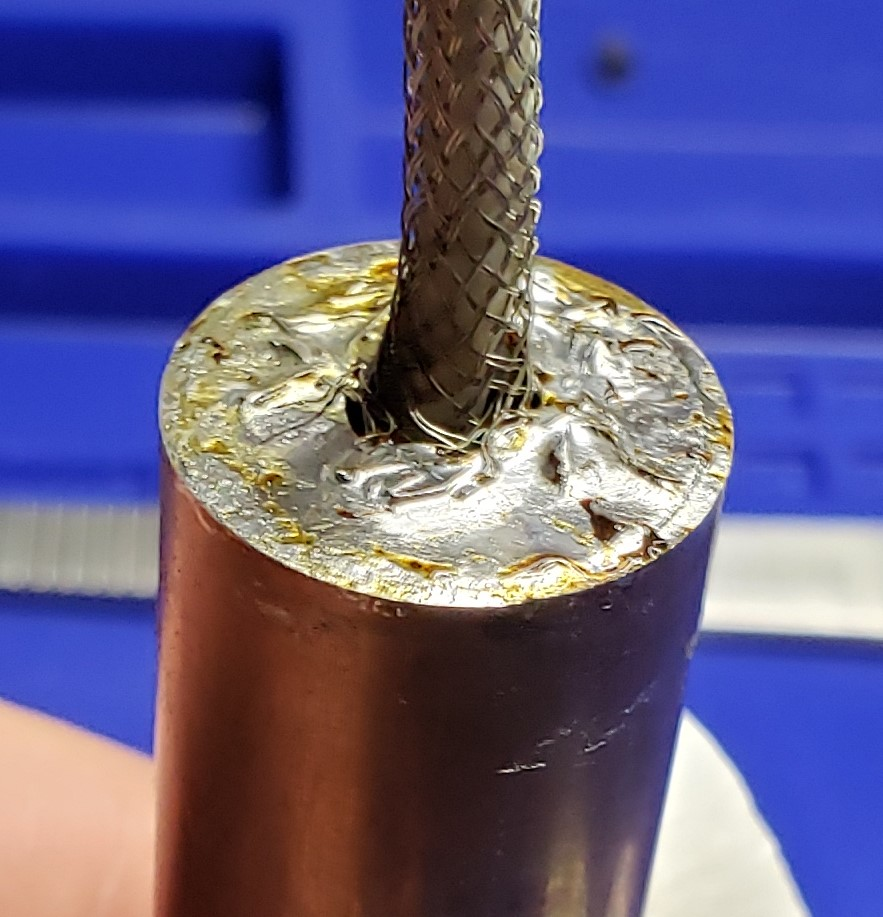
\includegraphics[height=2in]{FinalBraidSoldering}\caption{Filter assembly just before tube is slide into position.}
\end{figure}
\item Heat the tube right next to the holes and feed solder into the hole
until it flows in and joints the tube to the capacitor. Make sure
the holes are filled, these are oil boundries.
\item Solder the SHV jack to the tube. Ensure there are no gaps as this
is an oil seal.
\item Solder the end of the braid to the washer, make sure no stray wires
go into the hole that could cause discahrges. This gap will be filled
with epoxy.
\end{enumerate}
\textbf{\large{}4.3 Clean solder with a heavy-duty flux remover}{\large\par}

Materials needed: 413 B-Liquid, glass beaker, syringe with needle
tip, gloves, lab and glasses. 

To ensure that all the flux is removed and does not contribute to
the discharges, it is recommended to clean the solder components,
especially the pulser board, with heavy duty flux removal. The compound
used is 413 B-Liquid. The liquid contains acetone, which is highly
flammable. Gloves and glasses must be worn at all time while handling
the liquid, and cure must be maintained to not breathe in the liquid
fumes. Use only small amount of liquid at times. Acetone can disolve
plastic. Thus it is important to not let the liquid touch the 3D printed
endcaps and end ground break insulator to the SHV pin. 
\begin{enumerate}
\item Pour a small amount of 413 B-Liquid into the beaker. 
\item Draw the liquid into the syringe 
\item While holding the file with the pulse board on the bottom, put some
liquid into the filter using the small port holes 
\item Swirl for a few seconds. 
\item Repeat one more time to ensure all flux is removed. 
\item Carefully pour the solution back into a beaker. 
\item Use a KimTech wipe to wipe down liquid around the filter 
\item Use an empty syringe to purge the filter several times with air. This
will help dry out remaining liquid. 
\item Let the filter dry for atleast an hour. 
\item Let remaining liquid in the cup evaporate in a well ventilated area,
idially the fume hood in room 163.
\end{enumerate}

\section{Sealing the cable connection}
\begin{enumerate}
\item Hold the filter connector end up and flow isopropyl alcohol in through
the fill hole, letting it drain out the gap between the washer and
cable.
\begin{enumerate}
\item This is the last chance to clean the filter by flushing fluid through
the filter. Unless an optional drain hole is added to the output end
of the filter it can only be cleaned by filling and draining through
the same hole, which won't be as effective, once the cable connection
is sealed.
\end{enumerate}
\item Mix some epoxy and apply it generously to the gap between the washer
and cable. It isn't critical to keep the expoy from flowing into the
filter but the point is to seal the gap, not pot the filter.
\item Slide the cable grommet into position to hold the epoxy in while it
cures. Any voids in the epoxy on the filter exterior side of the washer
will not be exposed to high electric field and are of no concern for
discharges.
\item Tape around to grommet to ensure the epoxy remains in place while
it cures. 
\item Hold the filter connector end up so the epoxy flows into the gap and
seals as it cures.
\begin{figure}[H]
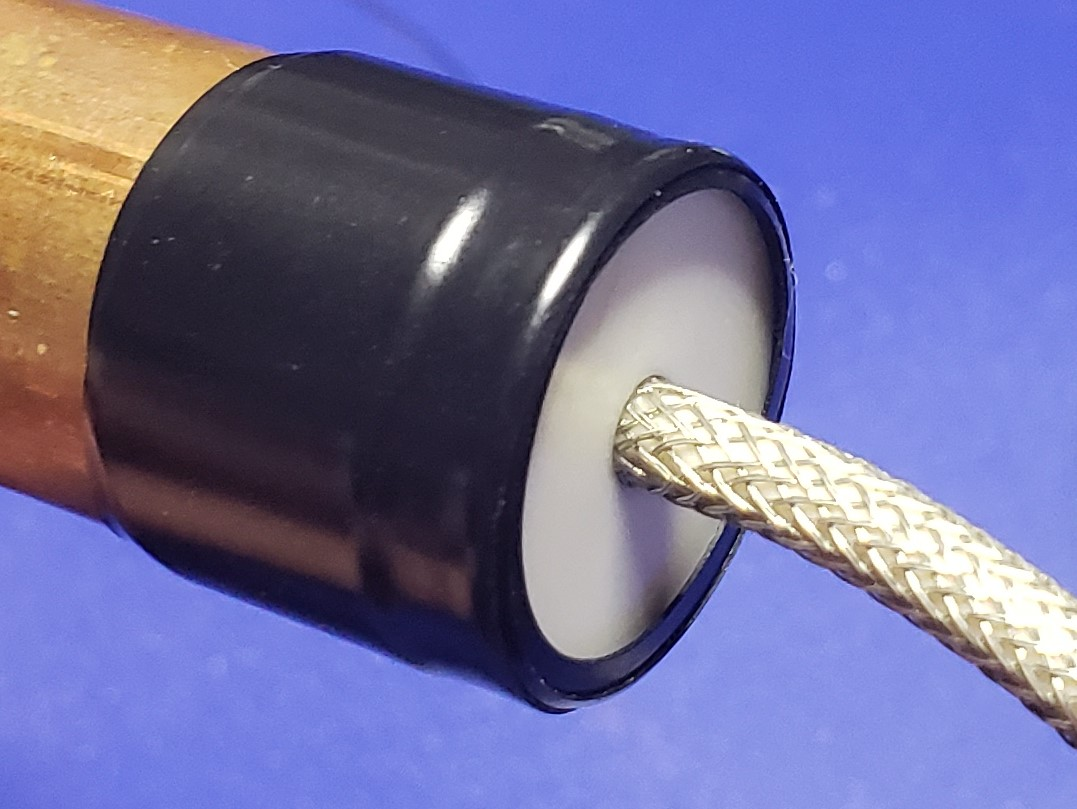
\includegraphics[angle=-90,width=3in]{FinalGrommetEpoxy}\caption{Grommet taped to end of filter to hold epoxy in place while it cures.}

\end{figure}
\end{enumerate}

\section{Fill the filter with oil}
\begin{enumerate}
\item Turn the filter on its side so the fill hole is up.
\item Use a syringe with a blunt needle to dispense oil into the fill hole.
\item Tilt the filter to ensure oil flows into crevices in the connector
end as well as the cable end. It should be as full as reasonably achievable.
\item Cover the hole in tape. Pull the tape tight and wrap it all the way
around the filter to ensure it doesn't come loose.
\item Keep it connector side down for a day to ensure there are no voids
in the oil near the high voltage pin of the connector. After this
any small voids in the oil will flow to regions of the filter that
are adjacent to the tube of the connector and not be a problem.
\begin{figure}

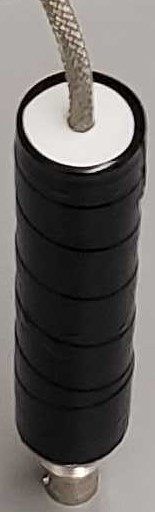
\includegraphics[width=2in]{FinishedFilter}\caption{Finished filter with electrical tape wrapped around entire length.}

\end{figure}
\end{enumerate}

\end{document}
